%%%%%%%%%%%%%%%%%%%%%%% file template.tex %%%%%%%%%%%%%%%%%%%%%%%%%
%
% This is a general template file for the LaTeX package SVJour3
% for Springer journals.          Springer Heidelberg 2010/09/16
%
% Copy it to a new file with a new name and use it as the basis
% for your article. Delete % signs as needed.
%
% This template includes a few options for different layouts and
% content for various journals. Please consult a previous issue of
% your journal as needed.
%
%%%%%%%%%%%%%%%%%%%%%%%%%%%%%%%%%%%%%%%%%%%%%%%%%%%%%%%%%%%%%%%%%%%
%
% First comes an example EPS file -- just ignore it and
% proceed on the \documentclass line
% your LaTeX will extract the file if required
\begin{filecontents*}{example.eps}
%!PS-Adobe-3.0 EPSF-3.0
%%BoundingBox: 19 19 221 221
%%CreationDate: Mon Sep 29 1997
%%Creator: programmed by hand (JK)
%%EndComments
gsave
newpath
  20 20 moveto
  20 220 lineto
  220 220 lineto
  220 20 lineto
closepath
2 setlinewidth
gsave
  .4 setgray fill
grestore
stroke
grestore
\end{filecontents*}
%
\RequirePackage{fix-cm}
%
%\documentclass{svjour3}                     % onecolumn (standard format)
%\documentclass[smallcondensed]{svjour3}     % onecolumn (ditto)
%\documentclass[smallextended]{svjour3}       % onecolumn (second format)
\documentclass[twocolumn]{svjour3}          % twocolumn
%
\smartqed  % flush right qed marks, e.g. at end of proof
%
\usepackage{graphicx}
\usepackage{times}
\usepackage{epsfig}
\usepackage{epstopdf}
\usepackage{amsmath}
\usepackage{amssymb}
\usepackage{subfigure}
\usepackage{caption}
\usepackage{tabularx}
\usepackage[table]{xcolor}
% Strike through text
 \usepackage[normalem]{ulem}
\usepackage{algorithm}
\usepackage[noend]{algpseudocode}
%
% \usepackage{mathptmx}      % use Times fonts if available on your TeX system
%
% insert here the call for the packages your document requires
%\usepackage{latexsym}
% etc.
%
% Somethong for pseudo algorithms
\makeatletter
\def\BState{\State\hskip-\ALG@thistlm}
\makeatother
% COLORS
\definecolor{myGreen}{HTML}{33FF00}
\definecolor{myRed}{HTML}{FF3030}
\definecolor{myGrey}{HTML}{AA5555}
\definecolor{myWhite}{HTML}{FFFFFF}
\definecolor{maroon}{cmyk}{0,0.87,0.68,0.32}
\definecolor{petr}{HTML}{5555FF}
% please place your own definitions here and don't use \def but
% \newcommand{}{}
\newcommand{\PP}{\mathbb{P}}
\newcommand{\Ncal}{N_{\text{c}}}
\newcommand{\subw}{0.20\linewidth}
\newcommand{\wii}{0.323\linewidth}
\newcommand{\diag}{\mathop{\mathrm{diag}}}

\renewcommand{\algorithmicrequire}{\textbf{Input:}}
\renewcommand{\algorithmicensure}{\textbf{Output:}}

%
% Insert the name of "your journal" with
\journalname{IJCV}
%
\begin{document}

\title{Learning and calibrating per-location classifiers for visual place recognition\thanks{Grants or other notes
about the article that should go on the front page should be
placed here. General acknowledgments should be placed at the end of the article.}
}
%\subtitle{...and learning compact descriptors}

%\titlerunning{Short form of title}        % if too long for running head

\author{Petr Gron{\'a}t         \and
        Josef {S}ivic          \and
        Tom{\'a}{\v s} Pajdla   \and
        Guillaume Obozinski%etc.
}

%\authorrunning{Short form of author list} % if too long for running head

\institute{F. Author \at
              first address \\
              Tel.: +123-45-678910\\
              Fax: +123-45-678910\\
              \email{fauthor@example.com}           %  \\
%             \emph{Present address:} of F. Author  %  if needed
           \and
           S. Author \at
              second address
}
\vspace{-5mm}
\date{Received: date / Accepted: date}
% The correct dates will be entered by the editor
%\maketitle
%***********************************************************
% *** THIS puts a figure between title and abstract ***
\twocolumn
[{%
    \renewcommand\twocolumn[1][]{#1}%
    \maketitle
    \begin{center}
        \centering
        \vspace*{-2mm}
        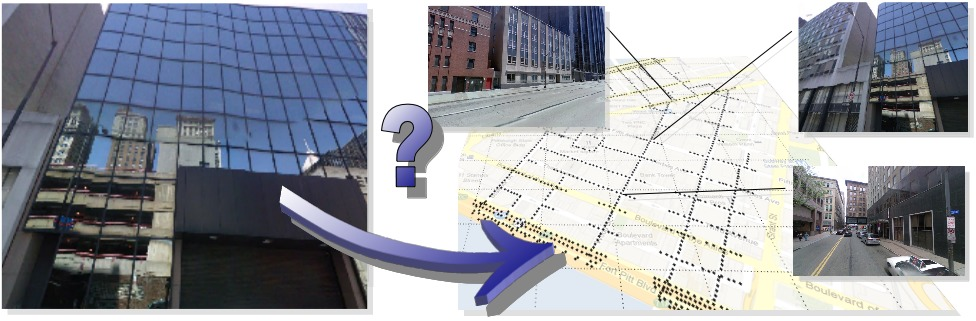
\includegraphics[width=.85\textwidth]{imgs/titleTeX.jpg}
        \vspace*{-2mm}
        \captionof{figure}
        {
          The goal of this work is to localize a query photograph (left) by finding other images of the same place in a large geotagged image database (right). 
          We cast the problem as a classification task and learn a classifier for each location in the database. 
          We develop two procedures
          to calibrate the outputs of the large number of per-location classifiers without the need for additional labelled training data.                     
%          We develop a non-parametric \textcolor{myGrey}{(can we asy tis for FV w-norm norm?)} procedure to calibrate the outputs of the large number of per-location classifiers without the need for additional positive training data.  
        }
    \end{center}%
}]
% ******************************************************

%\maketitle

\begin{abstract}
The aim of this work is to localize a query photograph by finding other images depicting the same place in a large geotagged image database. 
This is a challenging task due to changes in viewpoint, imaging conditions and the large size of the image database. The contribution of this work is two-fold. First, we cast the place recognition problem as a classification task and use the available geotags to train a classifier for each location in the database in a similar manner to per-exemplar SVMs in object recognition. 
Second, as only few positive training examples are available for each location, we propose 
two methods to calibrate all the per-location SVM classifiers without the need for additional positive training data.
The first method relies on p-values from statistical hypothesis testing and uses only the available negative training data. The second method performs an affine calibration by appropriately normalizing the learnt classifier hyperplane and does not need any additional labelled training data.
We test the proposed place recognition method with the bag-of-visual-words and Fisher vector image representations suitable for large scale indexing. 
Experiments are performed on two databases of 25,000 and 55,000 geotagged street view images of Pittsburgh and demonstrate improved place recognition accuracy of the proposed approach over the previous work.
% Add SF: as well as the San Francisco dataset containing 1M geotagged images
%\textcolor{myGrey}{
%Second, as only few positive training examples are available for each location, we propose a new approach to calibrate all the per-location SVM classifiers using \emph{only} the negative examples. The calibration we propose relies on a significance measure essentially equivalent to the p-values classically used in statistical hypothesis testing. Experiments are performed on a database of 25,000 geotagged street view images of Pittsburgh and demonstrate improved place recognition accuracy of the proposed approach over the previous work.
%\emph{(FV calibration)}}
\keywords{Place recognition \and classifier calibration \and Visual geo-localization}
% \PACS{PACS code1 \and PACS code2 \and more}
% \subclass{MSC code1 \and MSC code2 \and more}
\end{abstract}
%%%%%%%%%%%%%%%%%%%%%%%%
\section{Introduction}
%%%%%%%%%%%%%%%%%%%%%%%%
   \label{intro}
   Visual place recognition~\cite{Cummins09,Knopp2010,Schindler07} is a challenging task as the query and database images may depict the same 3D structure (e.g.\ a building) from a different camera viewpoint, under different illumination, or the building can be partially occluded. 
   In addition, the geotagged database may be very large. For example, we estimate that Google street-view of France alone contains more than 60 million panoramic images.
It is, however, an important problem as automatic, accurate and fast visual place recognition would have many practical applications in robotics, augmented reality or navigation.

  Similar to other work in large scale place recognition~\cite{Cummins09,Knopp2010,Schindler07,Torii2013} and image retrieval~\cite{Nister06,Philbin07,Sivic03,Jegou12} we describe each image by a set of local invariant features~\cite{Bay06,Lowe04} that are encoded and aggregated into a fixed-length single vector descriptor for each image. In particular, in this work we consider the sparse tf-idf weighted bag-of-visual-words representation~\cite{Sivic03,Philbin07} and the compact Fisher vector descriptors~\cite{Jegou12}.  
  
  The resulting vectors are then normalized to have unit $L_2$ norm and the similarity between the query and a database vector is measured by their dot product. This representation has some desirable properties such as robustness to background clutter and partial occlusion. Efficient retrieval can then achieved using inverted file indexing.


   While in image retrieval  databases are typically unstructured collections of images, place recognition databases are usually structured: images have geotags, are localized on a map and depict a consistent 3D world. %~\cite{Gronat2011}. 
   Knowing the structure of the database can lead to significant improvements in both speed and accuracy of place recognition. 
   Examples include: (i) building an explicit 3D reconstruction of the scene~\cite{Irschara2009,Li10,Li12}; (ii) constructing an image graph~\cite{Cao13,Philbin10c,Turcot09}, where images are nodes and edges connect close-by images on the map~\cite{Torii11}, or (iii) using the geotagged data as a form of supervision to select local features that characterize a certain location~\cite{Knopp2010,Schindler07} or re-rank retrieved images~\cite{Zamir10}.

  In this work, we also take advantage of geotags as an available form of supervision and investigate whether the place recognition problem can be cast as a classification task.
  Visual classifiers were investigated for landmark~\cite{Li09} recognition in consumer photo collections, where many photographs are available for each landmark.
  In this work we wish to recognize individual locations from street-level imagery where only a few (1-5) photographs are available for each place. 
  Therefore, we train a classifier {\em for each location on the map} in a similar manner to per-exemplar classification in object recognition~\cite{Malisiewicz11}. 

  This is beneficial as  each classifier can learn which features are discriminative for a particular place. % and down-weight features occurring at other places.
   The classifiers are learnt offline. At query time, the query photograph is localized by transferring the GPS tag of the best scoring location classifier.

  While learning classifiers for each place may be appealing, calibrating outputs of the individual classifiers is a critical issue. In object recognition~\cite{Malisiewicz11}, it is addressed in a separate calibration stage on a held-out set of training data.
  This is not possible in the place recognition set-up as only a small number, typically one to five, of positive training images are available for each location (e.g. street-view images viewing the same building facade). To address this issue, we propose two calibration methods. 
  The first method relies on p-values from statistical hypothesis testing and uses only the available negative training data. The second method performs a simple affine calibration by appropriately normalizing the learnt classifiers and does not need any additional labelled calibration examples.   


%%%%%%%%%%%%%%%%%%%%%%%%%%%%%%%%%
\section{Related work} 
\label{sec:related}
%%%%%%%%%%%%%%%%%%%%%%%%%%%%%%%%%

\paragraph{Large-scale visual place recognition.}
    The visual localization problem is typically treated as large-scale instance-level retrieval~\cite{Cummins09,Chen11,Gronat13,Knopp2010,Schindler07,Torii2013,Zamir10}, where images are represented using local invariant
    features~\cite{Lowe04} encoded and aggregated into the bag-of-visual-words~\cite{Csurka04,Sivic03} or Fisher vector~\cite{Jegou12} representations. 
    The image database can be further augmented by 3D point clouds~\cite{Klinger13}, automatically
    reconstructed by large-scale structure from motion
    (SfM)~\cite{Agarwal-ICCV-2009,Klinger13}, which enables accurate prediction of query image camera position~\cite{Li12,Sattler12}.
    In contrast, in this work we investigate learning a discriminative place-specific image representation. A similar idea has been recently explored in~\cite{Cao13} 
    who learn a graph-based discriminative representation for landmark image collections where typically many images are available for each place.
    In this work, we focus on street-level images such as Google street-view, which have greater coverage, but typically only one or a small number of images are  available for each place.  To address this issue we learn a discriminative re-weighting of the descriptor specific to each image in the database using per-exemplar support vector machine~\cite{Malisiewicz11}.
    
    
\paragraph{Per-exemplar support vector machine.} 
    The exemplar support vector machine (e-SVM) has been used in a number of visual recognition tasks including
    category-level recognition~\cite{Malisiewicz11}, cross-domain retrieval~\cite{Shrivastava11}, scene parsing~\cite{Tighe13}, %image to 3D model alignment~\cite{Aubry13},
    place recognition~\cite{Gronat13} or as an initialization  for more complex discriminative clustering models~\cite{Doersch12,Singh12}. The main idea is to train a linear support vector machine (SVM) classifier from a single positive example and a large number of negatives. The intuition is that the resulting weight vector will give a higher weight to the discriminative dimensions of the positive training data point and will down weight dimensions that are non-discriminative with respect to the negative training data. A key advantage is that each per-exemplar classifier can be trained independently and hence the learning can be heavily parallelized. 
    The per-exemplar training brings however also an important drawback. As each classifier is trained independently a
    careful calibration of the resulting classifier scores is required~\cite{Malisiewicz11}. 

\paragraph{Calibrating classifier scores.} 
  Several calibration approaches have been proposed in the literature (see~\cite{gebel2007calibrating} and references therein for a review). The most known consists of fitting a logistic regression to the output of the SVM~\cite{Platt99}.  This approach, however, has a major drawback as it imposes a parametric form (the logistic a.k.a.\ sigmoid function) of the likelihood ratio of the two classes, which typically leads to biased estimates of the calibrated scores. Another important calibration method is the isotonic regression~\cite{zadrozny2002transforming}, which allows for a non-parametric estimate of the output probability.
  Unfortunately, the fact that we have only a single positive example (or only very few of them, and which are all used for training) essentially prevents us from using any of these methods. 
  To address these issues, we develop two classifier calibration methods that do not need additional labelled positive examples. Related to ours is also the recent work of Scheirer et al.~\cite{Scheirer12} who develop a classifier calibration method for face attribute similarity search. Their method (discussed in more detail in section~\ref{sec:calibration}) also does not require labelled positive examples but, in contrast to us, uses a parametric model (the Weibull distribution) for the scores of negative examples.    


\paragraph{Contributions.} 
  This paper has two main contributions. First, we cast the place recognition problem as a classification task and use the available geo-tags to train a classifier for each location in the database (section~\ref{sec:classifiers}). Second, as only few positive training examples are available for each location, we propose two methods to calibrate all the per-location SVM classifiers without the need for additional positive training data. The first method (section~\ref{sec:calibration}) relies on p-values from statistical hypothesis testing. The second method (section~\ref{sec:calibrationRenorm}) performs an affine calibration by appropriately normalizing the learnt decision hyperplane. 
  We also describe a memory efficient classifier representation for the sparse bag-of-visual-word vectors (section~\ref{sec:memory}) and  experimentally demonstrate benefits of the proposed approach (section~\ref{sec:experiments} and~\ref{sec:results}). 


%%%%%%%%%%%%%%%%%%%%%%%%
\section{Per-location classifiers for place recognition}
\label{sec:classifiers}
%%%%%%%%%%%%%%%%%%%%%%%%
   We are given an image descriptor $\vec{x}_j$, one for each database image $j$. This representation can be a sparse tf-idf weighted bag-of-visual-words vector~\cite{Sivic03} or a dense compact descriptor such as the Fisher vector (FV)~\cite{Jegou12}. The goal is to learn a score $f_j$ for each database image $j$, so that, at test time, given the descriptor $\vec{q}$ of the query image, we can either retrieve the correct target image as the image $j^*$ with the highest score
   % 
   \begin{equation}
   \label{eq:class}
    j^*=\operatorname*{arg\;max}_{j} f_j(\vec{q}) 
   \end{equation}
    %
   \noindent
   or use these scores to rank candidate images and use geometric verification to identify the correct location in an $n$-best list.
   Instead of approaching the problem directly as a large multiclass classification problem, we tackle the problem by learning a per-exemplar linear SVM classifier~\cite{Malisiewicz11}  for each database image $j$.
   Similar to~\cite{Knopp2010}, we use the available geotags to construct the negative set $\mathcal N_j$ for each image $j$. The negative set is constructed so as to concentrate difficult negative examples, i.e.\ from images that are far away from the location of image $j$ and at the same time similar to the target image as measured by the dot product between their feature vectors. The details of the construction procedure will be given in section~\ref{sec:experiments}.  The positive set $\mathcal P_j$ is represented by the only positive example, which is $\vec{x}_j$ itself. 
   Each SVM classifier produces a score $s_j$ which is a priori not comparable with the score of the other classifiers. A calibration of these scores will therefore be key to convert them to comparable scores $f_j$. This calibration problem is more difficult than usual given that we only have a single positive example and will be addressed in section~\ref{sec:calibration}.
   
   %%%%%%%%%%%%%%%%%%%%%%%%%%%%%%%%%%%%%%%%%%%%%%%%%%%
   \subsection{Learning per-location SVM classifiers }
   %%%%%%%%%%%%%%%%%%%%%%%%%%%%%%%%%%%%%%%%%%%%%%%%%%%
      Each linear SVM classifier learns a score $s_j$ of the form 
      %
      \begin{align}
        s_j(\vec{q})=\vec{q}^T \vec{w}_j+b_j
        \label{eq:linear}
      \end{align}
      %
      \noindent
      where $\vec{w}_j$ is a weight vector re-weighting contributions of individual visual words and $b_j$ is the bias specific for image $j$. Given the training sets $\mathcal P_j$ and $\mathcal N_j$, the aim is to find a vector $\vec{w}_j$ and bias $b_j$ such that the score difference between $\vec{x_j}$ and the closest neighbor from its negative set $\mathcal N_j$ is {\em maximized}. % modulo margin (perhaps mention this).
      Learning the weight vector $\vec{w}_j$ and bias $b_j$ is formulated as a minimization of the convex objective 
      %
      \begin{align}
        \nonumber
        \Omega(\vec{w}_j,b_j)=||\vec{w}_j||^{2}& +C_1\sum_{\vec{x}\in \mathcal P_j}h(\vec{w}_j^T\vec{x}+b_j)   \\
        \label{eq:obj}
                           & +C_2\sum_{\vec{x}\in \mathcal N_j}h(-\vec{w}_j^T\vec{x}-b_j), 
      \end{align}
      %
      \noindent
      where the first term is the regularizer, the second term is the loss on the positive training data weighted by scalar parameter $C_1$, and the third term is the loss on the negative training data weighted by scalar parameter $C_2$.   
      This is a standard SVM formulation \eqref{eq:obj}, also used in exemplar-SVM~\cite{Malisiewicz11}.
      In our case $h$ is the squared hinge loss, which we found to work better in our setting than the standard hinge-loss. $\vec{w}_j$ and $b_j$ are learned separately for each database image $j$ in turn. 
     
  %%%%%%%%%%%%%%%%%%%%%%%%%%%%%%%%%%%%%%%%%%%%%%%%%%%
  \subsection{The need for calibrating classifier scores}
  %%%%%%%%%%%%%%%%%%%%%%%%%%%%%%%%%%%%%%%%%%%%%%%%%%%
    Since the classification scores $s_j$ are learned independently for each location $j$, they cannot be directly used for place recognition as in eq.~\eqref{eq:class}. As illustrated in figure~\ref{fig:calib}, for a given query $\vec{q}$, a classifier from an incorrect location (b) can have a higher score~\eqref{eq:linear} than the classifier from the target location (a). Indeed, the SVM score is a signed distance from the discriminating hyperplane and is a priori not comparable between different classifiers. This issue is addressed by calibrating scores of the learnt classifiers. The goal of the calibration is to convert the output of each classifier into a probability (or in general a ``universal" score), which can be meaningfully compared across classifiers. In the following two sections we develop two classifier calibration methods that do not need additional labelled positive examples.
 
%%%%%%%%%%%%%%%%%%%%%%%%%%  
\section{Non-parametric calibration of the  SVM-scores from negative examples only}
\label{sec:calibration}
%%%%%%%%%%%%%%%%%%%%%%%%%%  

In this section we describe a classifier calibration method that exploits the availability of large amounts of negative data, i.e.\ images from other far away locations in the database.
In particular, the method estimates the significance of the score of a test example compared to the typical score of  the (plentifully available) negative examples. Intuitively, we will use a large dataset of negative examples to calibrate the individual classifiers so that they {\em reject the same number of negative examples} at each level of the calibrated score.   We will expand this idea in detail using the concepts from hypothesis testing. % to propose a calibration method.


   %%%%%%%%%%%%%%%%%%%%%%%%%%%%%%%%%%%%%%%%%%%%%%%%%%%%%%%
   \subsection{Calibration \emph{via} significance levels}
   %%%%%%%%%%%%%%%%%%%%%%%%%%%%%%%%%%%%%%%%%%%%%%%%%%%%%%% 
      In the following, we view  the problem of deciding whether a query image matches a given location based on the corresponding SVM score as a hypothesis testing problem. In particular, we appeal to ideas from the traditional frequentist hypothesis testing framework also known as Neyman-Pearson (NP) framework (see e.g.~\cite{casella2001statistical}, chap.~8).

      We define the null hypothesis as $H_0=\{$the image is a random image$\}$ and the alternative as $H_1=\{$the image matches the particular location$\}$. The NP framework focuses on the case where the distribution of the data under $H_0$ is well known, whereas the distribution under $H_1$ is not accessible or too complicated to model, which matches perfectly our setting.

      In the NP framework, the \emph{significance level} of a score is measured by the p-value or equivalently by the value of the cumulative density function  (cdf) of the distribution of the negatives at a given score value. The cdf is the function $F_0$ defined by $F_0(s)=\PP(S_0\leq s)$, where $S_0$ is a random variable corresponding to the scores of negative data (see figure~\ref{fig:qntExample} for an illustration of the relation between the cdf and the density of the function). The cdf 
      (or the corresponding p-value\footnote{
        The notion most commonly used in statistics is in fact the p-value. The p-value associated to a score is the quantity $\alpha(s)$ defined by $\alpha(s)=1-F_0(s)$; so the more significant the score is, the closer to $1$ the cdf value is, and the closer to $0$ the p-value is. To keep the presentation simple, we avoid the formulation in terms of p-values and we only talk of the probabilistic calibrated values obtained from the cdf $F_0$.
       }
      )
      is naturally estimated by the empirical cumulative density function $\hat{F}_0$, which is computed as: 
      %
      \begin{equation}
        \hat{F}_0(s)=\frac{1}{\Ncal} \sum_{n=1}^{\Ncal} 1_{\{s_n \leq s\}},
        \label{eq:empiricalCDF}
      \end{equation}
      %
      \noindent
      where $(s_n)_{1\leq n \leq \Ncal }$ are the SVM scores associated with $\Ncal$ negative examples used for calibration. \textcolor{petr}{Notice that positive example is not involved in construction the cumulative density function.}
      $\hat{F}_0(s)$ 
      is the fraction of the negative examples used for calibration (ideally held out negative examples) that have a score below a given value $s$.
      Computing $\hat{F}_0$ exactly would require to store all the SVM scores for all the calibration data for all classifiers, so in practice, we only keep a fraction of the larger scores.
      We also interpolate the empirical cdf between consecutive datapoints so that instead of being a staircase function it is a continuous piecewise linear function such as illustrated in figure~\ref{fig:calib}. Given a query, we first compute its SVM score $s_q$ and then compute the calibrated probability $f(q)=\hat{F}_0(s_q)$.
      We obtain a similar calibrated probability $f_j(q)$ for each of the SVMs associated with each of the target locations, which can now be ranked.
      \textcolor{petr}{
      Another example of score calibration is shown in figure~\ref{fig:3qVSw}. Each plot contains respective calibration cdf for particular target image and circles denote calibrated SVM score for three different images. Notice that while figure~\ref{fig:calib} displays only few datapoints of the cdf plots in figure~\ref{fig:3qVSw} show complete cdf consisting of $25k$ datapoints. Notice also that cumulative density functions in figure~\ref{fig:3qVSwfig:3qVSw} are similar but not identical.
      }
      %
      \begin{figure}[t]
         \vspace{1mm}
         \subfigure[]{
            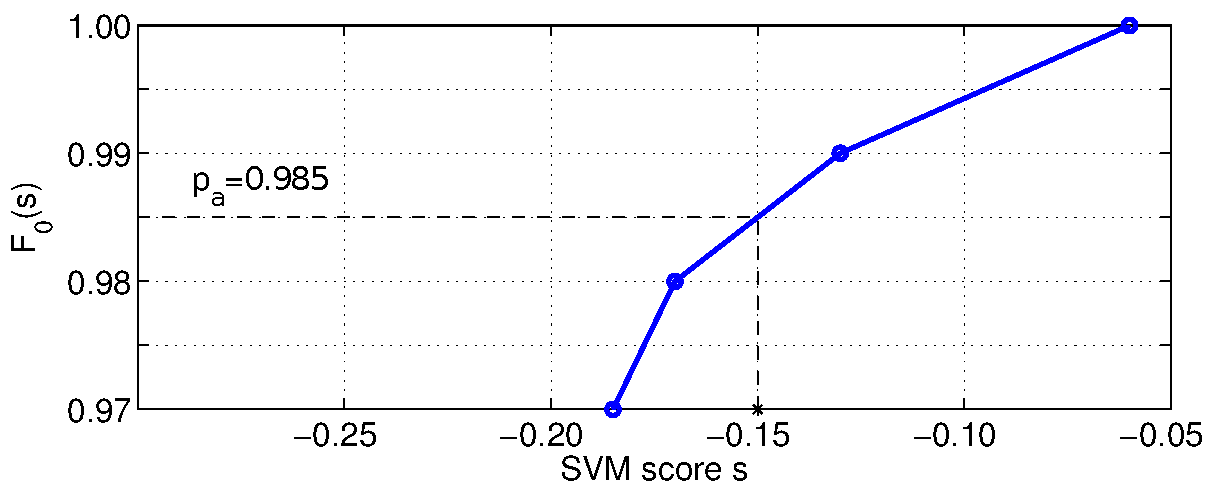
\includegraphics[width=\linewidth]{imgs/qnt1x}
            \label{fig:subfig1}
         }
         \vspace{1.5mm}\newline
         \subfigure[]{
            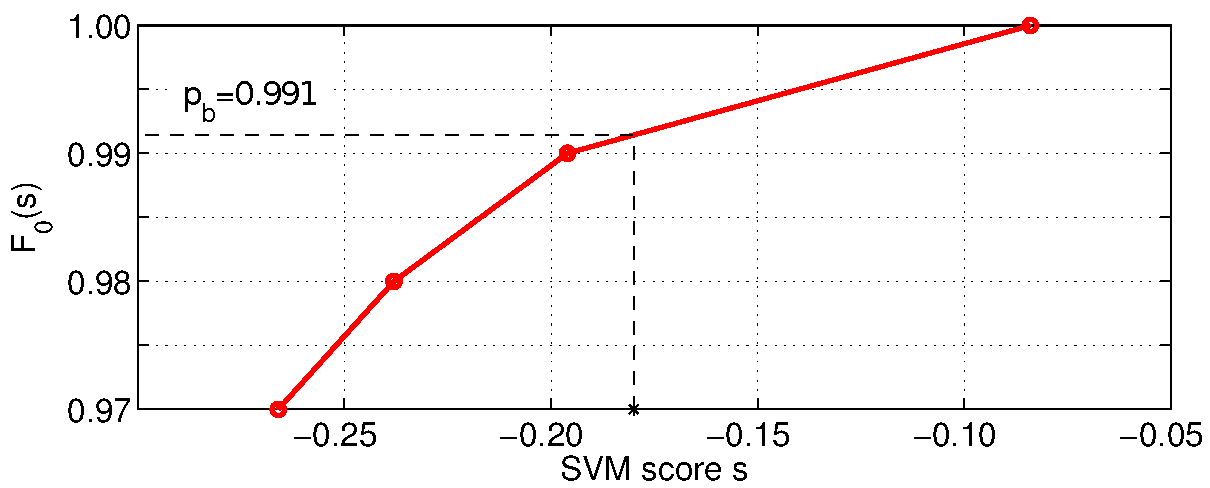
\includegraphics[width=\linewidth]{imgs/qnt2x}
            \label{fig:subfig2}
         }
         \vspace*{-3mm}
         \caption[]{
            \textbf{An illustration of the proposed normalization of SVM~scores for two different database images.}
            In each plot, the x-axis shows the raw SVM score. The y-axis shows the calibrated output. For the given query, the raw SVM score of image (b) is lower than for image (a), but the calibrated score of image (b) is higher than for image (a). 
         }
         \vspace*{-2mm}
         \label{fig:calib}
      \end{figure}

      \begin{figure}[t]
         \subfigure[]{
            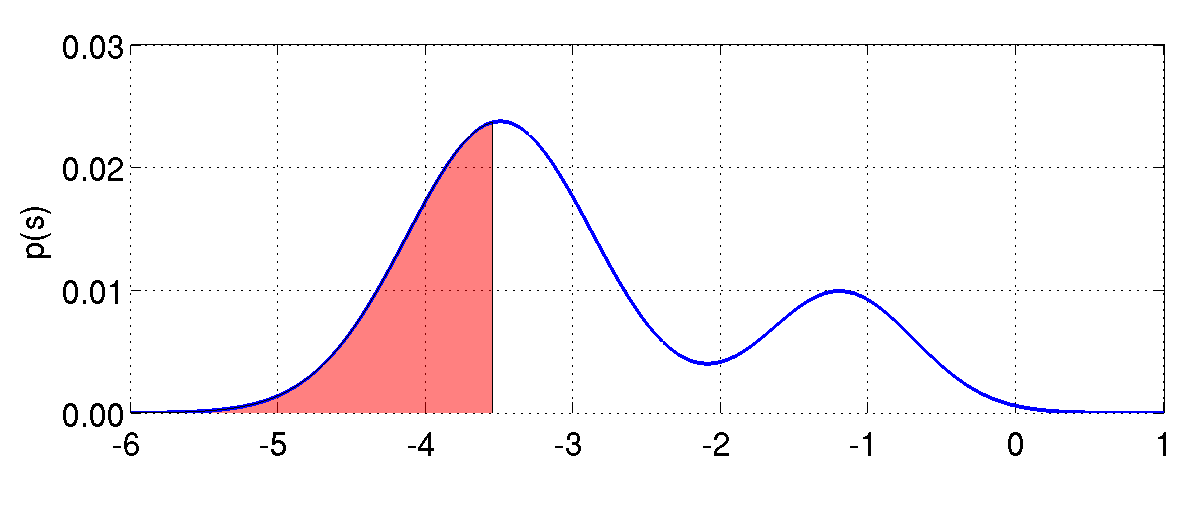
\includegraphics[width=\linewidth]{imgs/qntEx1.pdf}
         }
         \subfigure[]{
            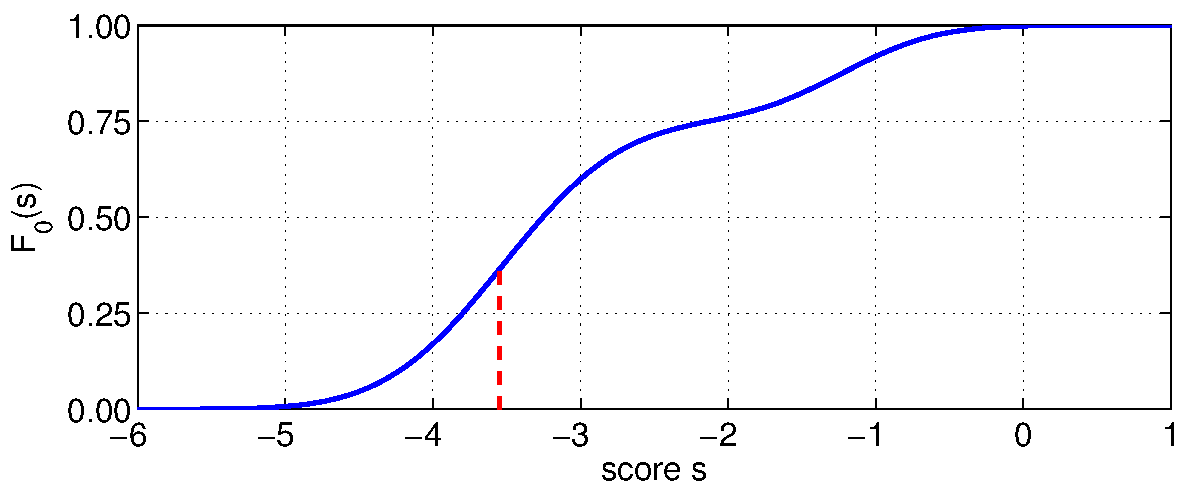
\includegraphics[width=\linewidth]{imgs/qntEx2.pdf}
         }
         \vspace*{-3mm}
         \caption{
         \textbf{Cumulative density function.}
         Illustration of the relation between (a) the probability density of the random variable $S_0$ modeling the scores of the negative examples and (b) the corresponding cumulative density function $F_0(s)=\PP(S_0 \leq s)$.
         }
               \vspace*{-3mm}
         \label{fig:qntExample}
      \end{figure}
      
      
   %%%%%%%%%%%%%%%%%%%%%%%%%%%%%%%%%%%%%%%%%%%%%%%%%
   \subsection{Summary of the calibration procedure}
   %%%%%%%%%%%%%%%%%%%%%%%%%%%%%%%%%%%%%%%%%%%%%%%%%
    
    For each trained place-specific classifier $s_j$ we construct the empirical cumulative density function~\eqref{eq:empiricalCDF} of scores of the negative examples and keep only its top $K$ values. This can be done offline and the procedure is summarized in Algorithm \ref{alg:offline}. 
    %
    At query time, given a query image descriptor $\vec{q}$, we compute the uncalibrated classification score $s_j(\vec{q})$ and then use the stored cdf values to compute the calibrate score $f_j(\vec{q})$. This procedure is performed for each database image $j$ and is summarized in Algorithm \ref{alg:online}.
    Finally, the best candidate database image is selected by equation~\eqref{eq:class}. Alternatively, candidate database images can be also ranked according to the calibrated score.
 
 
      \begin{algorithm}
          \caption{P-value calibration: offline stage}
          \label{alg:offline}
          \algorithmicrequire{\hspace{5mm}
            $\mathcal{X}$ \dots column wise matrix of image descriptors\newline  
            \textcolor{myWhite}{.\hspace{13mm}}$\vec{w}_j$, $b_j$ \dots learnt SVM weights and biases\newline
          }
          \algorithmicensure{\hspace{2mm} $\hat{F}_{0j}$ \dots calibration functions}
          \begin{algorithmic}[1]
              \Procedure{p-value calibration}{}
              \State $N \gets$ database size
              %\State $K \gets$ size of the cdf tail to be kept
              \State $\mathcal{X} \gets$ descriptor matrix of negative examples %all database images
              \For{$\forall j \in 1 \dots N$}
                \State $N_c \gets$ number of negative examples
                \State $\vec{w} \gets$ learned SVM weight for image $j$
                \State $b \gets$ learned SVM bias for image $j$
                \State $\vec{\sigma} \gets \vec{w}^T \mathcal{X}+b$
                \State {\em Compute the cdf:}  % $\vec{s_j}, \hat{F}_{0j}$ }
                \State $\vec{s_j} \gets$ sorted $\vec{\sigma}$ in descending order
                \State $\hat{F}_{0j} \gets [N_c \dots 0]/N_c$
              \EndFor
              \EndProcedure
         \end{algorithmic}
      \end{algorithm}

       \begin{algorithm}
          \caption{P-value calibration: online stage}
          \label{alg:online}
          \algorithmicrequire{\hspace{5mm}
              $\vec{q}$ \dots query image descriptor\newline  
              \textcolor{myWhite}{.\hspace{13mm}}$\vec{w}_j$, $b_j$ \dots learnt SVM weights and biases\newline
              \textcolor{myWhite}{.\hspace{13mm}}$\hat{F}_{0j}$ \dots learnt calibration function\newline
          }
          \algorithmicensure{\hspace{2mm} $f_j(\vec{q})$ \dots calibrated score}
          %
        \begin{algorithmic}[1]
              \Procedure{calibrating scores}{}
              \State $\vec{q} \gets$ query image descriptor
              \State $N \gets$ database size
              %         \State $y \gets [0,1,\dots (K-1)]$
              \For{$\forall j \in 1 \dots N$} // for each database image
                \State $\vec{w} \gets$ learned SVM weight for image $j$
                \State $b \gets$ learned SVM bias for image $j$
                \State $\hat{F}_{0} \gets \hat{F}_{0j}$ // Empirical cdf
                \State $\vec{s} \gets \vec{s_j}$ // Corresponding sorted scores
                \State $s_q \gets \vec{q}^T\vec{w}+b$  // compute uncalibrated classifier score 
              %		        \State $\hat{F}_0 \gets \hat{F}_{0j}$
                \State Find $n$ such that $s_{n} \leq s_q < s_{n+1} $
                \State Compute the interpolated empirical cdf value:
                \Statex $\hspace{9mm}
                  \hat{F}_0(s_q)\approx 
                  \hat{F}_0(s_n)+\frac{s_q-s_n}{s_{n+1}-s_n} (\hat{F}_0(s_{n+1})-\hat{F}_0(s_n)).
                $
                \State $f_j(\vec{q})=\hat{F}_0(s_q)$ // output the calibrated score

              \EndFor
              \EndProcedure
        \end{algorithmic}
      \end{algorithm}
      

   %%%%%%%%%%%%%%%%%%%%%%%
   \subsection{Discussion}
   \label{sec:discussion}
   %%%%%%%%%%%%%%%%%%%%%%% 
      It should be noted that basing the calibration only on the negative data has the advantage that we privilege precision over recall, which is justified given the imbalance of the available training data (much more negatives than positives).
      Indeed, since we are learning with a single positive example, intuitively, we cannot guarantee that the learned partition of the space will generalize well to other positives, whose scores in the test set can potentially drop significantly. % (this is indeed what we observe in practice). 
      By contrast, since we are learning from a comparatively large number of negative examples, we can trust the fact that new negative examples will stay in the half-space containing the negative training set, so that their scores are very unlikely to be large. Our method is therefore based on the fact that we can measure reliably how surprising a high score would be if it was the score of a negative example. This exactly means that we can control false positives (type I error) reasonably well but not false negatives (type II error or equivalently the power of our test/classifier), exactly as in the Neyman-Pearson framework.

      An additional reason for not relying on positive examples for the calibration in our case is that (even if we had sufficiently many of them) the positive examples that we collect using location and geometric verification from the geotagged database typically have illumination conditions that are extremely similar to each other and not representative of the distribution of test positives which can have very different illuminations. This is because of the controlled nature of the capturing process of geotagged street-level imagery (e.g.\ Google street-view) used for experiments in this work. Close-by images are typically captured at a similar time (e.g. on the same day) and under similar imaging conditions.

      Scheirer et al.~\cite{Scheirer12} propose a method, which is related to ours, and calibrate SVM scores by computing the corresponding cdf value of a Weibull distribution fitted to the top negative scores. The main difficulty is that the Weibull model should be fitted only to the tail of the distribution of the negatives, which is in general difficult to identify. As a heuristic, Scheirer et al. propose to fit the Weibul model to false positives (i.e. the negative samples classified incorrectly as positives). But in our case, most of the exemplar SVMs that we are training have zero false positives in a held out set, which precludes the application of their method. 
%      To avoid that issue our approach forgoes any parametric form of the distribution and instead relies directly on a standard non-parametric estimate of the cumulative density function.

      Finally, we should remark that we are not doing here calibration in the same sense of the word as the calibration based on logistic regression (or isotonic regression), since logistic regression estimates a probability of making a correct prediction by assigning a new data to class $1$, while we are estimating how unlikely it would be for a negative example to have such a high score. The calibration with either methods yields ``universal" scores in the sense that they are comparable from one SVM to another, but the calibrated values obtained from logistic regression are not comparable to the values obtained from our approach.

%%%%%%%%%%%%%%%%%%%%%%%%%%  
\section{Affine calibration by normalizing the classification hyperplane}
%\section{Calibration by-normalization }
\label{sec:calibrationRenorm}
%%%%%%%%%%%%%%%%%%%%%%%%%%  
  
  The non-parametric calibration method described in the previous section has two computational disadvantages, which make it hard to scale-up to very large datasets. 
  % of more than 1M images.  
  First, the method requires storing the non-parametric model of the calibration function for each learned classifier. This has memory complexity 
  of $O(NK)$, where $N$ is the number of images (classifiers) in the database and $K$ the number of stored elements of the non-parametric model. For typical values of $K=1000$ and $N=1$M this would require additional 4GB of memory, comparable to the size of the inverted index itself. Second, computing the cumulative density function requires applying all $N$ learnt classifiers to the entire set of negative examples, which has also size $N$. As a result computing the cdf has complexity $O(N^2)$, which becomes quickly infeasible already for datasets with $N$ larger than $100,000$. 
  
  To address these issues we first describe an affine calibration model that calibrates the classifier score with a simple linear function defined by only two parameters: its slope and offset, greatly reducing the required storage.
  %This greatly reduces the storage requirements and makes storing the calibration functions feasible for very large datasets.
  Second, we show that the parameters of the affine calibration function can be obtained by normalizing the learnt classification hyper-plane without applying the classifiers on the negative data and thus bringing down the computational complexity to $O(N)$.
  As a result,  computing and storing the calibration functions becomes feasible for very large datasets with 1M images.

  \subsection{Affine calibration model}
   Using the affine calibration model we transform the uncalibrated score $s_j(\vec{q})$ of query $\vec{q}$ with a linear function 
    %
     \begin{equation}
       f_j(\vec{q}) = \alpha_j s_j(\vec{q}) + \beta_j,
       \label{eq:affine}
     \end{equation}
     %
	where 
	$ f_j(\vec{q})$ is the output calibrated score, and
	$\alpha_j$ and $\beta_j$ are scalar calibration parameters specific to each classifier $j$.
	In this work we use linear classifiers, hence substituting for $s_j(\vec{q})$ %in~\eqref{eq:affine} 
	the linear classifier from \eqref{eq:linear} results also in a linear calibrated classifier
    %
    \begin{align}
    \label{eq:linear2}
%      \nonumber
%        f_j(\vec{q}) = (c_j\vec{w}_j)^T \vec{q} + \beta_j
        f_j(\vec{q}) = \vec{\widetilde{w}}_j^T \vec{q} + \widetilde{b}_j,
        %\label{eq:affiine3}
     \end{align}
     %
  where $\vec{\widetilde{w}}_j = \alpha_j\vec{w}_j$ and $\widetilde{b}_j=\alpha_j b_j+\beta_j$. 
  Note that the calibrated classifier~\eqref{eq:linear2} has the same form as the original classifier~\eqref{eq:linear} and hence this representation does not require any additional storage compared to storing the original classifier. %Compared to the~\cite{
  \textcolor{petr}{We have tried to obtain the affine parameters $\alpha_j$ and $\beta_j$ by fitting a line to the tail of cdf, however we did get unsatisfactory results.}
  Hence, the question remains how to set the parameters $\alpha_j$ and $\beta_j$ of the calibration function~\eqref{eq:affine}, which is discussed next.


  \subsection{Calibration by normalization}
  Parameters of the affine calibration function~\eqref{eq:affine} could be learnt from negative training data in a similar manner to for example~\cite{Aubry14}. 
  However, as discussed above, in our case this would require running all $N$ classifiers on all $N$ images, which is prohibitive for large datasets.
  Instead, we have found that a good calibration can be obtained by-normalizing the learnt hyperplane $\vec{w}$. In particular, we set 
  %
    \begin{align}
      \label{eq:rescale1}
      \alpha_j &= \dfrac{1}{||\vec{w}_j||},\\ 
      \label{eq:rescale2}
      \beta_j &=  -b_j \alpha_j, 
    \end{align}
 %
  where $\vec{w}_j$ and $b_j$ are the parameters of the learnt SVM hyper-plane for location $j$ and $||\vec{w}||$ is the $L_2$ norm of $\vec{w}$ . Given this choice of $\alpha_j$ and $\beta_j$ the calibrated classification score~\eqref{eq:linear2} reduces to
      %
      \begin{align}
        f_j(\vec{q}) = \dfrac{1}{||\vec{w}_j||}\vec{w}_j^T\vec{q}.
            \label{eq:linear3}
     \end{align}
      %

  The intuition is that when $\vec{q}$ is $L_2$ normalized, equation~\eqref{eq:linear3} is equivalent to computing the normalized dot-product between vectors $\vec{q}$ and $\vec{w}$.       This was found to work well in image retrieval~\cite{Sivic03} or matching whitened HOG descriptors~\cite{Doersch13}.
%      but has not yet been used in conjunction with SVMs as done in this work.
  In this work we investigate whether this intuition about descriptor matching can be used as a form of calibration for the learnt place-specific classifier.  
  Note  that this form of calibration by-normalization is scalable to very large datasets as it (i) requires only $O(N)$ computations offline to pre-compute the calibration parameters for each of the $N$ learnt classifiers (equations~\eqref{eq:rescale1} and~\eqref{eq:rescale2}), and (ii) does not need any additional storage or computation at query time as the calibration parameters can be included in the classifier~\eqref{eq:linear2}.

  \subsection{Why calibration by normalization works} %\vspace{-0.2cm} 
      \textcolor{petr}{
      In this section, we analyze the exemplar SVM objective~(\ref{eq:obj}) and provide some intuition why {\em re-normalized} weight vector $w_j$ can be interpreted as a new descriptor.  In particular, we show first that when the weight $C_2$ of the negative data in objective~(\ref{eq:obj}) goes to zero the learnt $\Psi_j$ is identical to the original positive training data point $\Phi_j^+$. Second, when $C_2>0$, the learnt vector $\Psi_j$ moves away from the positive vector  $\Phi_j^+$ to increase its separation from the negative data.
      Details are given next.
      }
      %
      \begin{figure}[t]
         \begin{center}
            \subfigure[$C_2>0$ ]{
               \centering
               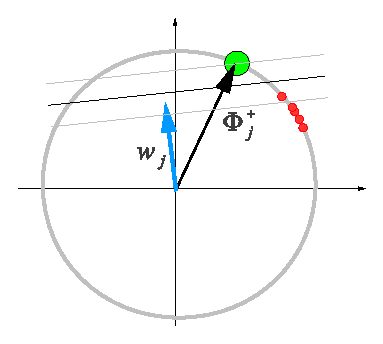
\includegraphics[trim = 4mm 0mm 7mm 3mm, clip=true, width=0.47\linewidth]{imgs/figSVM01tight}
            }
            %        $C_2 \rightarrow 0$
            \subfigure[$C_2 \rightarrow 0$]{
               \centering
               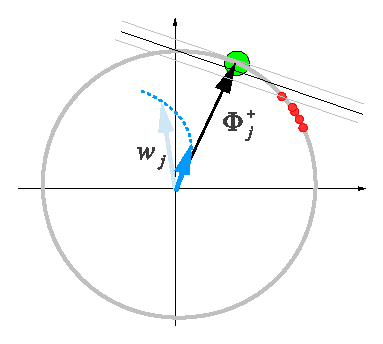
\includegraphics[trim = 3mm 0mm 8mm 3mm, clip=true, width=0.47\linewidth]{imgs/figSVM02tight}
            }
            \caption{
               {\bf An illustration of the effect of decreasing parameter $C_2$ in the exemplar support vector machine objective.} 
               The positive exemplar $\Phi_j^+$ is shown in green. The negative data points are shown in red. All training data is L2 normalized to lie on a hyper-sphere. (a) For $C_2>0$, the normal $w_j$ of the optimal hyper-plane moves away from the direction given by the positive example $\Phi^+$ in a manner that reduces the loss on the negative data.  (b) As the parameter $C_2$ decreases the learnt $w_j$ becomes parallel to the positive training example $\Phi_j^+$ and its magnitude $||w_j||$ goes to 0.
            }
            \label{fig:C2effect}
         \end{center}
      \end{figure}
      %
      \paragraph{Case I: $C_2\rightarrow 0$.}
         The goal is to show that when the weight  $C_2$ of the negative data in objective~\eqref{eq:obj} goes towards zero, the resulting hyperplane vector $w_j$ is parallel with the vector of positive training descriptor $\Phi_j^+$. When $w_j$ is normalized to have unit L2 norm the two vectors are identical. First, let us decompose $w$ into parallel and orthogonal part with respect to the positive training data point $\Phi^+$ (in the following we omit index $j$ for brevity), i.e. $w=w^{\perp}+w^{||}$, where $(w^{\perp})^T \Phi^+ = 0$. Next, we observe that when the weight of the negative data diminishes ($C_2\rightarrow 0$), any non-zero component $w^{\perp}$ will increase the value of the objective. As a result, for $C_2\rightarrow 0$ the objective is minimized by $w^{||}$, i.e.\ the optimal $w$ is parallel with $\Phi^+$.

         In detail, for $w=w^{\perp}+w^{||}$, the objective~(\ref{eq:obj}) can be written as
         %
         \begin{align}
            \label{eq:decomposedOrig}
              ||w^{\perp}+w^{||}||^{2} &+
              C_1 \cdot h
              \left(
               (w^{\perp}+w^{||})^T\Phi^+ + b
              \right) \\ \nonumber
              &+
              C_2\sum_{\Phi\in \mathcal N} h
              \left(
               -(w^{\perp}+w^{||})^T\Phi-b
              \right).
         \end{align}
         %
         Note that the orthogonal part $w^{\perp}$ does not change the value of  the second term in~(\ref{eq:decomposedOrig}) because $(w^{\perp}+w^{||})^T\Phi^+=(w^{||})^T\Phi^+$, and hence~(\ref{eq:decomposedOrig}) reduces to
         %
         \begin{align} 
            \label{eq:decomposed} 
            ||w^{\perp}+w^{||}||^{2} &+
            C_1 \cdot h
            \left(
                w^{||T}\Phi^+ +b_j
            \right) \\ \nonumber
            &+
            C_2\sum_{\Phi\in \mathcal N} h
            \left(
                -(w^{\perp}+w^{||})^T\Phi-b
            \right).
         \end{align}
         %
         In the limit case as $C_2 \rightarrow 0$ any non-zero component $w^{\perp}$
         will increase the value of the objective~\eqref{eq:decomposed}. This can be seen by noting that the third term vanishes when $C_2 \rightarrow 0$ and hence the objective is dominated by the first two terms. Further, the second term in~\eqref{eq:decomposed} is independent of $w^{\perp}$. Finally, the first term will always increase for any non-zero value of $w^{\perp}$ as $||w^{\perp}+w^{||}||^{2} \geq ||w^{||}||$ for any $w^{\perp}\neq0$.

         As a result, in the limit case when $C_2 \rightarrow 0$ the optimal $w$ is parallel with $\Phi^+$. Note also, that when $C_2$ is exactly equal to zero, $C_2=0$, the optimal $w$ vanishes, i.e. the objective~\eqref{eq:decomposed} is minimized by trivial solution $||w||=0$ and $b_j=-1$. The effect of decreasing the parameter $C_2$ is illustrated in figure~\ref{fig:C2effect}.


      \paragraph{Case II: $C_2>0$.}
         When the weight $C_2$ of the negative data in the objective~\eqref{eq:decomposed} increases the direction of the optimal $w$ will be different from $w^{||}$ and will change to take into account the loss on the negative data points. Explicitly writing the hinge-loss $h(x) = \max(1-x,0)$ in the last term of~\eqref{eq:decomposed}, we see that $w$ will move in the direction that reduces $\sum_{\Phi\in \mathcal N}\max \left(1+w^T \Phi + b ,0 \right)$, i.e.\ that reduces the dot product $w^T \Phi$ on the negative examples that are active (support vectors).


  %%%%%%%%%%%%%%%%%%%%%%%%%%%%%%%%%%%%%%%
  \section{Memory efficient classifier representation}  
  \label{sec:memory}
  %%%%%%%%%%%%%%%%%%%%%%%%%%%%%%%%%%%%%%% 
  % The method requires storing all the learnt classifiers w.
  % The optimal storage depends on the dimension and sparsity structure of w.
  % As will be discussed in detail section(exp), in this work we investigate two types of descriptors 
  % The high-dimensional sparse BOF and compact non-sparse FV.  
  % Some descriptors are dense. Some descriptors are sparse.
  
  %  For each image $j$, we learn a linear discriminative classifier with weight vector $\vec{w}_j$ and bias $b_j$.
  We learn a linear discriminative classifier with weight vector $\vec{w}_j$ and bias $b_j$ for each image $j$ in the database.   
  These classifier parameters become the new representation for each image. 
  %  This becomes the new representation for each image in the database. 
  In this section we discuss how the classifier parameters can be stored in a memory efficient manner that is amenable for indexing. 
  The goal is to apply all the learnt classifiers to the query descriptor $\vec{q}$
      %
      \begin{equation}
      \label{eq:allscores}
        \vec{s}=\vec{q}^T \mathcal{W}+\vec{b}, %=\vec{q}^T \mathcal{X}\cdot \mathcal{A}+\vec{b}
      \end{equation}
      %
  where $\mathcal{W}$ is $d\times N$ matrix storing all the learnt $\vec{w}_j$ classifiers as columns, $\vec{b}$ is a $1\times N$ vector storing all the learnt bias values $b_j$, 
  $\vec{q}$ is the input query descriptor, $\vec{s}$ is a $1\times N$ vector of output scores for all classifiers in the database, $N$ is the number of images in the database  and $d$ is the dimensionality of the image representation. 
  As discussed in detail in section~\ref{sec:experiments} we investigate two different image representations:  (i) the bag-of-visual-word vectors~\cite{Sivic03} and (ii) the compact Fisher vectors~\cite{Jegou12}. The learnt classifiers for these two image descriptors have different statistics and require different methods for storing and indexing. Next, we discuss the classifier representations for the two types of image representations.
 
  \paragraph{Bag-of-visual-words:}
    In the bag-of-visual-words representation, each image is represented by a high dimensional vector $\vec{x}$, where the dimensionality $d$ is typically $100,000$, but the vector is very sparse with only about 2,000 non-zero entries. 
    The learnt $\vec{w}_j$ are of the same (high) dimension $d$ but are {\em not sparse}. As a result, directly storing the learnt classifiers becomes quickly infeasible.
    To illustrate this, consider a database of $N=1,000,000$ images. Storing the original descriptors with about 2,000 non-zero entries for each image would take around 8GB. However, directly storing the learnt non-sparse $100,000\times 1,000,000 $ matrix $\mathcal{W}$ would require 400GB of memory. % for the same database.
    To address this issue we have developed an alternative indexing structure taking advantage of the dual form of the linear classifier as a sparse linear combination of a small number of support vectors~\cite{scholkopf2002learning}.   
    The key observation is that the number of support vectors $k$ is significantly lower then dimensionality $d$ of the original image descriptor. In the following we omit index $j$ for clarity.  In detail, we represent each $\vec{w}$ by its corresponding coefficients $\alpha_i$ of the linear combination of the support vectors (individual image descriptors) $\vec{x}_i$ such that
      %
      \begin{equation}
        \vec{w}=\sum_{i} \alpha_i \vec{x}_i = \mathcal{X} \cdot \vec{\alpha},
        \label{eq:dual}
      \end{equation}
      %
      \noindent
    where $\alpha_i$, the elements of vector $\vec{\alpha}$, are coefficients of the linear combination of the training data points $\vec{x}_i$ and the matrix $\mathcal{X}$ contains (as columns) descriptors of the entire database. Note that the vector $\vec{\alpha}$ is sparse and the number of non-zero elements depends on the number of support vectors $k$. 

   
    As a result, matrix $\mathcal{W}$ containing all learned classifier weights can be expressed in the dual form as
      %
      \begin{equation}
        \label{eq:dualFinal}
        \mathcal{W} = \mathcal{X} \mathcal{A},  
      \end{equation}
      %
    \noindent
    where $\mathcal{X}$ is the (sparse) matrix of the bag-of-visual-words image descriptors and $\mathcal{A}$ is the (sparse) matrix of $\alpha$ coefficients, 
    where each column corresponds to vector $\vec{\alpha}$ from \eqref{eq:dual}. Using this representation, the memory footprint is significantly reduced. Instead of storing all (non-sparse) weight vectors $\mathcal{W}$, which has memory complexity $O(dN)$ where $d$~(= 100,000) is the dimensionality of the image representation and $N$ is the size of the database, we store two sparse matrices $\mathcal{X}$ and $\mathcal{A}$, which has memory complexity $O(mN+kN)$ where $m$~(=2,000) is the number on non-zero elements in the original bag-of-visual-word descriptors, and $k$ is the typical number of support vectors. In our case $k$ is about the size of the training data which is around 500. As a result, the storage requirements are significantly reduced. For example, for a database of 1M images the dual representation requires only about 10 GB of storage compared to 400GB for directly storing classifiers $\mathcal{W}$.  
    Note that sparsity can be imposed directly on the learnt classifiers $\vec{w}$ by appropriate regularization~\cite{scholkopf2002learning}. However, we found this approach did not yield competitive results.


  \paragraph{Fisher vectors:}    
    The Fisher vector descriptors are not sparse and therefore the dual representation given by~\eqref{eq:dualFinal} does not bring any memory savings.
    However, they have a relatively low-dimension $d\in\{128, 512, 2048\}$ hence it is possible to store directly the (non-sparse) matrix $\mathcal{W}$ containing the learnt classifier parameters $\vec{w}$. In this work we exhaustively compute the classifier scores for all images in the database (given by equation~\eqref{eq:allscores}) using efficient (but exact) matrix-vector multiplication routines. However, this computation can be further sped-up using product quantization indexing as described in~\cite{Jegou12}.     



%%%%%%%%%%%%%%%%%%%%%%%
\section{Experimental setup and implementation details}
\label{sec:experiments}
%%%%%%%%%%%%%%%%%%%%%%%
  In this section we describe the experimental datasets, outline the two types of used image descriptors, and finally give implementation details of the classifier learning procedure.
  

  %%%%%%%%%%%%%%%%%%%%%%%%%%
  \subsection{Image datasets}
  %%%%%%%%%%%%%%%%%%%%%%%%%%
    \paragraph{Image database.}
      We performed experiments on a database of Google Streetview images from the Internet. We downloaded panoramas from Pittsburgh (U.S.) covering roughly an area of $1.3 \times 1.2 \; {\rm km}^2$. Similar to~\cite{Chen11}, we generate for each panorama 12 overlapping perspective views corresponding to two different elevation angles $4^\circ$ and $28^\circ$ to capture both the street-level scene and the building fa\c{c}ades. This results in a total of 24 perspective views each with $90^\circ$ FOV and resolution of $960 \times 720$ pixels. In this manner we generate two datasets. The first smaller dataset covers a smaller area and contains $25$k perspective images. The second larger dataset contains $55$k images.

      \paragraph{Query set.}
      As a query set with known ground truth GPS positions, we use 8999 panoramas from the Google Streetview research dataset, which cover approximately the same area, but were captured at a different time, and typically depict the same places from different viewpoints and under different illumination conditions.          
      We generate a test query set such that we, first select a panorama at random and, second, we generate a perspective image with a random orientation and random elevation pitch. This way we synthesize 4,000 query test images.


      \subsection{San Francisco dataset}
      \textcolor{petr}{
      We do not perform our experiments on the San Francisco dataset~\cite{Chen11} because it uses different definition of a ground truth. The ground truth of the San Francisco dataset is based on Geographic Information System (GIS). Each database and query image has associated cartographic ID based on what building is captured on it. As a result, the ground truth for particular query image often contains database images that are spatially far away ($> 200m$) from the query location.  However, our method defines ground truth images as those within a threshold of $20m$ from the query location and defines potential hard negatives images as those above the threshold of $200m$. As a consequence, our method identifies the ground truth images from San Francisco as hard negatives examples and uses them for training which dramatically affects the performance.
      }

    %%%%%%%%%%%%%%%%%%%%%%%%%%
    \subsection{Image descriptors}
    %%%%%%%%%%%%%%%%%%%%%%%%%%
      We perform experiments with two types of image descriptors: the sparse high-dimensional bag-of-visual-word vectors~\cite{Sivic03} and the compact (not-sparse) Fisher vectors~\cite{Jegou12}. Details of each are given next.

      \paragraph{Bag-of-visual-word representation.}
         We extract SURF descriptors~\cite{Bay06} for each image and learn a vocabulary of $100$k visual words by approximate k-means clustering~\cite{Philbin07} from a subset of features from $5,000$ randomly selected database images. Then, a tf-idf weighted vector~\cite{Sivic03} is computed for each image by assigning each descriptor to the nearest cluster center.  Finally, all database vectors are normalized to have unit $L_2$ norm.
        
      \paragraph{Fisher vectors.}
        Following~\cite{Jegou12} we project the extracted 128-dimensional rootSIFT~\cite{Arandjelovic12} descriptors to 64 dimensions using PCA. The projection matrix is learnt on a set of descriptors from 5,000 randomly selected database images. This has also the effect of decorrelating the rootSIFT descriptor. The 64-dimensional descriptors are then aggregated into Fisher vectors using a Gaussian mixture model with $N=256$ components, which results in a $2\times256\times64 = 32,768$-dimensional descriptor for each image.  
        The Gaussian mixture model is learnt from descriptors extracted from 5,000 randomly sampled database images. The  high-dimensional Fisher vector descriptors are then projected down to dimension $d\in\{128,512, 2048\}$ using PCA learnt from all available images in the database. The resulting low dimensional Fisher vectors are then-normalized to have unit L2-norm, which we found to be important in practice.
      
    %%%%%%%%%%%%%%%%%%%%%%%%%%
    \subsection{Parameters of per-location classifier learning}
    %%%%%%%%%%%%%%%%%%%%%%%%%%
      To learn the exemplar support vector machine for each database image $j$, the positive and negative training data are constructed as follows. 
      The \emph{negative training set} $\mathcal N_j$ is obtained by: (i) finding the set of images with geographical distance greater than $200{\rm m}$; (ii)  sorting the images by decreasing value of similarity to image $j$ measured by the dot product between their respective descriptors; (iii) taking the top $N=500$ ranked images as the negative set. 
      In other words, the negative training data consists of the hard negative images, i.e. those that are similar to image $j$ but are far away from its geographical position, hence, cannot have the same visual content. 
      The \emph{positive training set} $\mathcal P_j$ consist of the descriptor $\vec{x}_j$ of the target image $j$. 
      We found that for the bag-of-visual-words representation it was useful to further expand~\cite{Chum07b} positive training set by few (1-5) close by images that view the same scene structures. These images can be identified by geometric verification \cite{Philbin07}.   

      For the support vector machine classifier (SVM) training we use {\tt libsvm} \cite{libsvm}. We use the same $C_1$ and $C_2$ parameters for all per-exemplar classifiers, but find the optimal value of the parameters for each image representation by a cross-validation evaluating performance on a held out query set.

      For the calibration by re-normalization, we $L_2$ normalize the learned $\vec{w}_j$ using equation~\eqref{eq:linear3} and use this-normalized vector as the new image descriptor $\vec{x}'_j$ for image $j$. At query time we compute the descriptor $\vec{q}$ of the query image and measure its similarity score to the learnt descriptors $\vec{x}'_j$ for each database image by equation~\eqref{eq:class}.

      For the p-value calibration, we take the learnt classifier for each database image $j$ and compute its SVM score for all other database images to construct its empirical cumulative density function~\eqref{eq:empiricalCDF}. We keep only the top 1,000 values that, in turn, represent the calibration function. At query time, given the query descriptor $\vec{q}$, we compute the SVM score~\eqref{eq:linear} for each database image $j$, and compute its calibrated SVM score $f_j$~\eqref{eq:empiricalCDF}.


%%%%%%%%%%%%%%%%%%%%
\section{Results}
\label{sec:results}
%%%%%%%%%%%%%%%%%%%%
  We evaluate the proposed per-location classifier learning approach on two different image descriptors: the bag-of-visual-words model (section~\ref{sec:bow_results} ) and Fisher vectors (section~\ref{sec:fisher_restuls}).  Finally, we compare the recognition accuracy of the two learnt representations relative to their compactness measured by their memory footprint (section~\ref{sec:memory_results}).
%  Finally, we also evaluate the dependence of the recognition accuracy on the memory requirements (section~\ref{sec:memory_results}).
  % and finally report qualitative results  (section~\ref{sec:qualitative_results}).   
  Since the ground truth GPS position for each query image is available, for each method we measure performance using the percentage of correctly recognized queries (Recall) similarly to, e.g.,~\cite{Chen11,Knopp2010,Sattler-BMVC12}. We deem the query as correctly localized if at least one of the top $K$ retrieved database images is within $20$ meters from the ground truth position of the query. 


  %%%%%%%%%%%%%%%%%
  \subsection{Bag-of-visual-words model}
  \label{sec:bow_results}
  %%%%%%%%%%%%%%%%%
  
    %%% TABLE: Results 25k BOW only
    \begin{table}[tbp]
      \begin{centering}
        
	\begin{tabularx}{0.915\linewidth}{|l|c c c c c|}
		\hline 
		\rowcolor{maroon!50}
		Method: & \multicolumn{5}{c|}{25k Pittsburgh} \\
		\hline 
		\hline 
		%%%%%%%%%%%%%%%%%%%%%%%%%%%%%%%%%%%%%%%%%%%%%%%%%%%%%%%%%%%%%%%%%%%%%%%%%%%%
		\rowcolor{maroon!50}
		recall@K [$\%$] & 1 & 2 & 5 & 10 & 20 \\
		\hline
		\rowcolor{maroon!10}
      \rowcolor{maroon!10}
    BOW SVM no calib.   & 6.4   & 8.1   & 13.5  & 17.5  & 20.5 \\
		  \rowcolor{maroon!10}
    BOW           & 28.7  & 35.7  & 45.8 & 53.7   & 61.5 \\
      \rowcolor{maroon!10}
    
    \textcolor{petr}{BOW  Knopp[]}  & \textcolor{petr}{29.6}  & \textcolor{petr}{37.3}  & \textcolor{petr}{48.9} & \textcolor{petr}{59.3}   & \textcolor{petr}{69.2}  \\
      \rowcolor{maroon!10}
		BOW w-norm  & 31.8    & 38.7  & 49.7  & \textbf{60.2}  & \textbf{69.4} \\
      \rowcolor{maroon!10}
    BOW p-val     & \textbf{33.0}  & \textbf{40.3}  & \textbf{50.2} & 58.7   &  66.4 \\
    \hline
  %   %%%%%%%%%%%%%%%%%%%%%%%%%%%%%%%%%%%%%%%%%%%%%%%%%%%%%%%%%%%%%%%%%%%%%%%%%%%%
		% \rowcolor{maroon!10}
		% FV128         & 33.6  & 41.8  & 52.0 & 59.8   & 67.7  \\
		% \rowcolor{maroon!10}
		% % FV128 p-val                 & \textbf{}       & \textbf{}     & \textbf{}     & \textbf{}     & \textbf{}  \\
  % %   \rowcolor{maroon!10}
		% \textbf{FV128 w-norm}     & \textbf{38.3}   & \textbf{47.5} & \textbf{57.7} & \textbf{65.8} & \textbf{72.7}  \\
  %   \hline  
  %   %%%%%%%%%%%%%%%%%%%%%%%%%%%%%%%%%%%%%%%%%%%%%%%%%%%%%%%%%%%%%%%%%%%%%%%%%%%%%
  %   \rowcolor{maroon!10}
  %   FV512         & 44.3 & 51.7   & 61.4  & 68.7   & 75.2  \\
  %   \rowcolor{maroon!10}
  %   \textbf{FV512 w-norm}   & \textbf{47.6}  & \textbf{55.4} & \textbf{65.1} & \textbf{72.4} & \textbf{78.8}  \\
  %   \hline
  %   %%%%%%%%%%%%%%%%%%%%%%%%%%%%%%%%%%%%%%%%%%%%%%%%%%%%%%%%%%%%%%%%%%%%%%%%%%%%%%
		% \rowcolor{maroon!10}
		% FV2048        & 46.9  & 54.1  & 63.8  & 70.5    & 76.8 \\
		% \rowcolor{maroon!10}
		% % FV2048 p-val  & \textbf{} & \textbf{} & \textbf{} & \textbf{} & \textbf{} &
  % %       \textbf{} & \textbf{} & \textbf{} & \textbf{} & \textbf{}\\
  %       \rowcolor{maroon!10}
  %       \textbf{FV2048 w-norm}  & \textbf{50.2} & \textbf{57.3} & \textbf{67.0} & \textbf{73.8} & \textbf{78.0} \\
  %       \hline
  %       %%%%%%%%%%%%%%%%%%%%%%%%%%%%%%%%%%%%%%%%%%%%%%%%%%%%%%%%%%%%%%%%%%%%%%%%%%%%%%%%
  % %       \rowcolor{maroon!10}
  % %       FV8192        & 46.0  & 52.7 & 62.5 & 69.4 & 76.4 & - & - & - & - &  -   \\
  % %       \rowcolor{maroon!10}
  % %       \textbf{FV8192 w-norm}  & \textbf{48.4} & \textbf{55.6} & \textbf{65.4} & \textbf{72.6} & \textbf{79.0} & - & - & - & - & -\\
		% % \hline
\end{tabularx}

        \caption{ 
          \textbf{Evaluation of the learnt bag-of-visual-words representation on the Pittsburgh 25k dataset.}
          The table shows the fraction of correctly recognized queries (recall@K) for the different values of $K\in\{1,2,5,10,20\}$ retrieved database images. 
          The learnt representations (BOW w-norm and BOW p-val) outperform the raw bag-of-visual-words baseline (BOW) as well as the learnt representation without calibration (BOW SVM no calib).  
        }
        \label{tab:recallBOW}
      \end{centering}
    \end{table}

    %%% PLOT: BOW recall curves
    \begin{figure}[tbp]
        \centering
        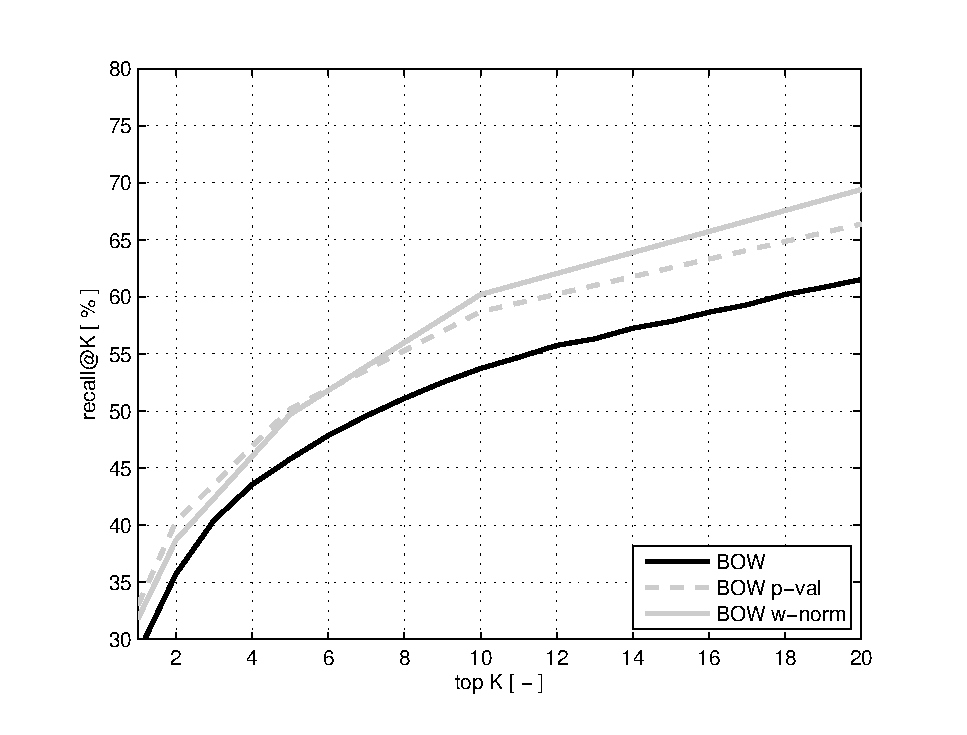
\includegraphics[width=1.1\linewidth]{imgs/plotPitt25kBOW}  
        %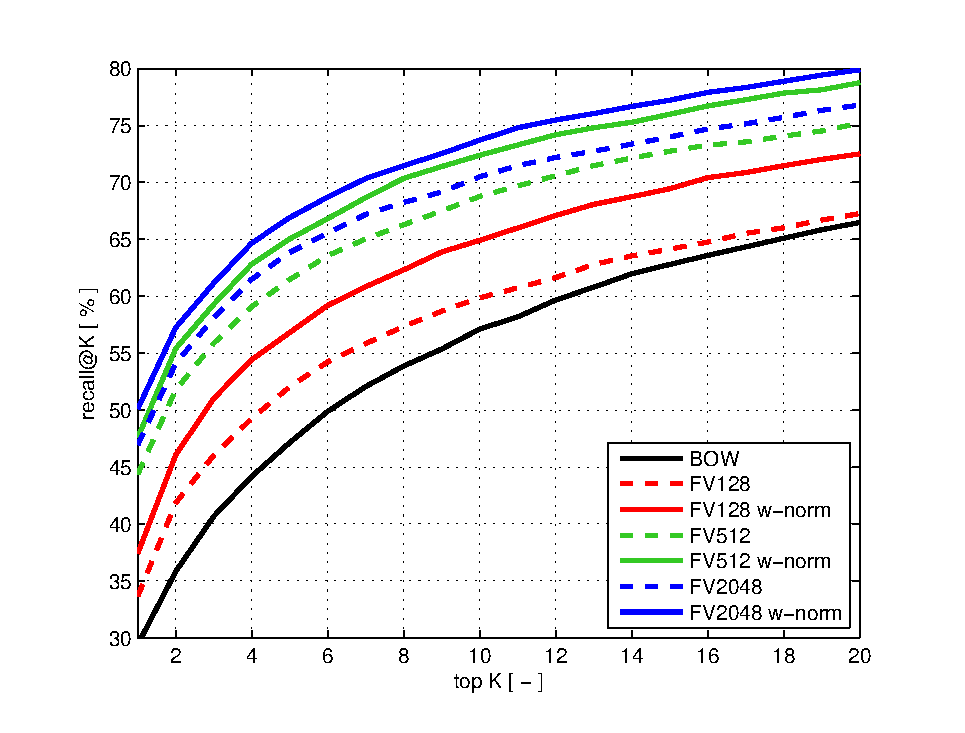
\includegraphics[trim=35mm 70mm 40mm 75mm, clip=true, width=\linewidth]{imgs/plotPitt25k}    
        \caption{
            % \textbf{TODO: Evaluation of the learnt Fisher vector representation on the Pittsburgh 25k \cite{Gronat13} dataset.} 
            % The graph shows the fraction of correctly recognized queries (recall@K, y-axis) vs. the number of top $K$ retrieved database images for the raw Fisher vector baseline (FV) for different dimensions compared to the learnt representation (w-norm). Note the consistent improvements over all lengths of shortlist $K$ for all dimensions.
            \textbf{Evaluation of the learnt bag-of-visual-words representation on the Pittsburgh 25k \cite{Gronat13} dataset.} The graph shows the fraction of correctly recognized queries (recall@K, y-axis) vs. the number of top $K$ retrieved database images for the raw bag-of-visual-words baseline (BOW) and the learnt representation with two different calibration methods (p-val and w-norm).
        }
        \label{fig:recallBOW}
    \end{figure}

    Results for the bag-of-visual-words image representation are shown in table~\ref{tab:recallFV}. %  and figure~\ref{fig:recallBOW}. 
    Learning per-location classifiers with either calibration method (\emph{p-val} and \emph{w-norm}) clearly improves over the standard bag-of-visual-words baseline (BOW) that does not perform any learning. In addition, both calibration methods significantly improve over the learnt SVM classifiers without any calibration (BOW SVM no calib) underscoring the importance of calibration for the independently learnt per-location classifiers.  
    Inspecting the detailed plots in figure~\ref{fig:recallBOW} we further note that the  \emph{p-val} calibration performs slightly better than the \emph{w-norm} calibration for shorter top $K$ shortlists but this effect is reversed for larger $K$. This could be attributed to the fact that the \emph{p-val} calibration uses the negative data to control false positive errors, but has less control over false negatives, as discussed in section~\ref{sec:discussion}. 

    In figure~\ref{fig:3qVSw} we visualize the learnt SVM weights on BOW for \emph{p-val}. We visualize the contribution of each feature to the SVM score for the corresponding query image. Red circles represent features with negative weights while green circles correspond to features with positive weights. The area of each circle is proportional to the contribution of the corresponding feature to the SVM score. For instance for the left figure notice that the correctly localized queries (c) contain more green colored features than queries from other places (b) and (a). Query (b) gets a high score because the building has orange and white stripes similar to the the sun-blinds of the bakery, which are features that also have large positive weights in the query image (c) of the correct place.
    In the top row we visualize the calibration of raw SVM score for three different queries. The calibration function of the target image $j$ is shown in the blue and the corresponding SVM scores of the three queries are denoted by red circles. Notice that both images (b) and (c) have high calibrated score even their respective SVM score was different.     
    
    Finally, examples of correctly and incorrectly localized queries are shown in figure~\ref{fig:images_bow}. 
%    The query image is show in the left column and the shortlist of the top four retrieved images is shown on the right. For each query, the first row shows images retrieved by the learnt bag-of-visual-words descriptor, while the second row shows images retrieved by the raw bag-of-visual-words descriptor without place specific learning.

    %%% FIGURE: Visualization of removed visual words
  \begin{figure*}[tbp]
      \begin{figure*}%[tbp]
  \begin{minipage}{0.48\linewidth}
          \begin{minipage}{0.65\linewidth}
            \centering
            {\scriptsize Calibrated classifier score $f_j$}
            \\
            \vspace{2mm}
            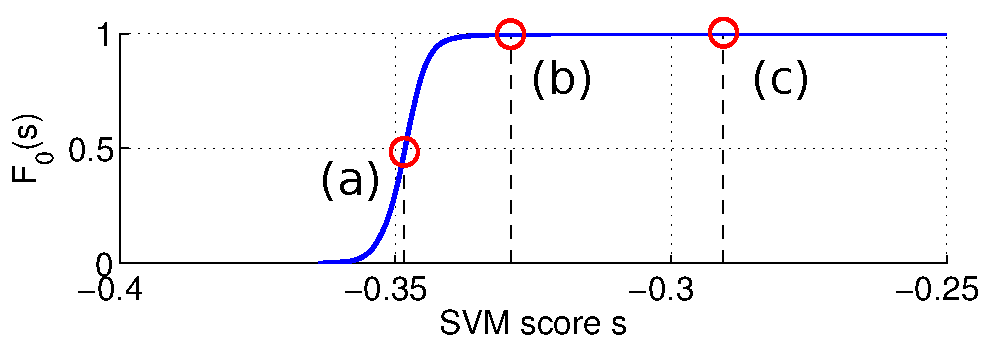
\includegraphics[width=\linewidth]{imgs/wVS3q/2882/graphBigO.pdf}
          \end{minipage} 
          %
          \begin{minipage}{\wii}
            \centering
            \centerline{\scriptsize Target database image $j$}
            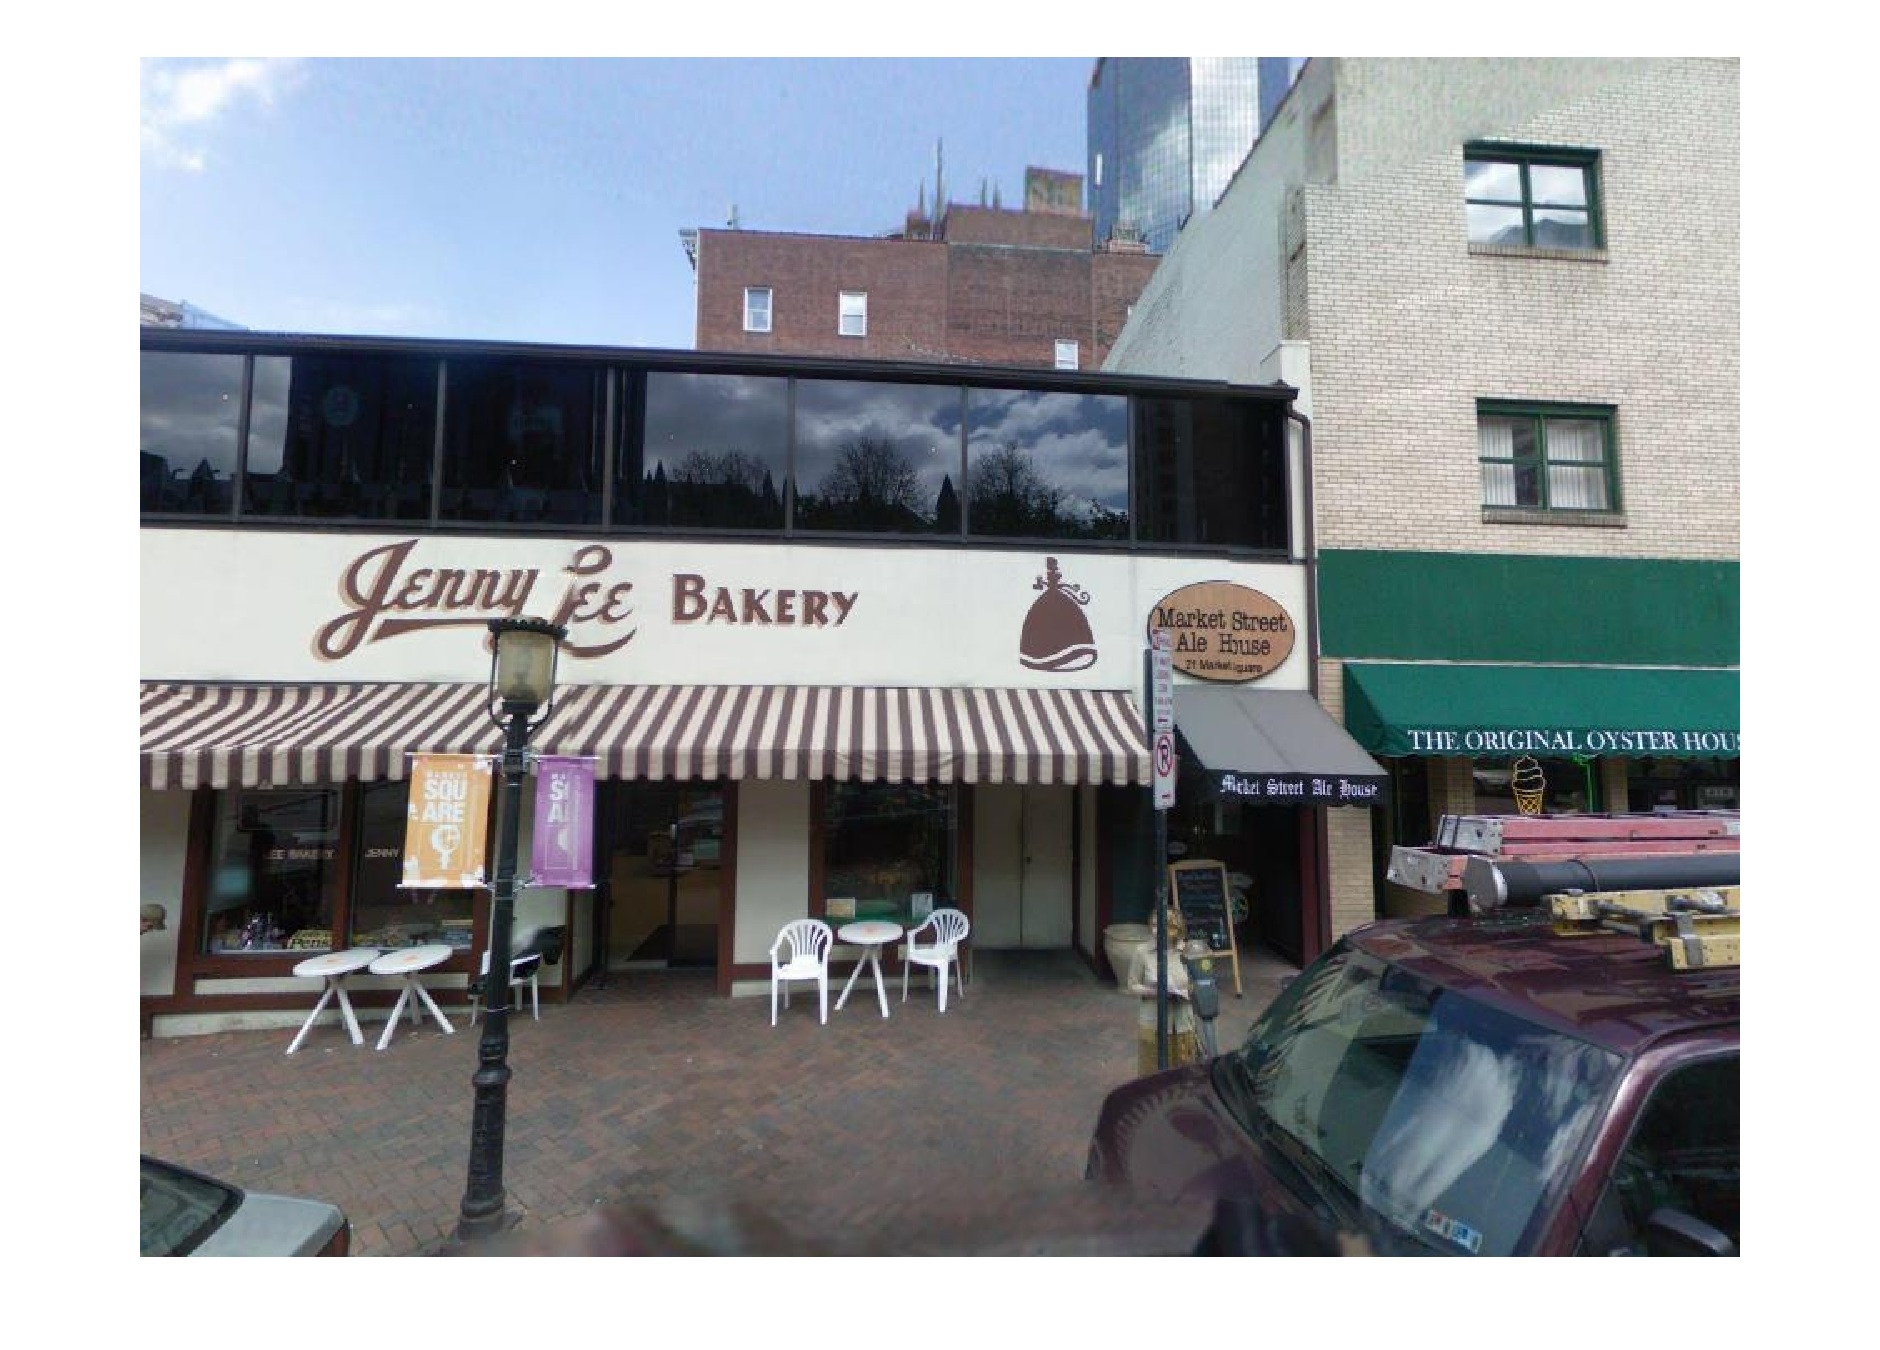
\includegraphics[width=\linewidth]{imgs/wVS3q/2882/j.jpg}
          \end{minipage}  
          \vspace{3mm}
          \\
          \centerline{\scriptsize Classified query images $f_j(q)$} 
          \\
          \begin{minipage}{\wii}
            \centering
            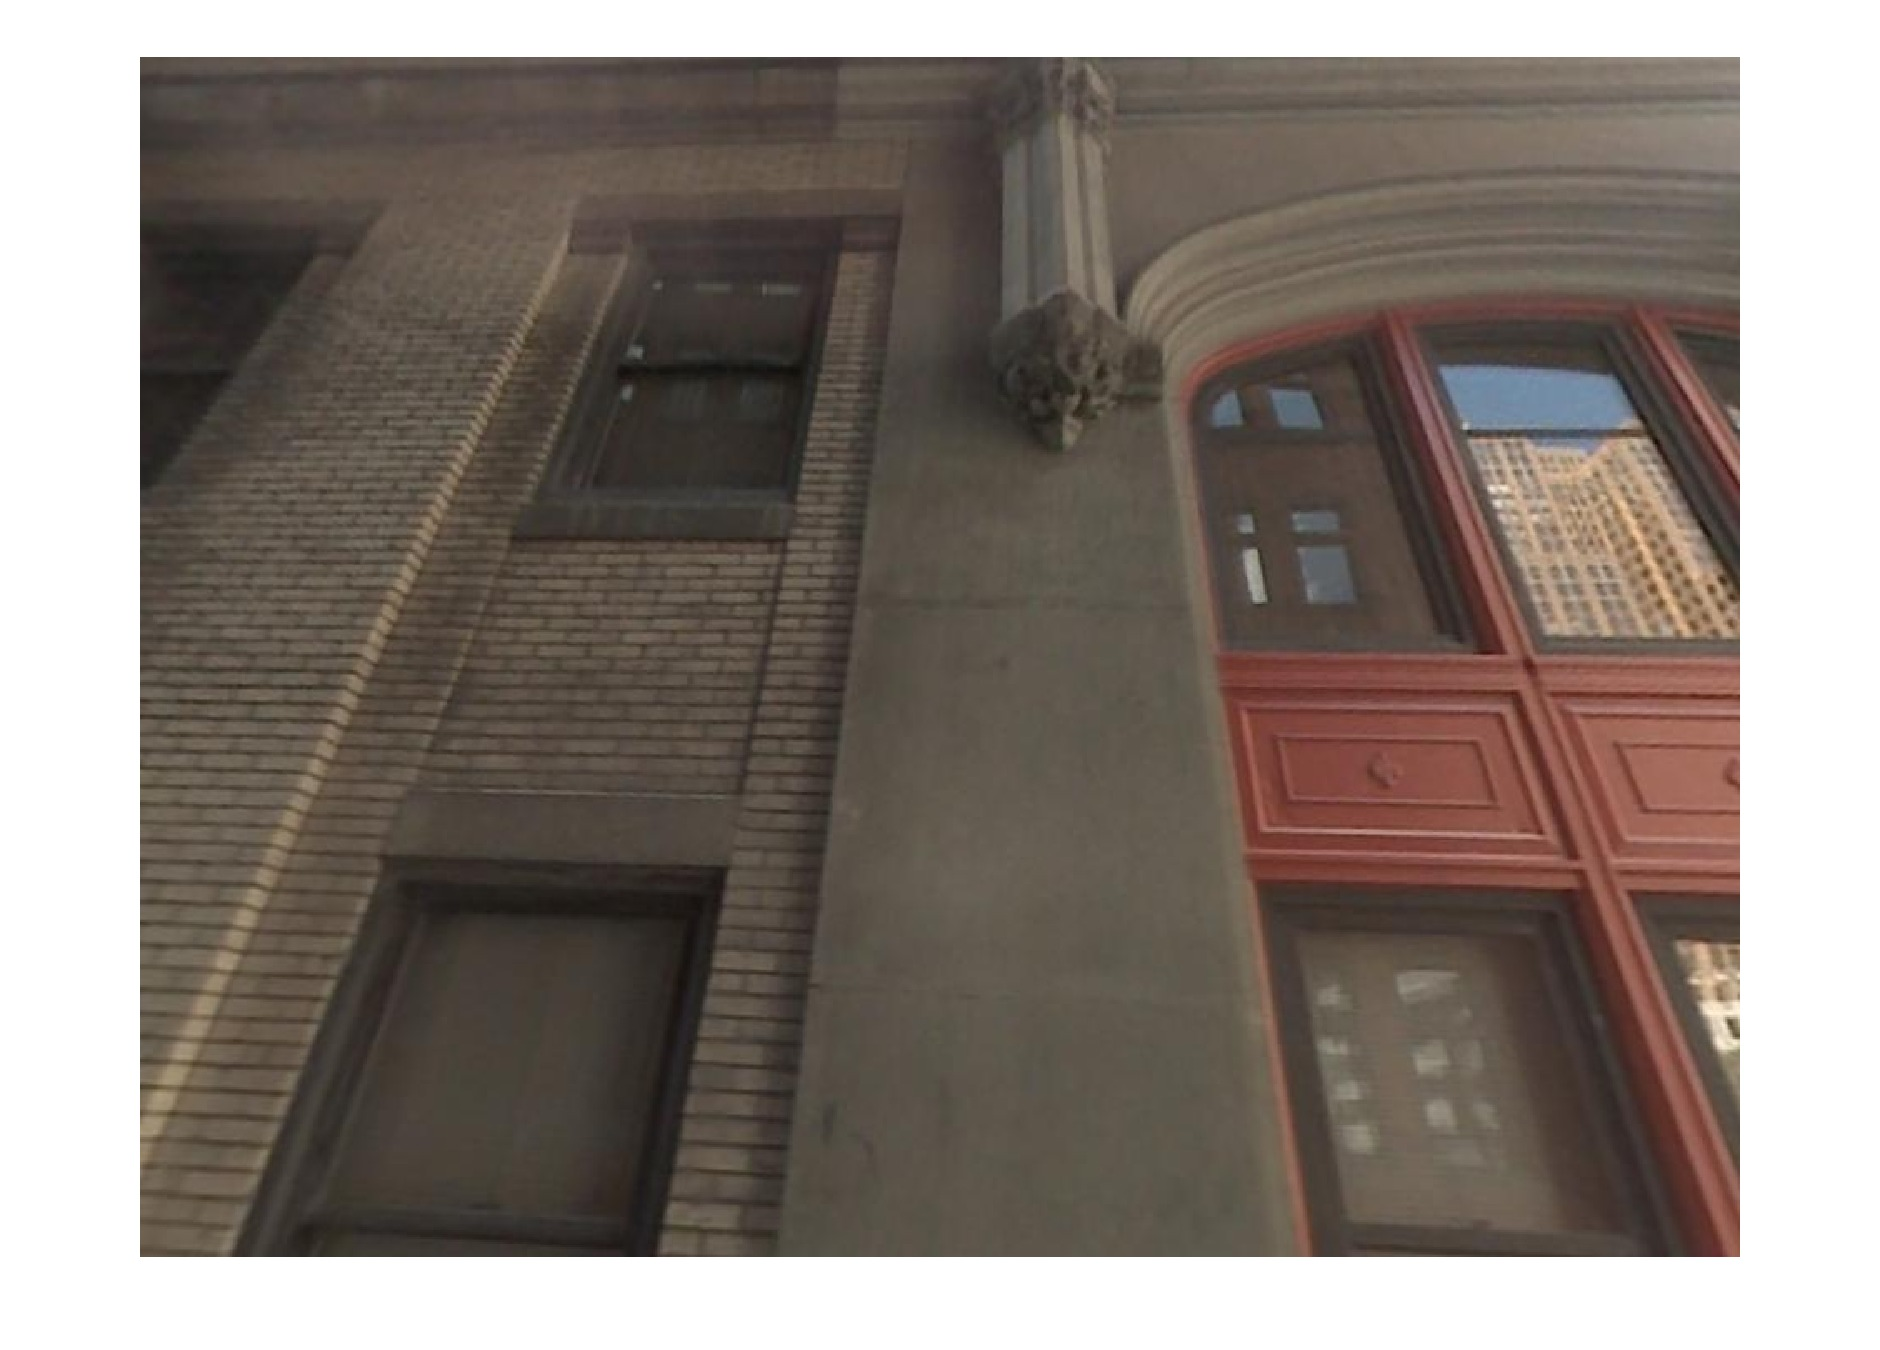
\includegraphics[width=\linewidth]{imgs/wVS3q/2882/a.jpg}
          \end{minipage}
          %  
          \begin{minipage}{\wii}
            \centering
            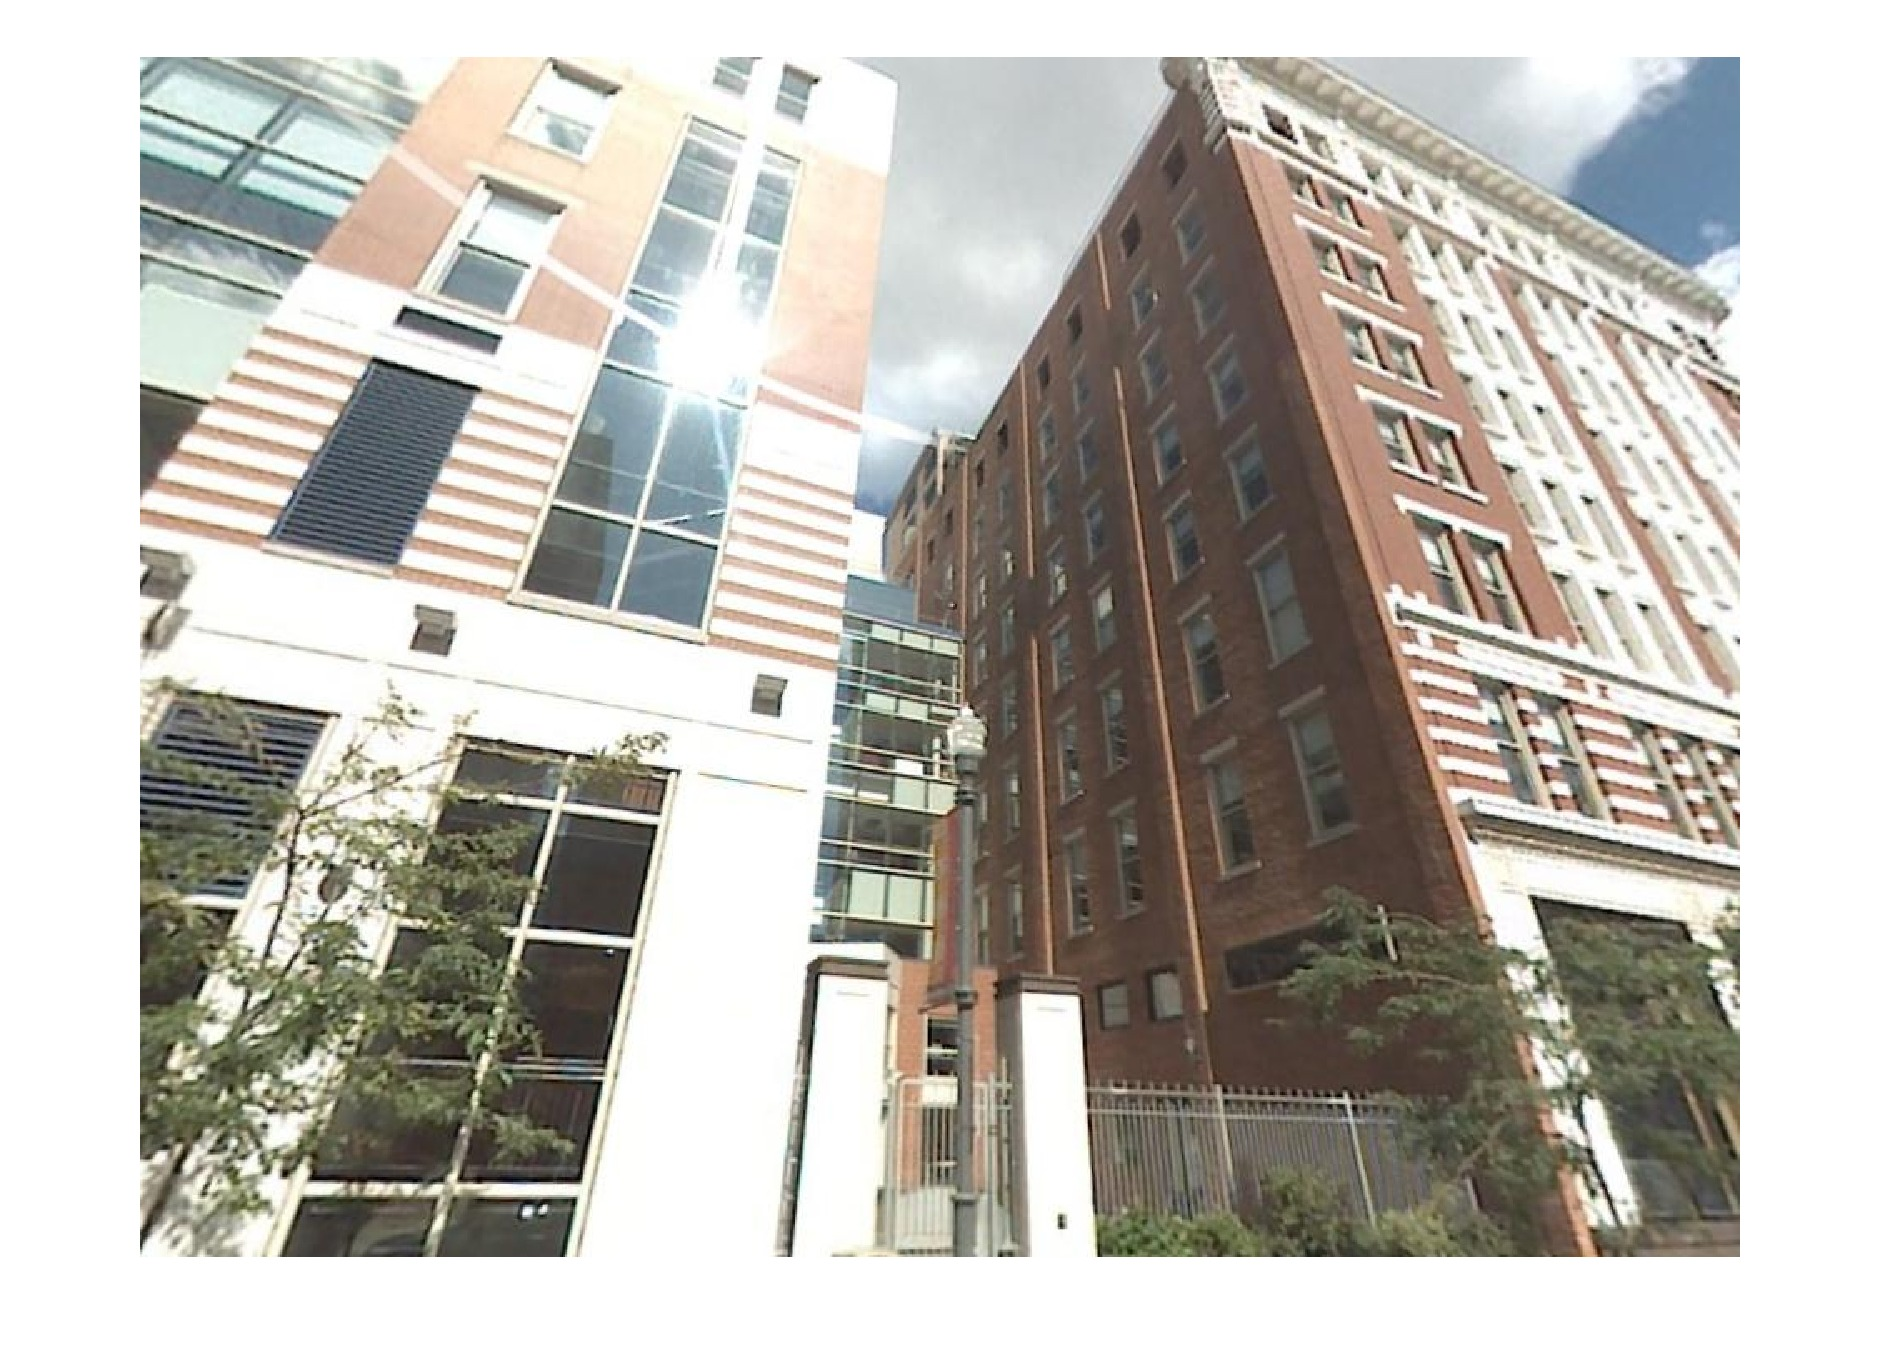
\includegraphics[width=\linewidth]{imgs/wVS3q/2882/b.jpg}
          \end{minipage}
          %  
          \begin{minipage}{\wii}
            \centering
            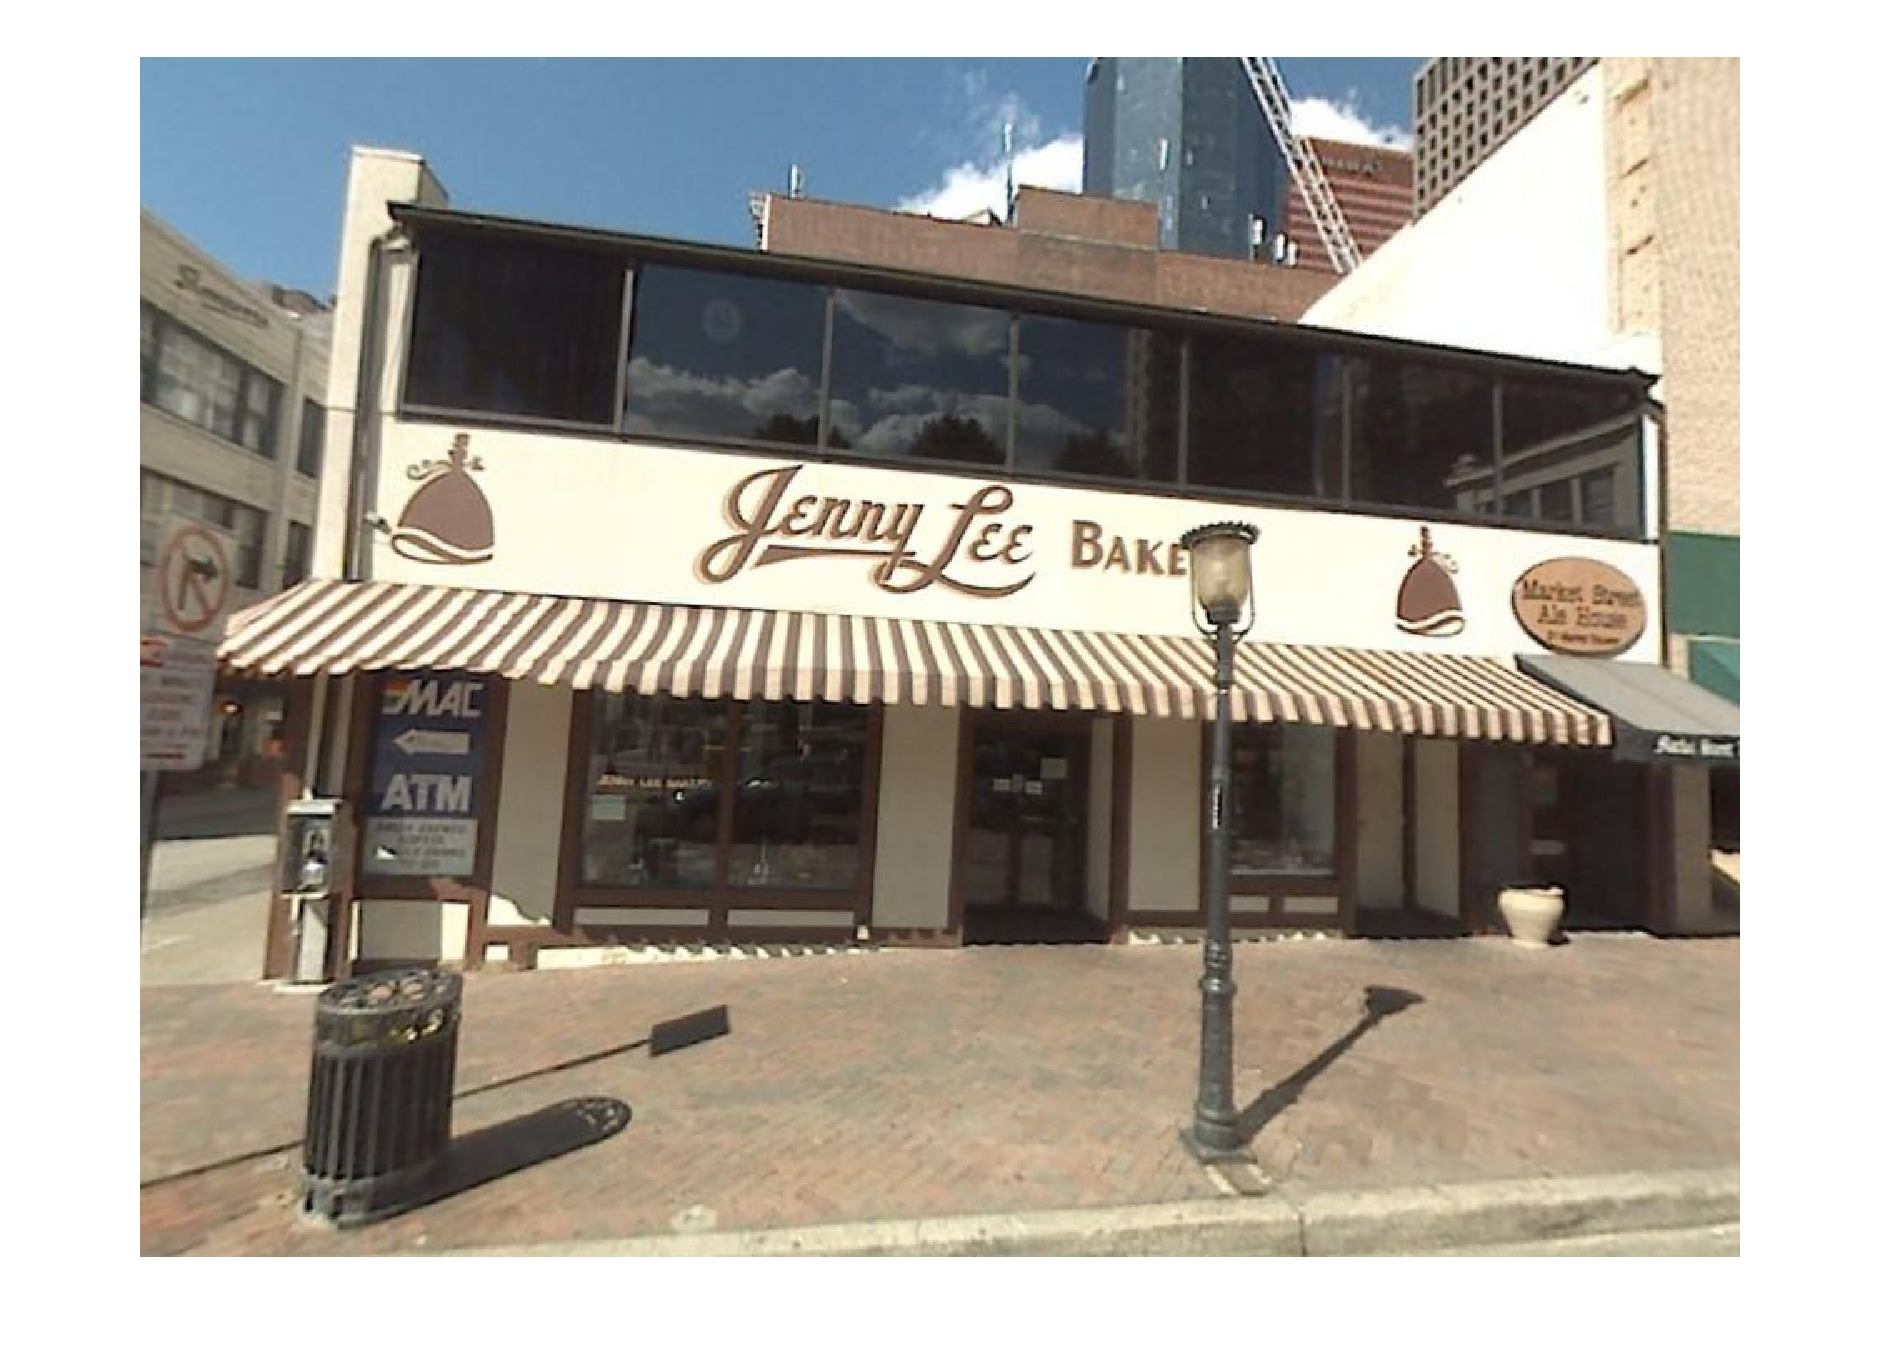
\includegraphics[width=\linewidth]{imgs/wVS3q/2882/c.jpg}
          \end{minipage} 
          \\
          \begin{minipage}{\wii}
            \centering
            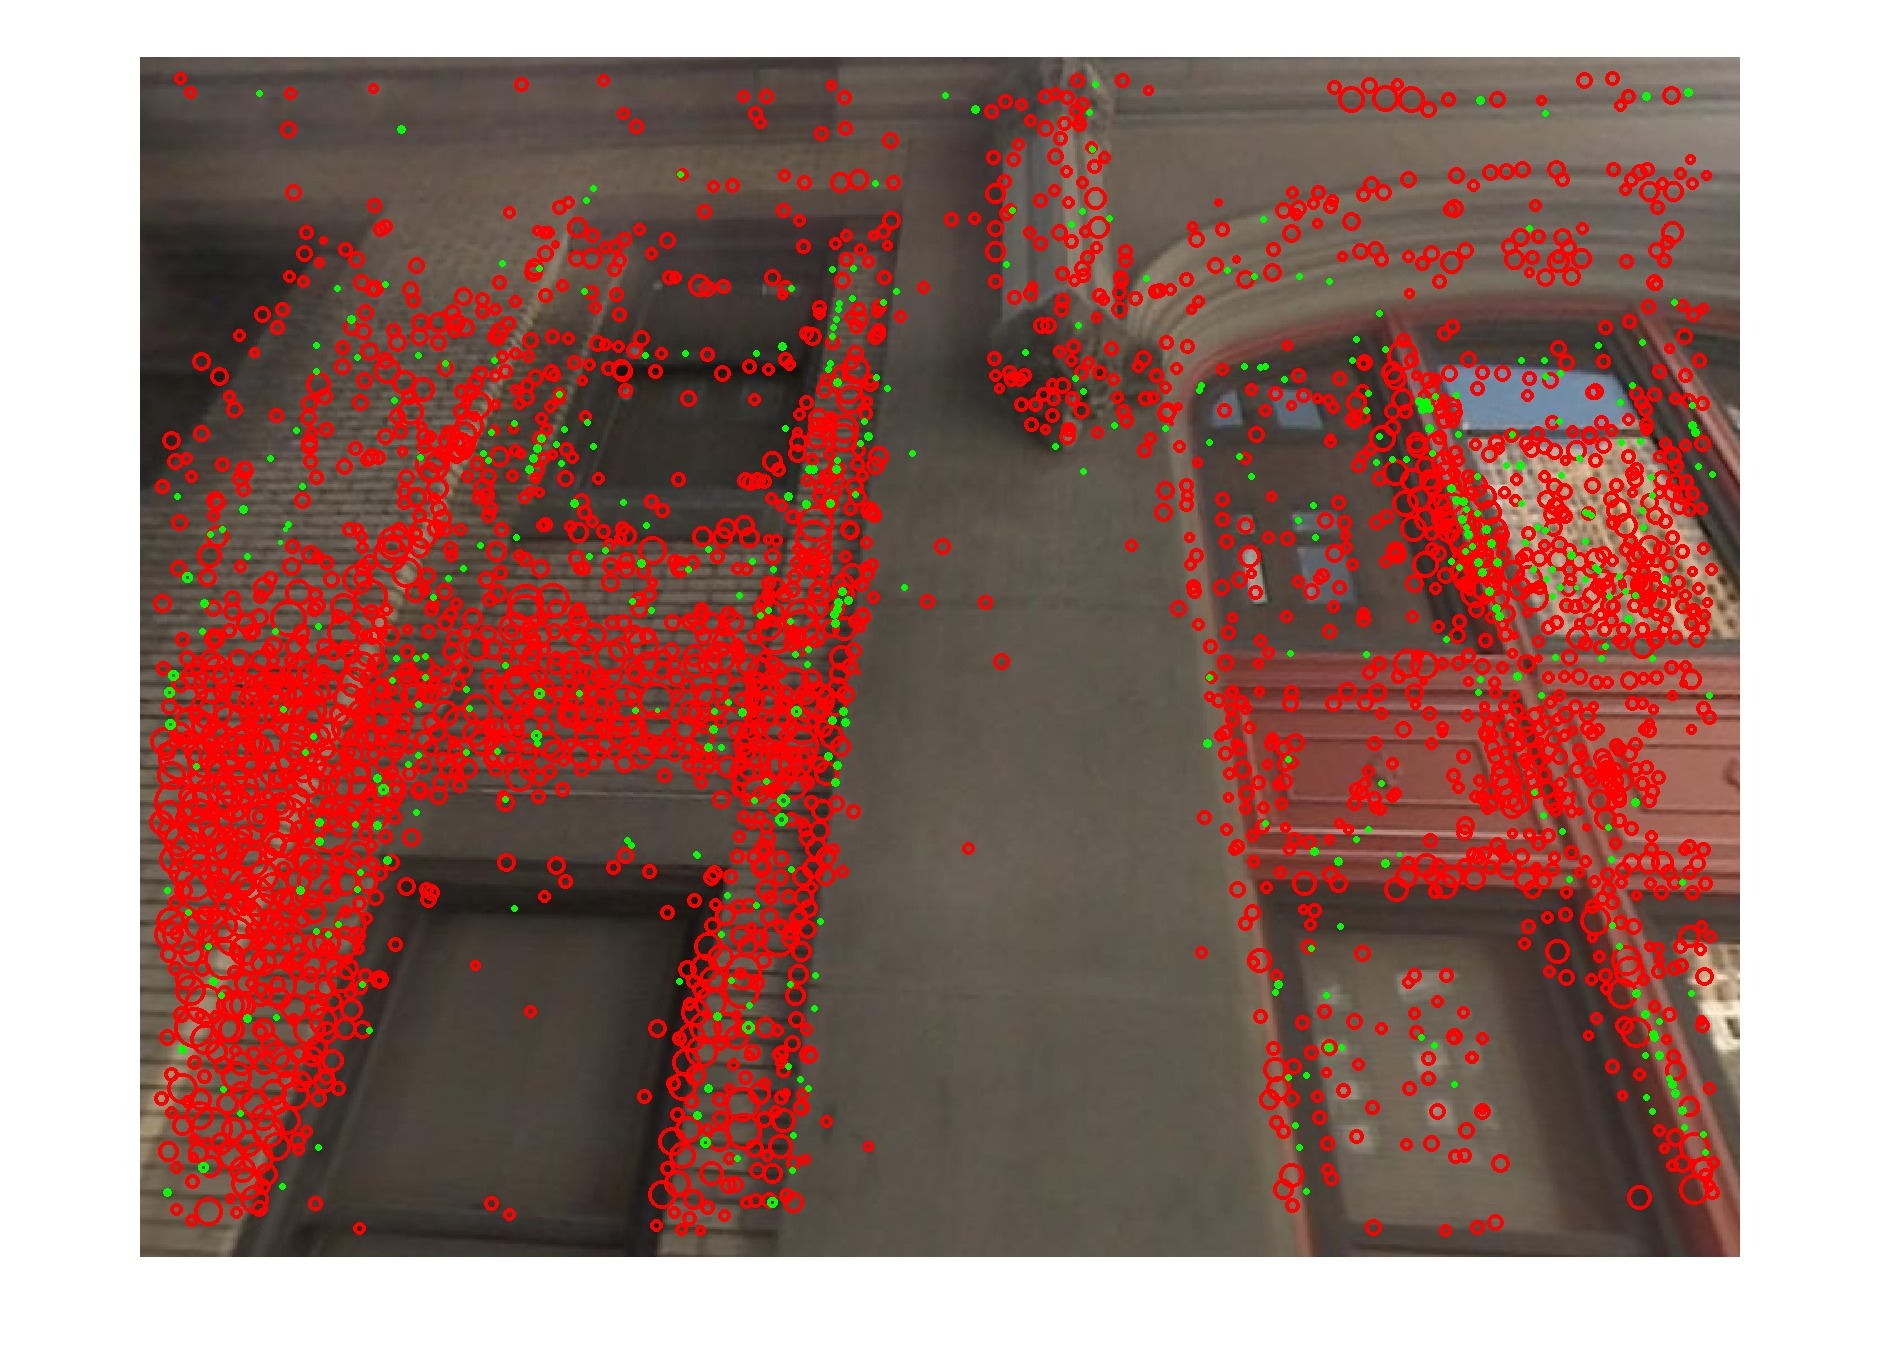
\includegraphics[width=\linewidth]{imgs/wVS3q/2882/aftrs.jpg}
            \newline
            (a)
          \end{minipage}  
          \begin{minipage}{\wii}
            \centering
            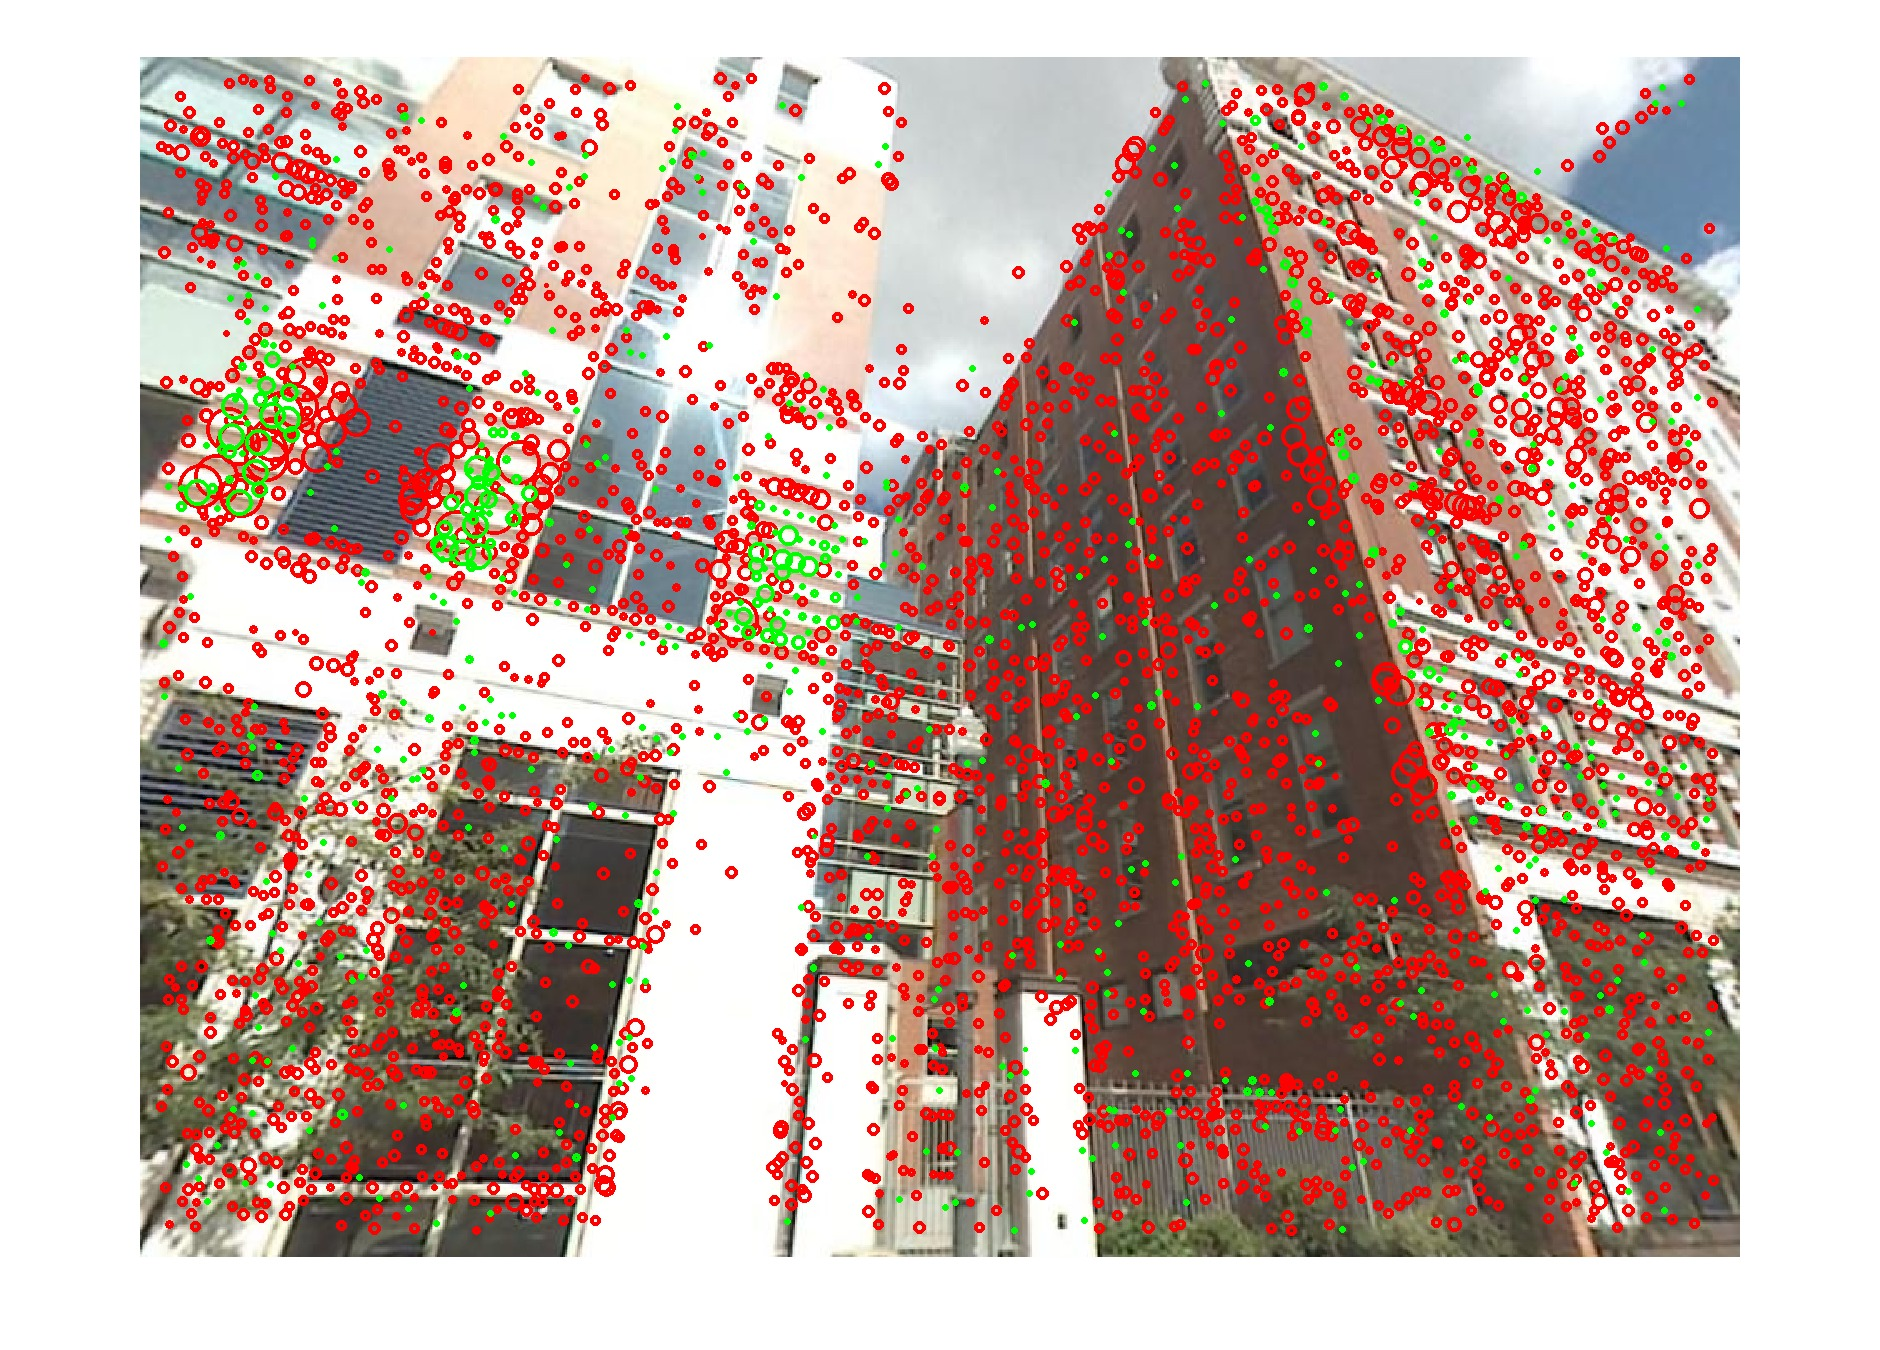
\includegraphics[width=\linewidth]{imgs/wVS3q/2882/bftrs.jpg}
            \newline
            (b)
          \end{minipage}  
          \begin{minipage}{\wii}
            \centering
            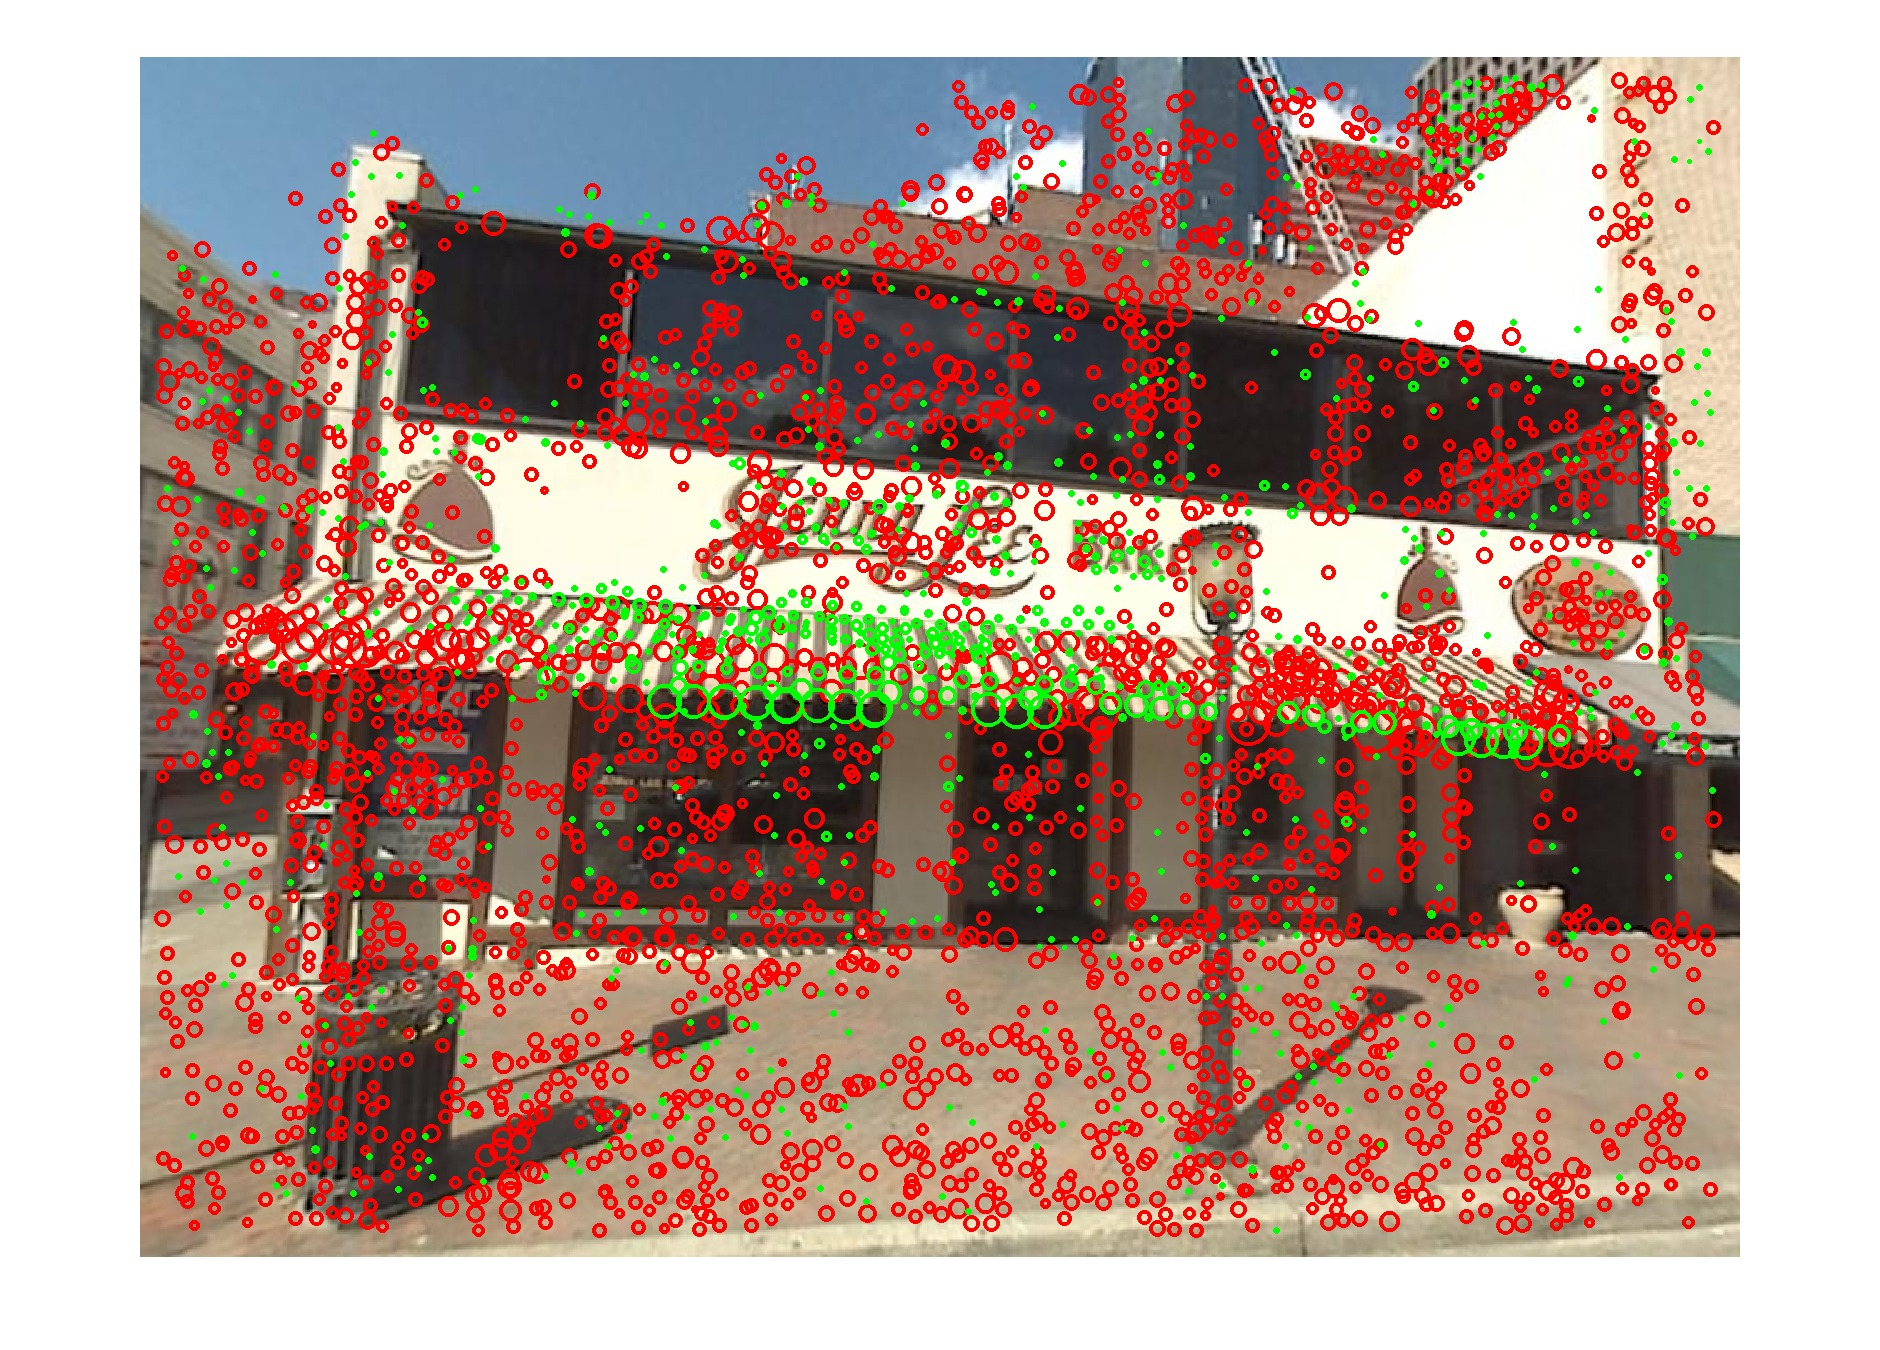
\includegraphics[width=\linewidth]{imgs/wVS3q/2882/cftrs.jpg}
            \newline
            (c)
          \end{minipage} 
    \end{minipage}% left figure
    %
    %%%%%%%%%%%%%%%%%%%%%%%%%%%%%%%%%
    \begin{minipage}{0.04\linewidth}
      \hspace{\linewidth}
    \end{minipage}
    %%%%%%%%%%%%%%%%%%%%%%%%%%%%%%%%%
    % RIGHT FIGURE
    \begin{minipage}{0.48\linewidth}
          \begin{minipage}{0.66\linewidth}
            \centering
            {\scriptsize Calibrated classifier score $f_j$}
            \\
            \vspace{2mm}
            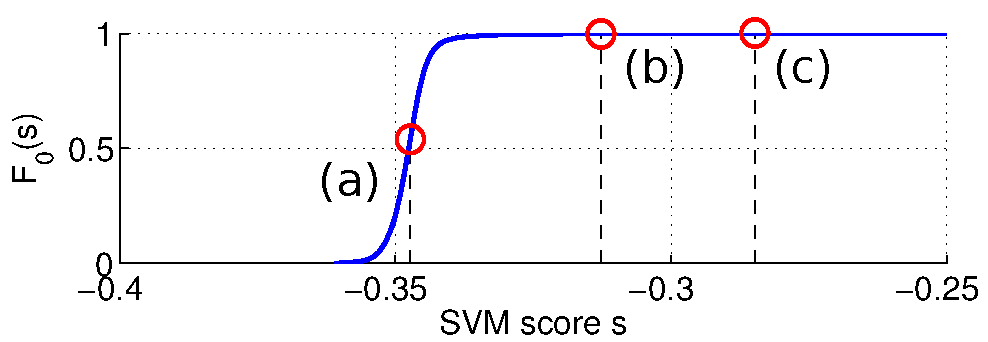
\includegraphics[width=\linewidth]{imgs/wVS3q/2932/graphBigO.pdf}
          \end{minipage} 
          %
          \begin{minipage}{\wii}
            \centering
            \centerline{\scriptsize Target database image $j$}
            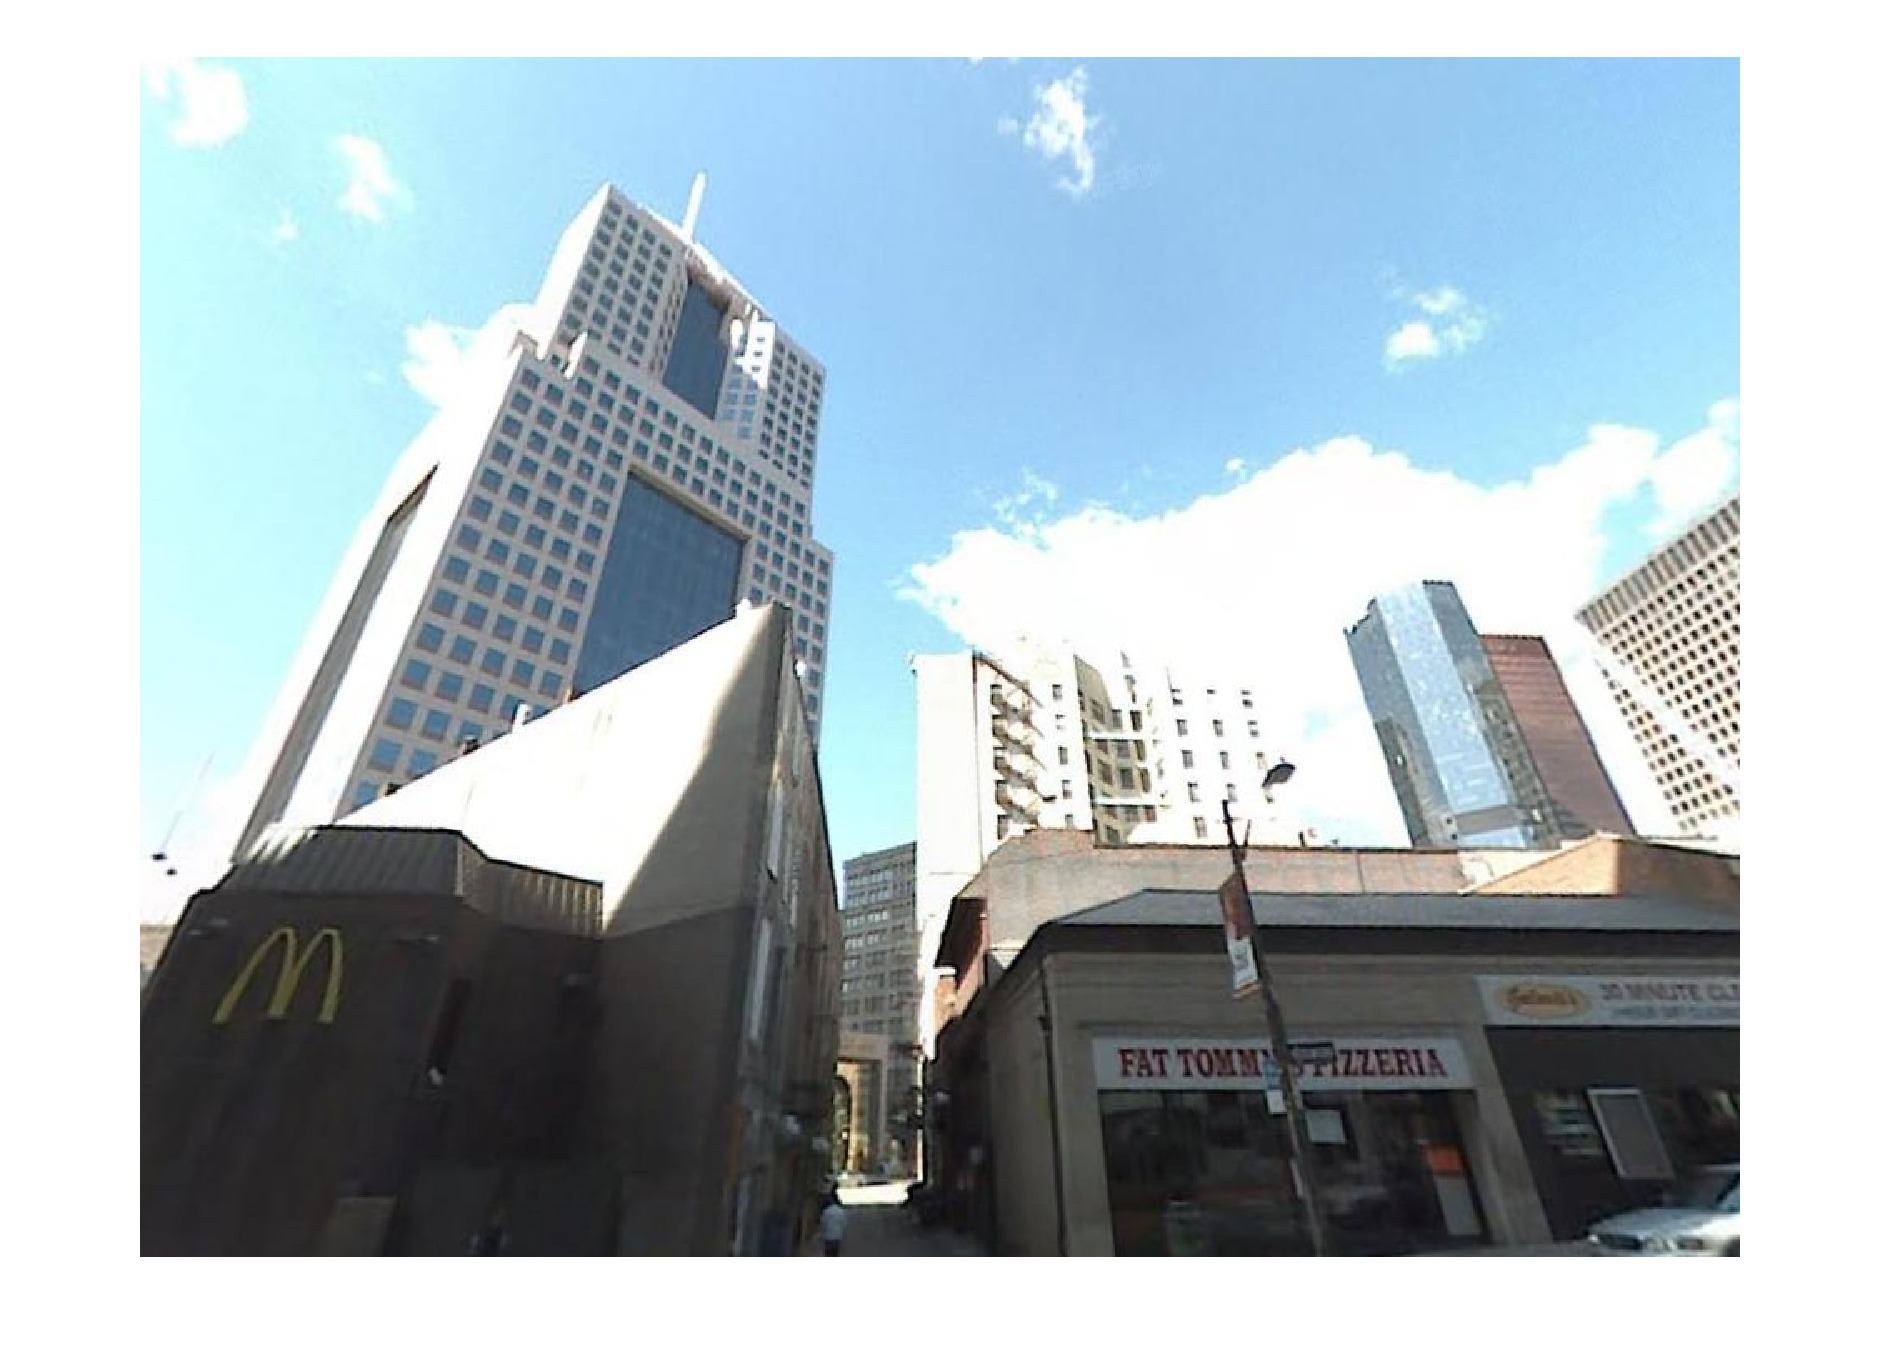
\includegraphics[width=\linewidth]{imgs/wVS3q/2932/j.jpg}
          \end{minipage}  
          \vspace{3mm}
          \\
          \centerline{\scriptsize Classified query images $f_j(q)$} 
          \\
          \begin{minipage}{\wii}
            \centering
            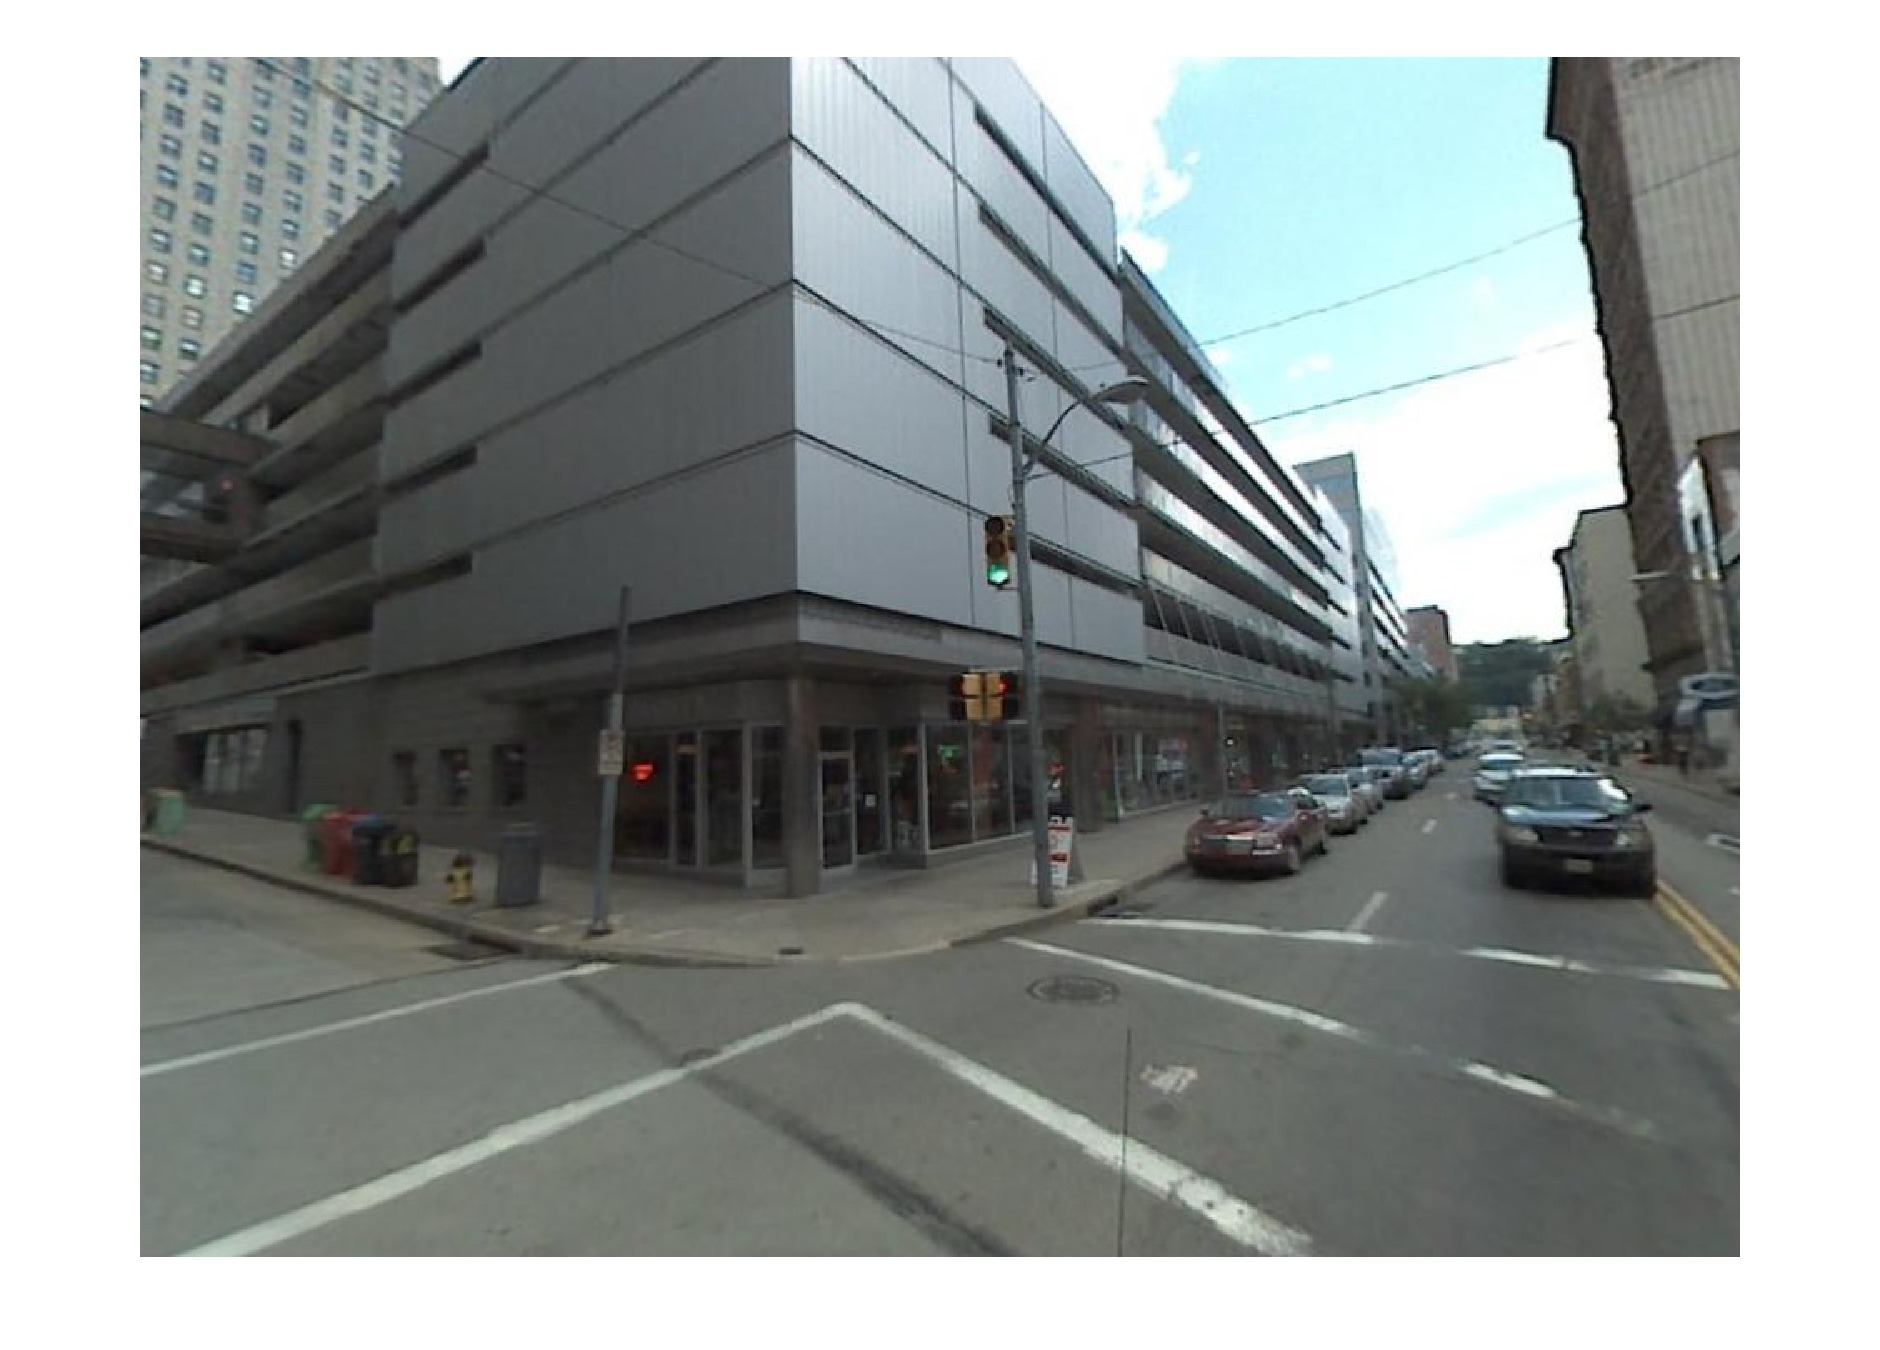
\includegraphics[width=\linewidth]{imgs/wVS3q/2932/a.jpg}
          \end{minipage}  
          \begin{minipage}{\wii}
            \centering
            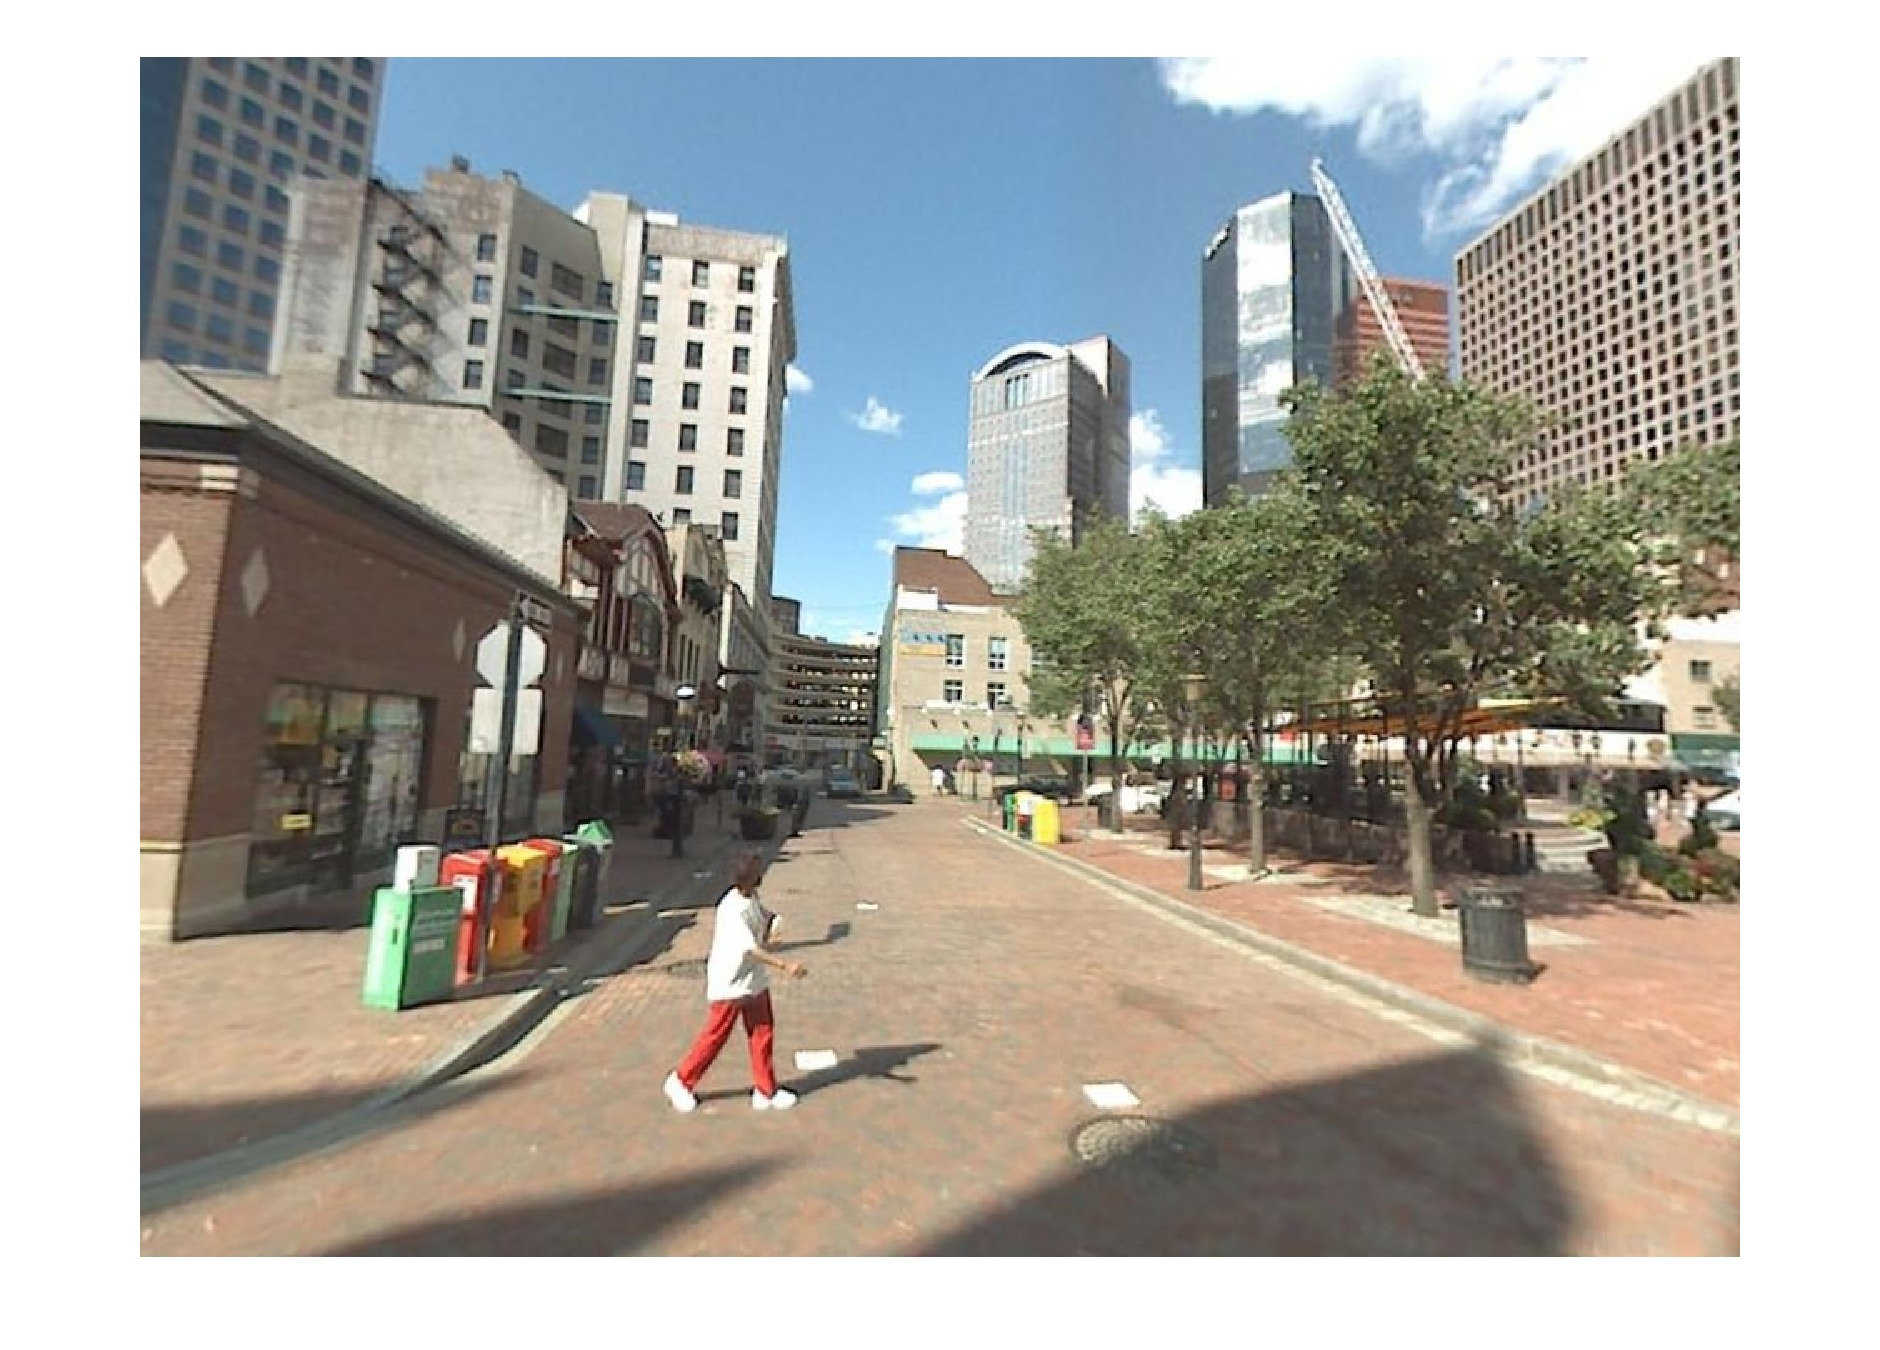
\includegraphics[width=\linewidth]{imgs/wVS3q/2932/b.jpg}
          \end{minipage}  
          \begin{minipage}{\wii}
            \centering
            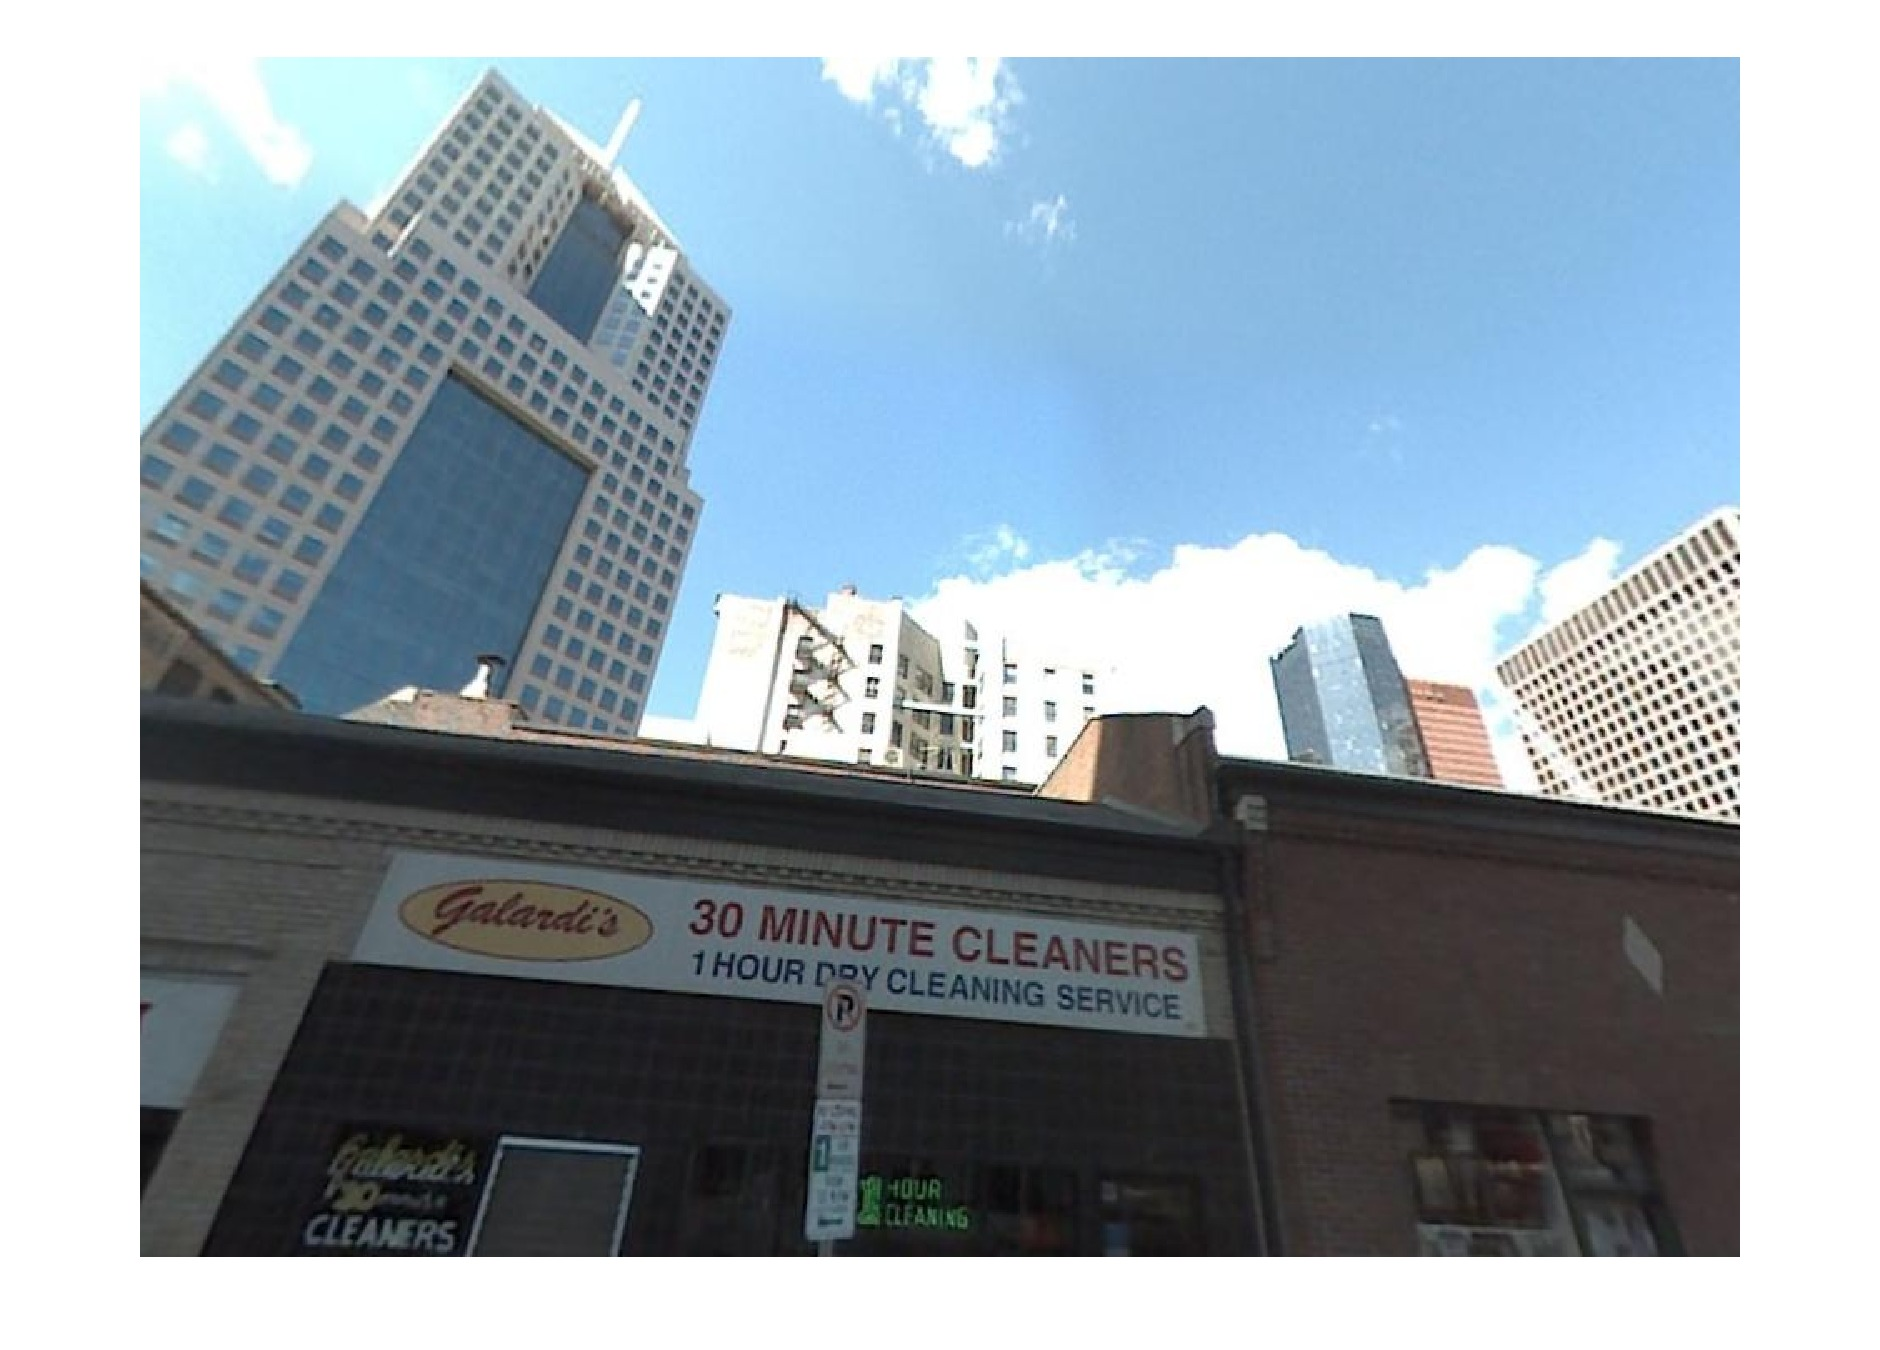
\includegraphics[width=\linewidth]{imgs/wVS3q/2932/c.jpg}
          \end{minipage} 
          \\
          \begin{minipage}{\wii}
            \centering
            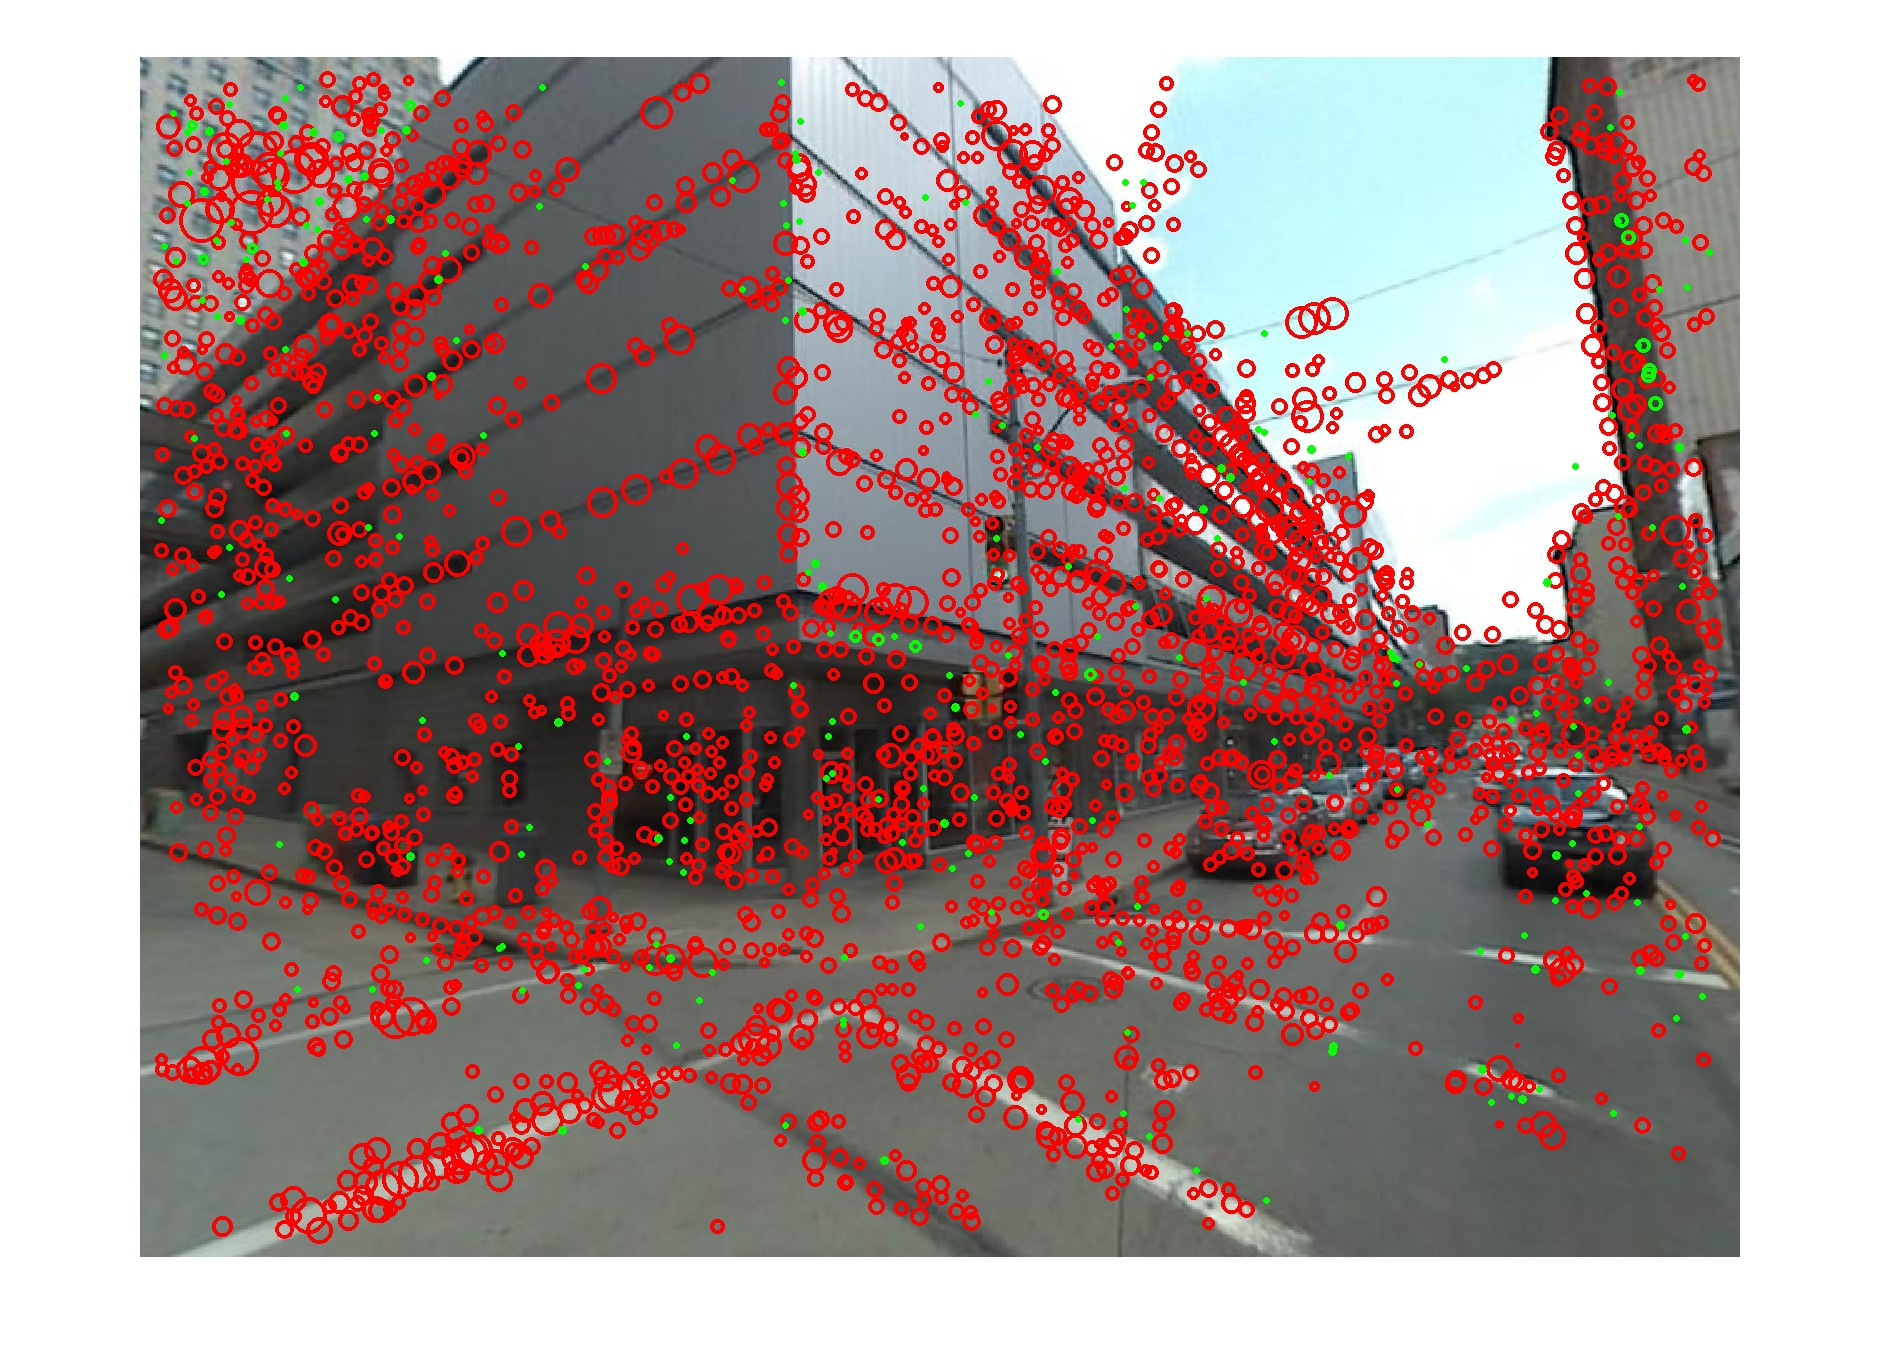
\includegraphics[width=\linewidth]{imgs/wVS3q/2932/aftrs.jpg}
            \newline
            (a)
          \end{minipage}  
          \begin{minipage}{\wii}
            \centering
            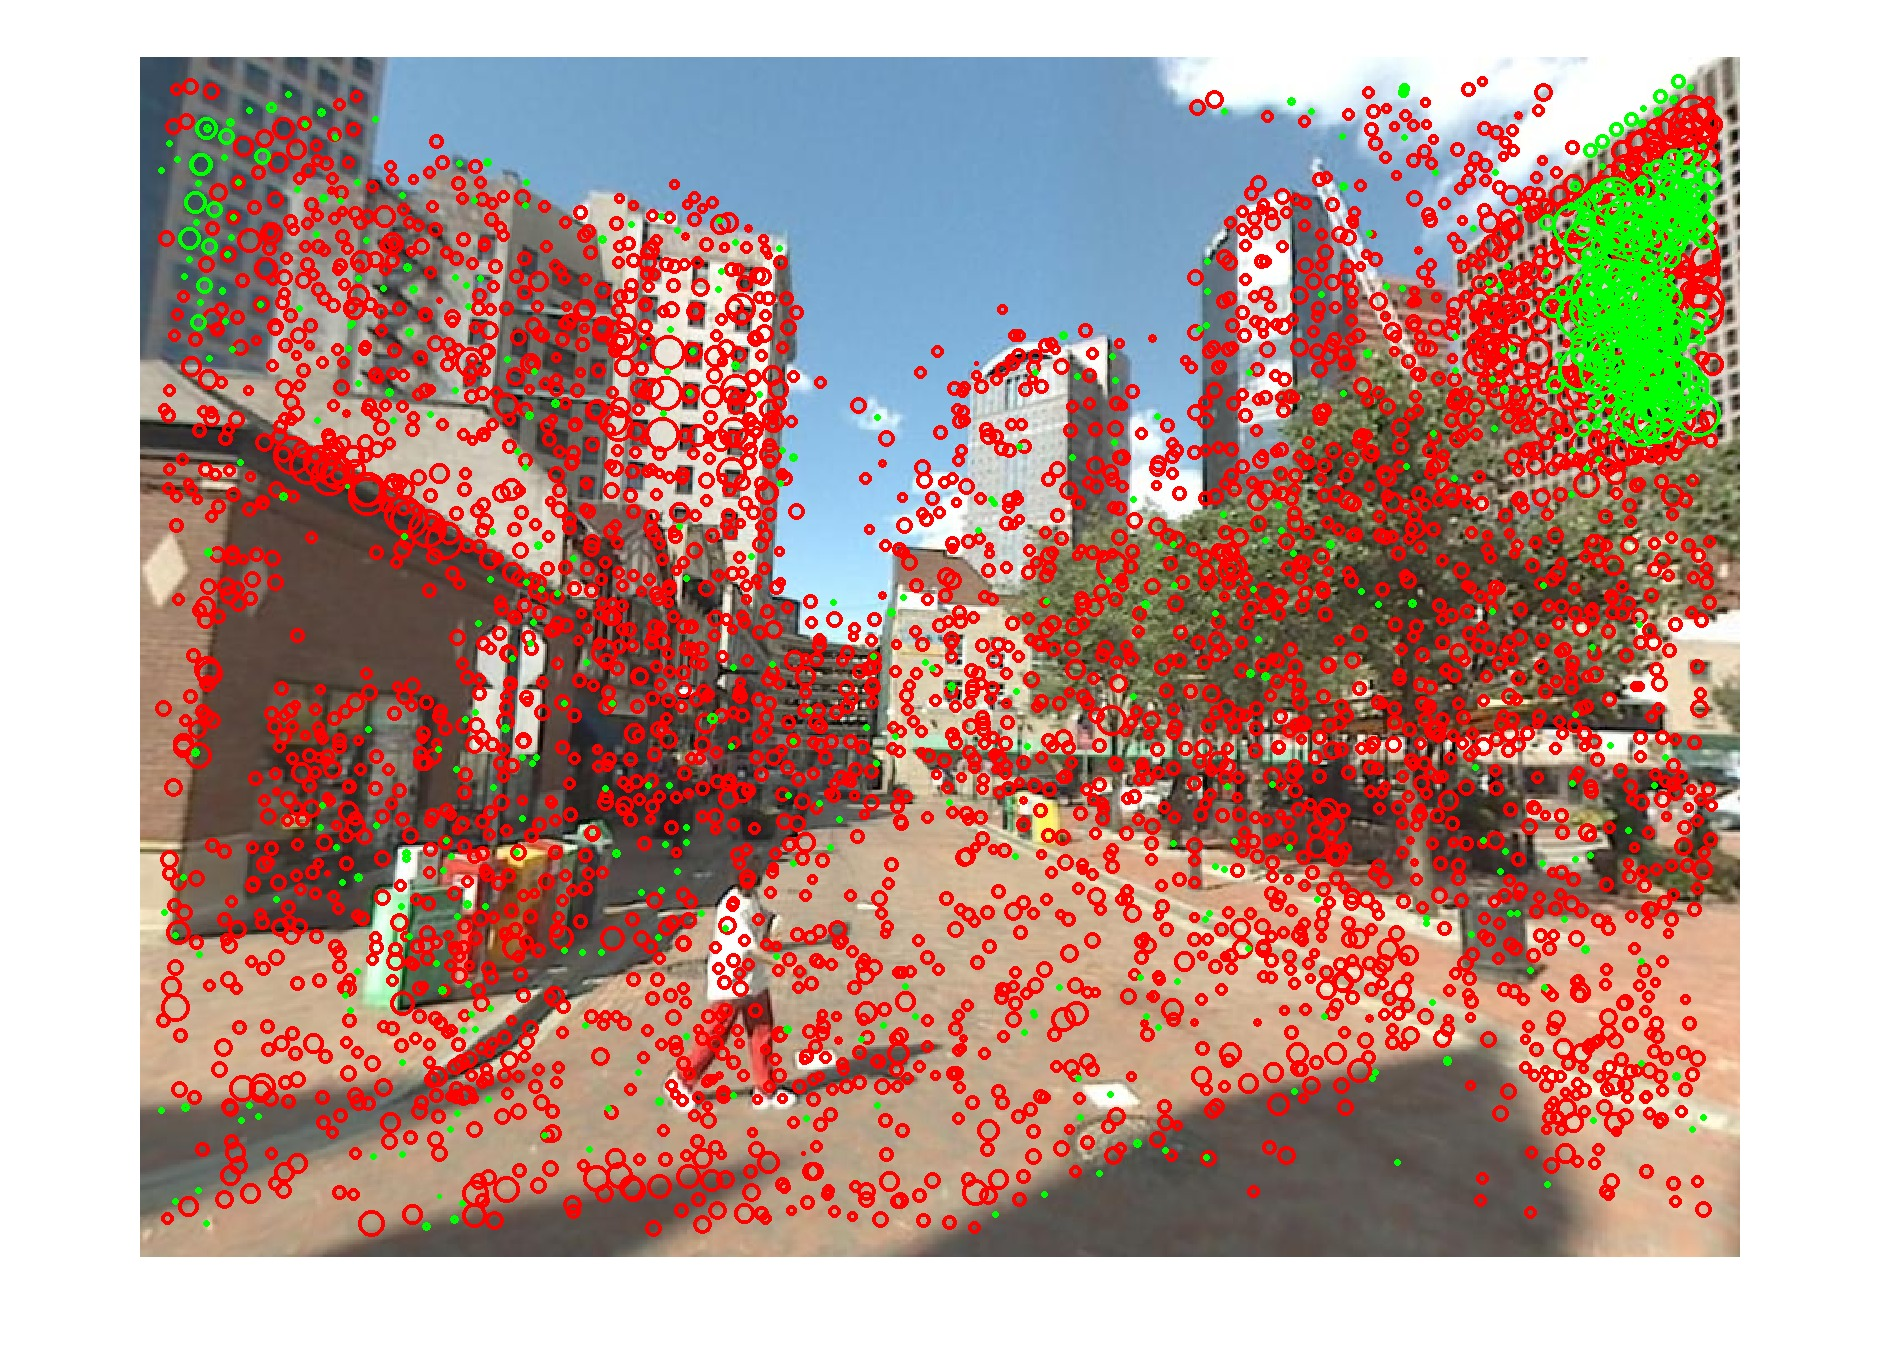
\includegraphics[width=\linewidth]{imgs/wVS3q/2932/bftrs.jpg}
            \newline
            (b)
          \end{minipage}  
          \begin{minipage}{\wii}
            \centering
            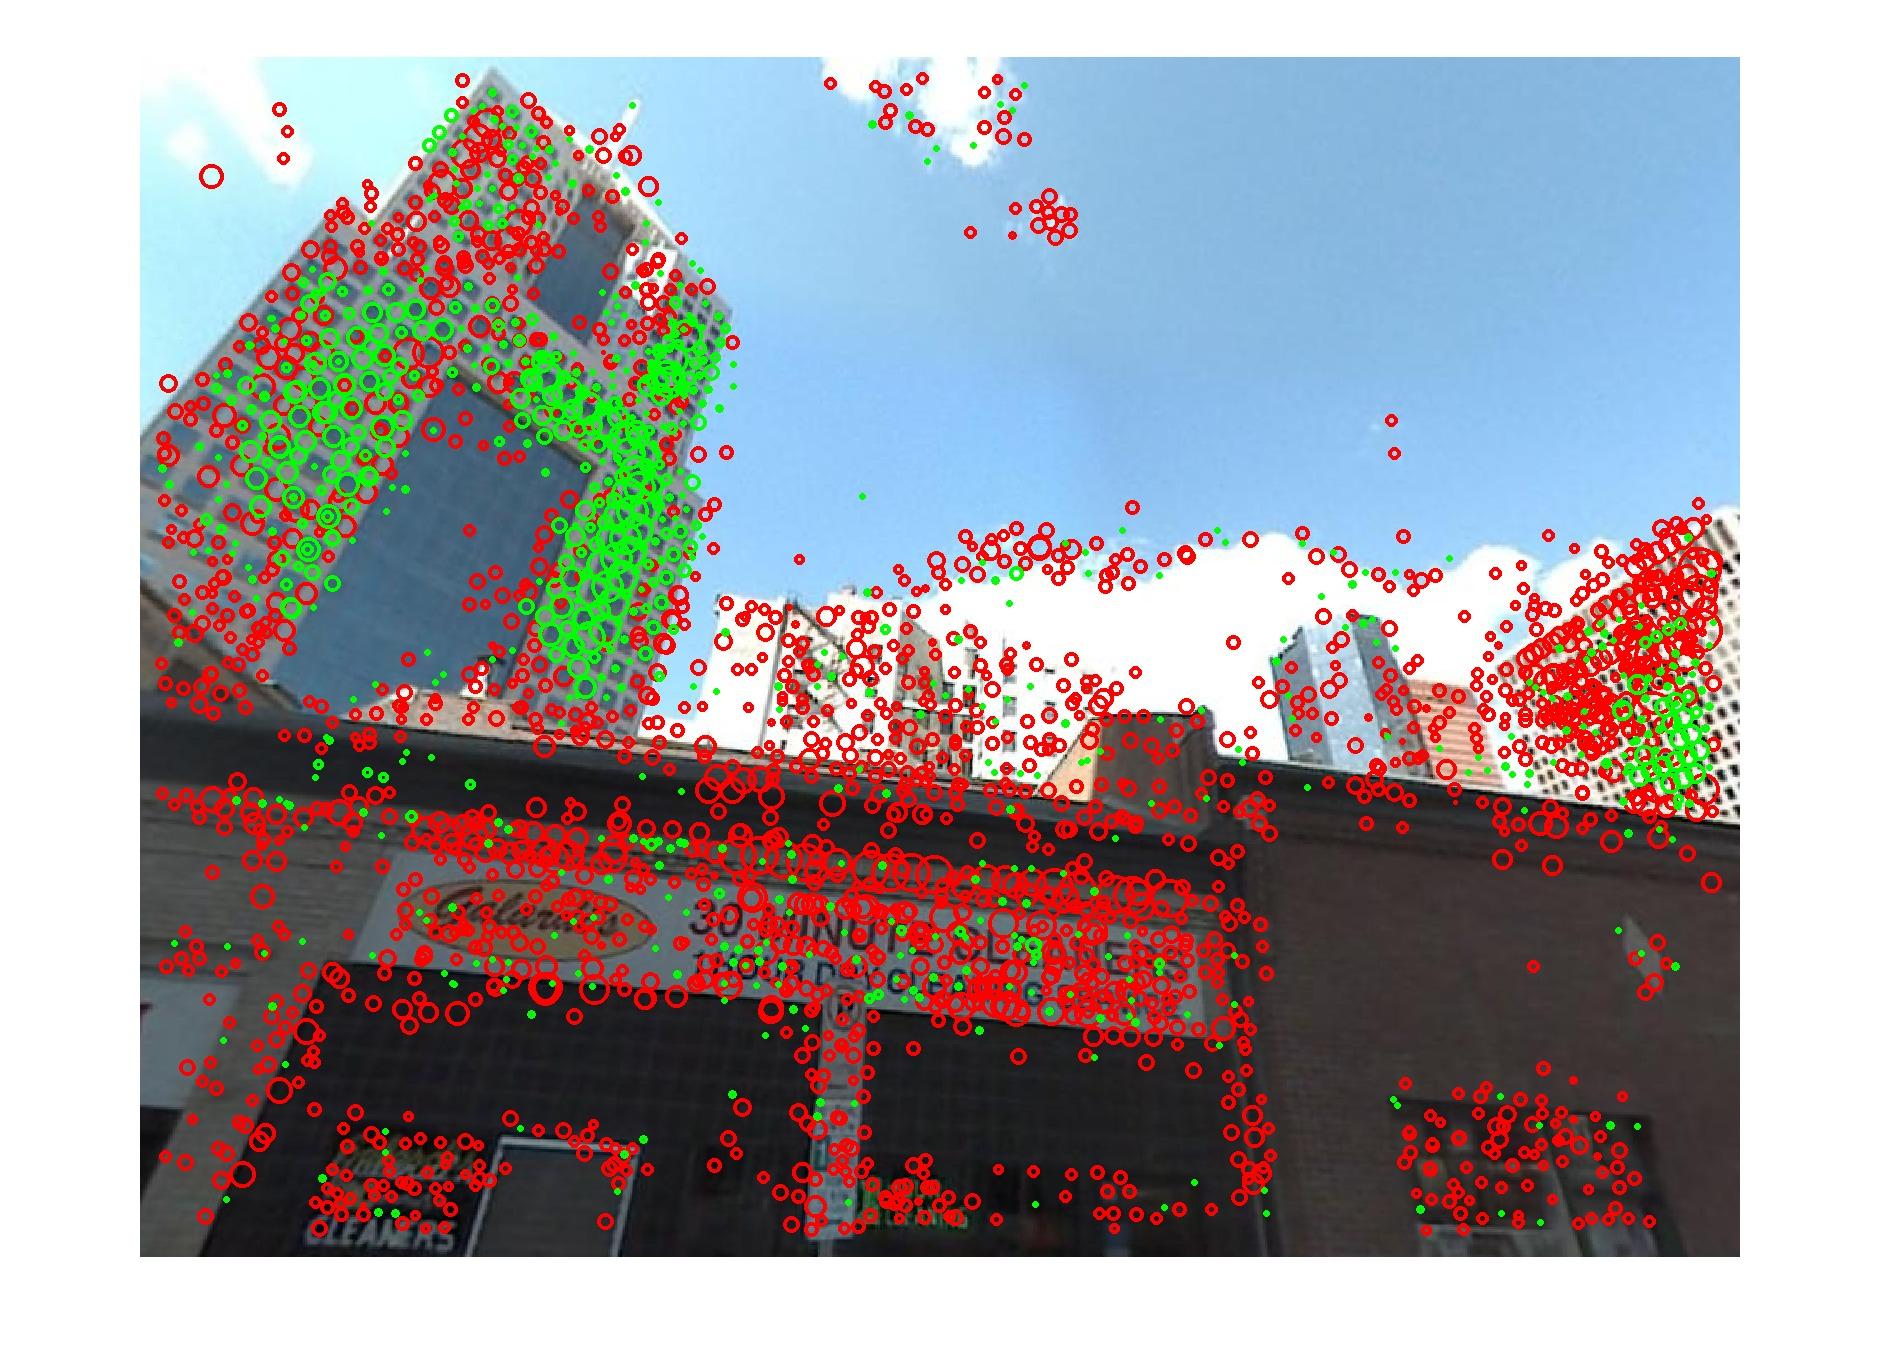
\includegraphics[width=\linewidth]{imgs/wVS3q/2932/cftrs.jpg}
            \newline
            (c)
          \end{minipage} 
    \end{minipage}% right figure
    %
    \vspace*{-2mm}
    \caption{\myCap}
    \label{fig:3qVSw}
        \vspace*{2mm}
    \end{figure*}
    \vspace*{-2mm}
    \caption{
          {\bf  A visualization of learnt feature weights for two database images. In each panel:} 
         \emph{first~row:} (Right) Target database image $j$. (Left) Cumulative density function (or calibrated score) learnt for the SVM scores of the corresponding classifier $f_j$ \textcolor{petr}{(notice that $cdf$s are not identical)};  three query images displayed on the \emph{second row} are represented by their SVM scores and cdf values $F_0(s)$, denoted (a)-(c) on the graph. \emph{Third~row:} A visualization of the contribution of each feature to the SVM score for the corresponding query image. Red circles represent features with negative weights while green circles correspond to features with positive weights. The area of each circle is proportional to the contribution of the corresponding feature to the SVM score.
         %
         Notice that the correctly localized queries (c) contain more green colored features than queries from other places (b) and (a).
         {\it Left panel:} Query (b) gets a high score because the building has orange and white stripes similar to the the sun-blinds of the bakery, which are features that also have large positive weights in the query image (c) of the correct place.
         {\it Right panel:} Query (b) is in fact also an image of the same location with a portion of the left skyscraper in the target image detected in the upper left corner and the side of the rightmost building in the target image detected in the top right corner. Both are clearly detected by the method as indicated by a large quantity of green circles in the corresponding regions.
    }
    \label{fig:3qVSw}
    \vspace*{2mm}
  \end{figure*}


    %%% FIGURE: Visualization, examples for BOW p-val
    \begin{figure*}[t!]
              %%%%%%%%%%% Example 1 %%%%%%%%%%%%%%%
        \begin{minipage}{1.0\linewidth}
        \end{minipage}
        % QUERY image
        \begin{minipage}{0.34\linewidth}
            \centering
            \vspace{0mm}
            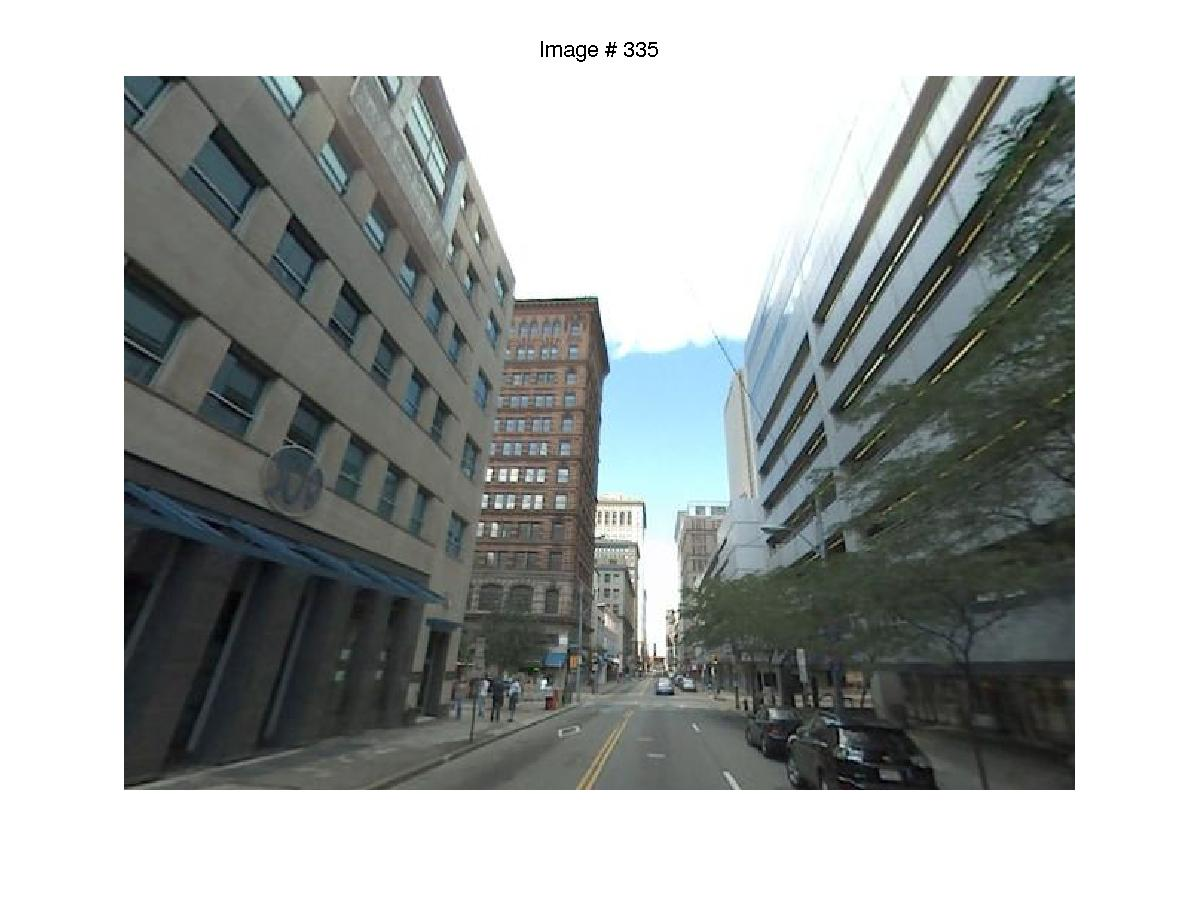
\includegraphics[trim = 45mm 40mm 45mm 30mm, clip=true,height=36mm]{imgs/Pval/exImproved02/query.jpg}
        \end{minipage}
        % Retrieved images
        \begin{minipage}{0.75\linewidth}
            % FV e-SVM
            \begin{minipage}{\linewidth} 
                \colorbox{myGreen}{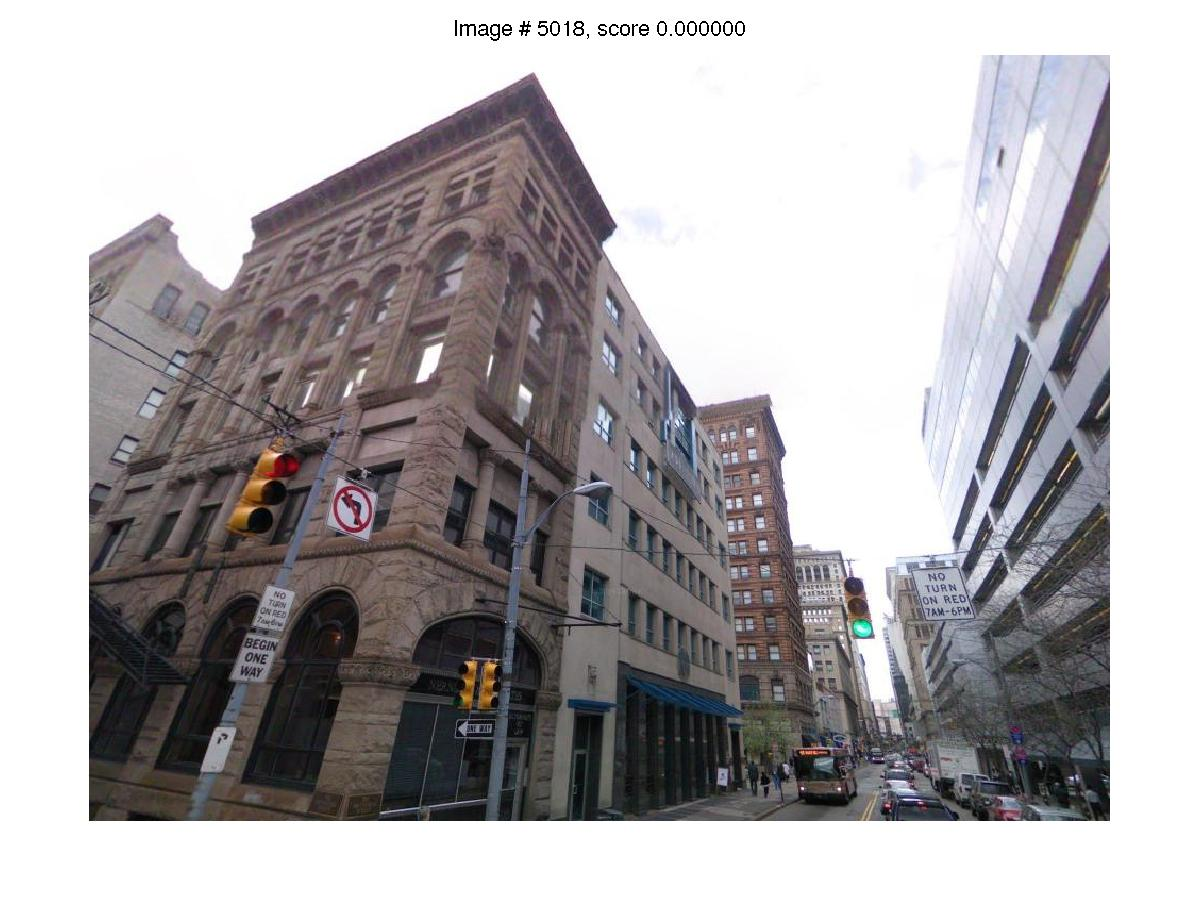
\includegraphics[trim = 35mm 30mm 35mm 30mm, clip=true, height=16mm]{imgs/Pval/exImproved02/improvedPval01.jpg}}
                \colorbox{myGreen}{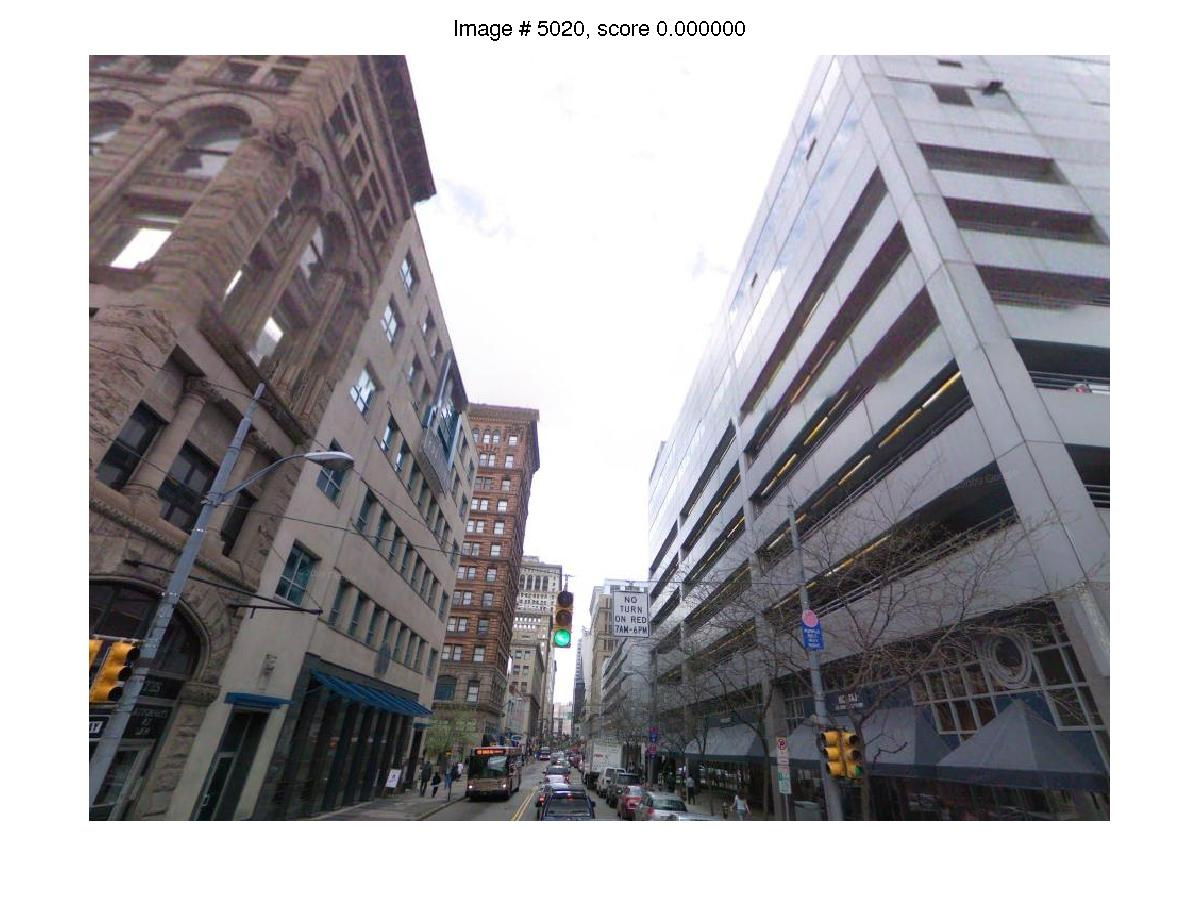
\includegraphics[trim = 35mm 30mm 35mm 30mm, clip=true, height=16mm]{imgs/Pval/exImproved02/improvedPval02.jpg}}
                \colorbox{myGreen}{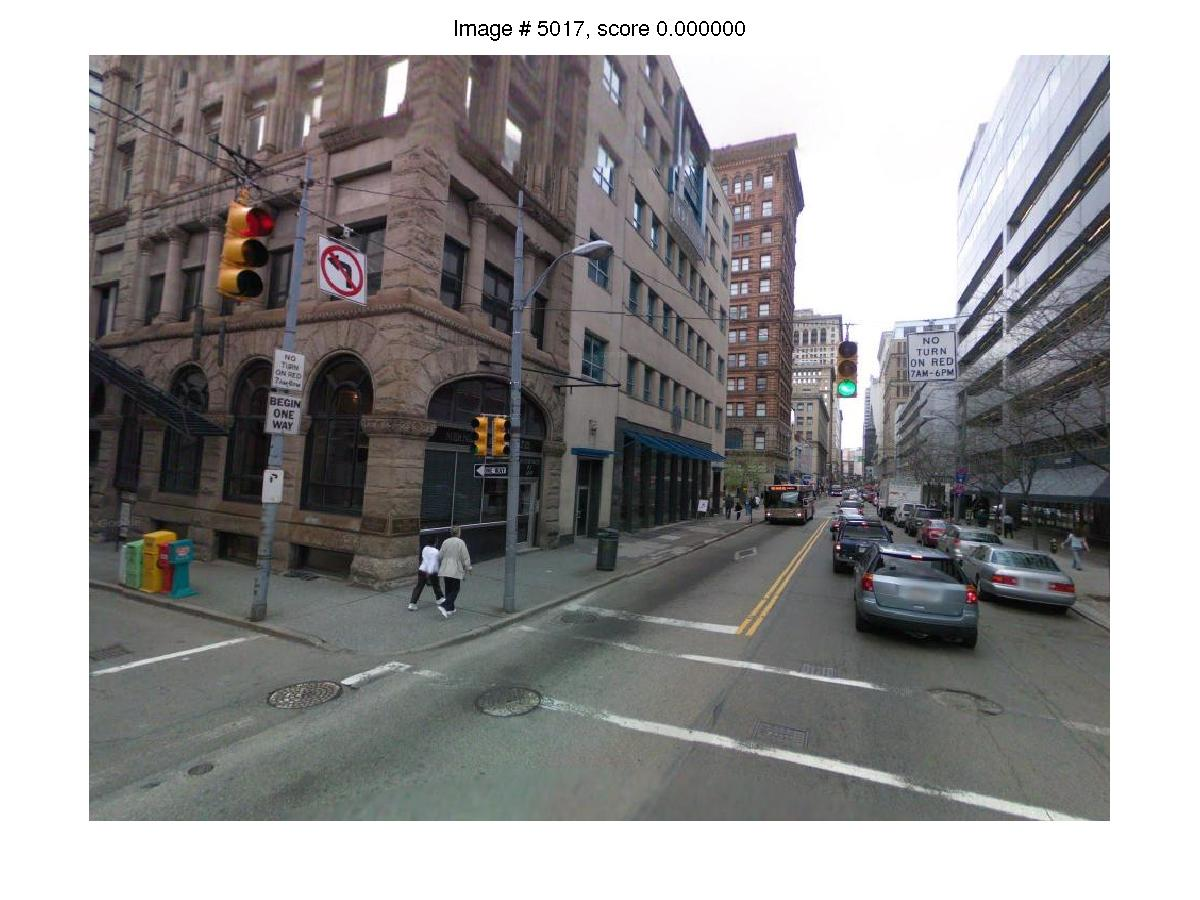
\includegraphics[trim = 35mm 30mm 35mm 30mm, clip=true, height=16mm]{imgs/Pval/exImproved02/improvedPval03.jpg}}
                \colorbox{myGreen}{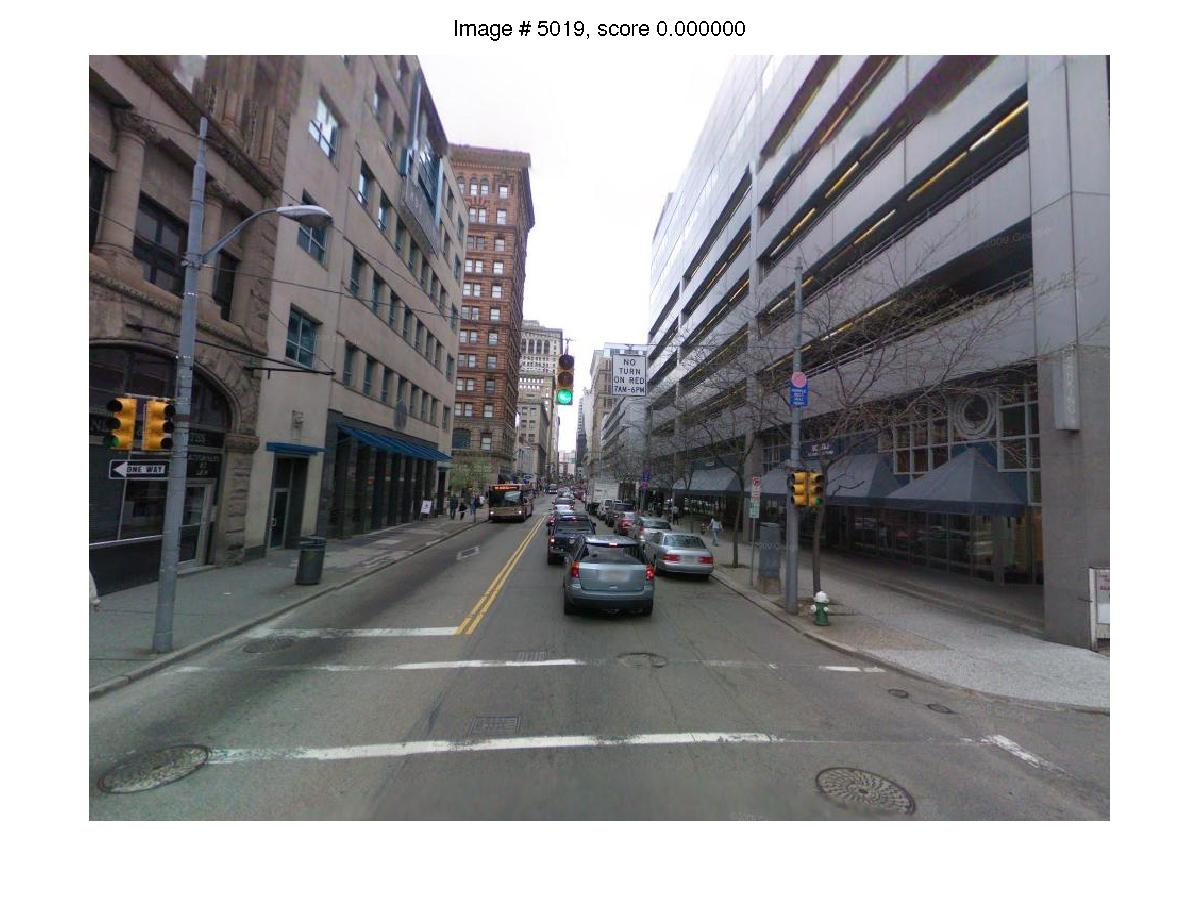
\includegraphics[trim = 35mm 30mm 35mm 30mm, clip=true, height=16mm]{imgs/Pval/exImproved02/improvedPval04.jpg}}
            \end{minipage}
            \\
            \begin{minipage}{\linewidth}
                \colorbox{myRed}{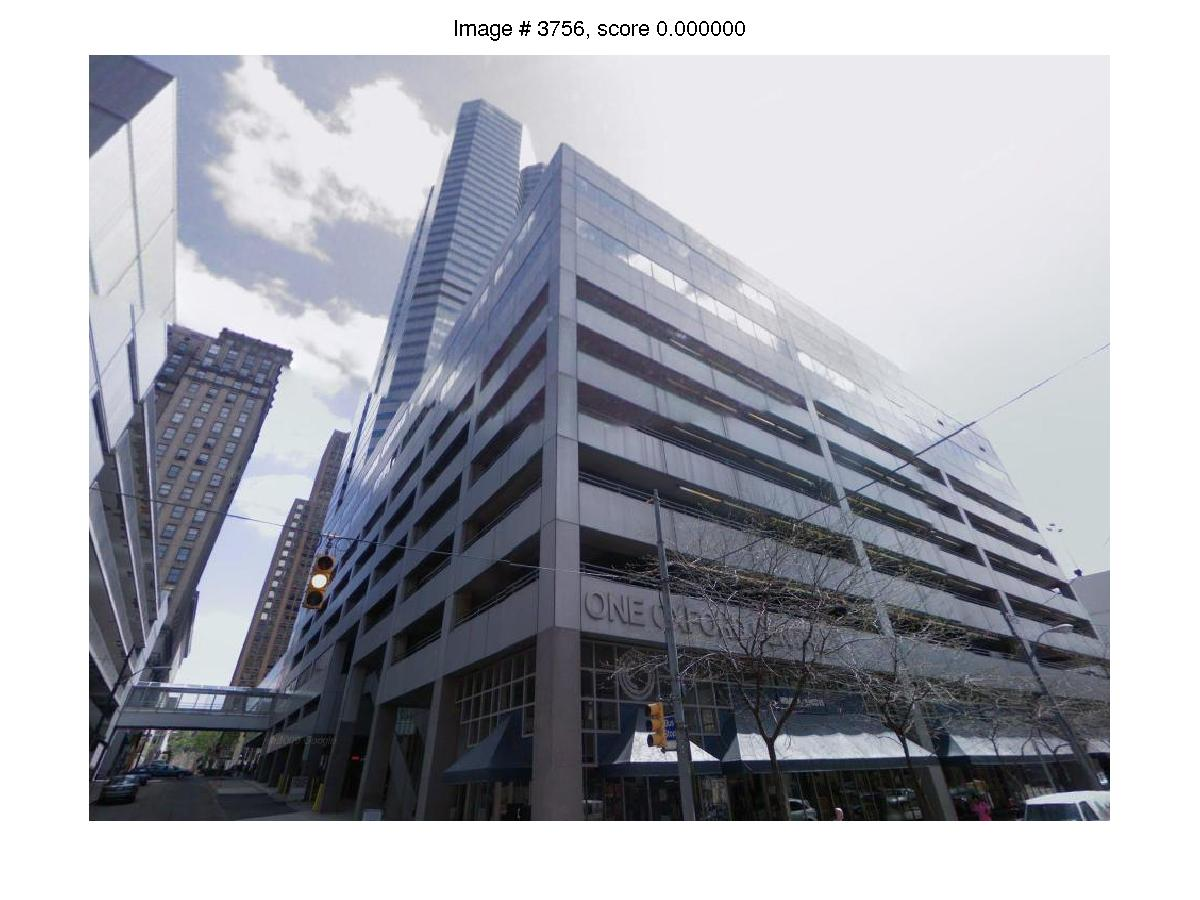
\includegraphics[trim = 35mm 30mm 35mm 30mm, clip=true, height=16mm]{imgs/Pval/exImproved02/improved01.jpg}}
                \colorbox{myRed}{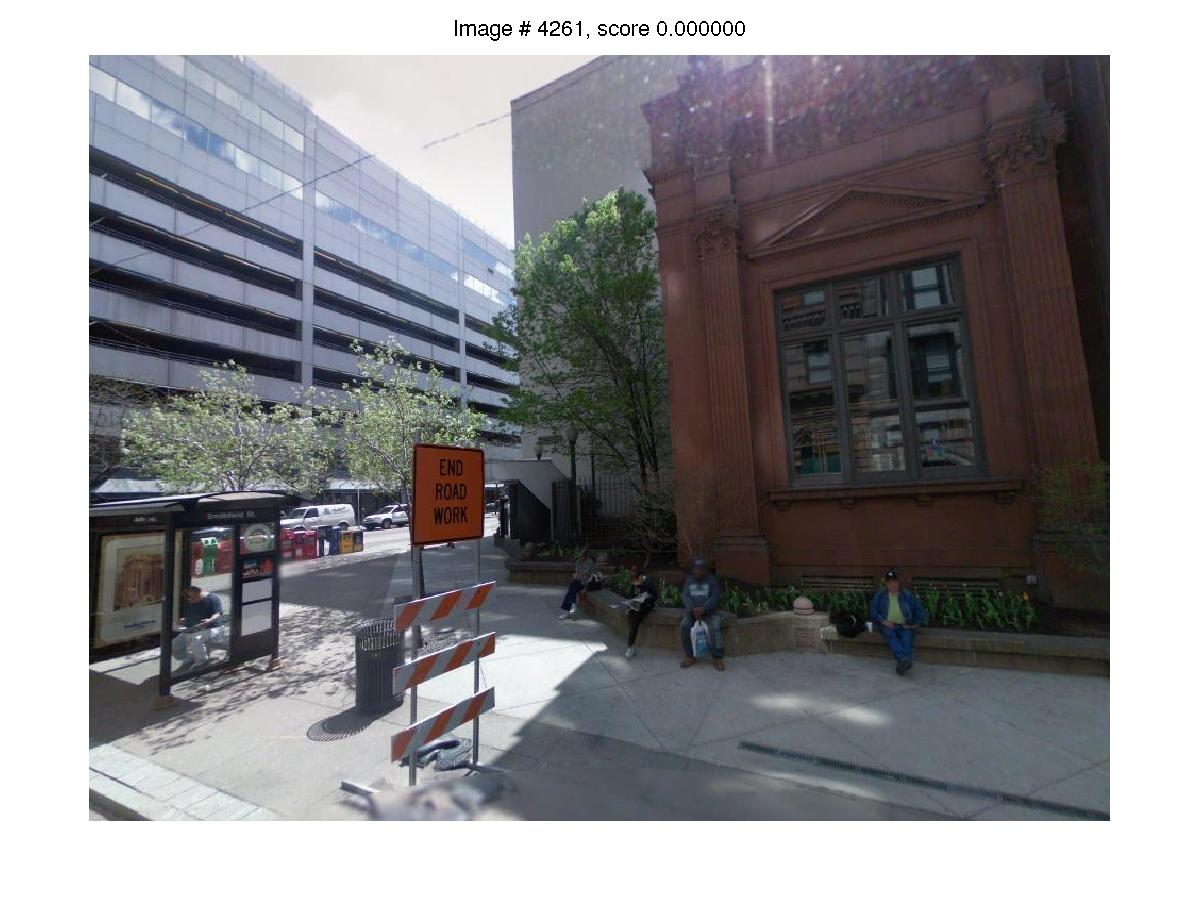
\includegraphics[trim = 35mm 30mm 35mm 30mm, clip=true, height=16mm]{imgs/Pval/exImproved02/improved02.jpg}}
                \colorbox{myRed}{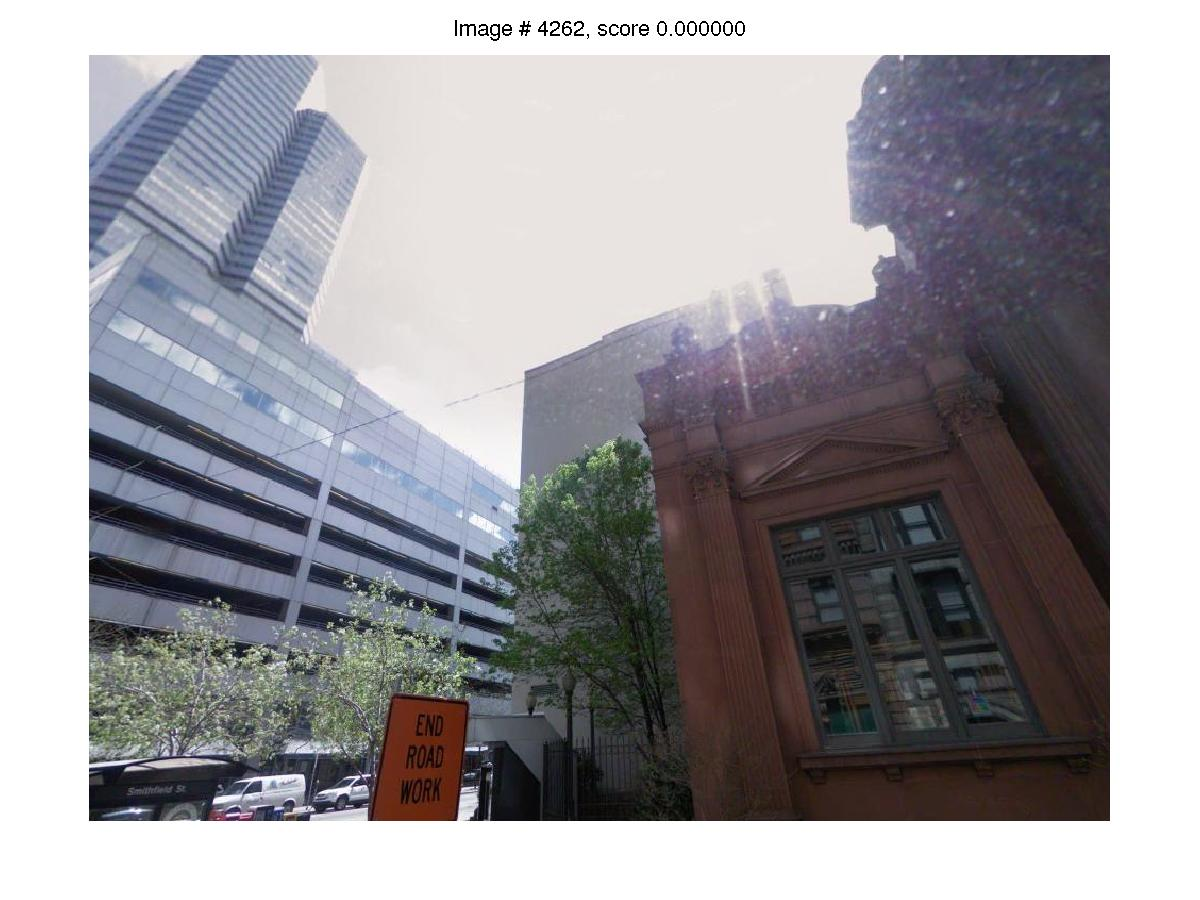
\includegraphics[trim = 35mm 30mm 35mm 30mm, clip=true, height=16mm]{imgs/Pval/exImproved02/improved03.jpg}}
                \colorbox{myRed}{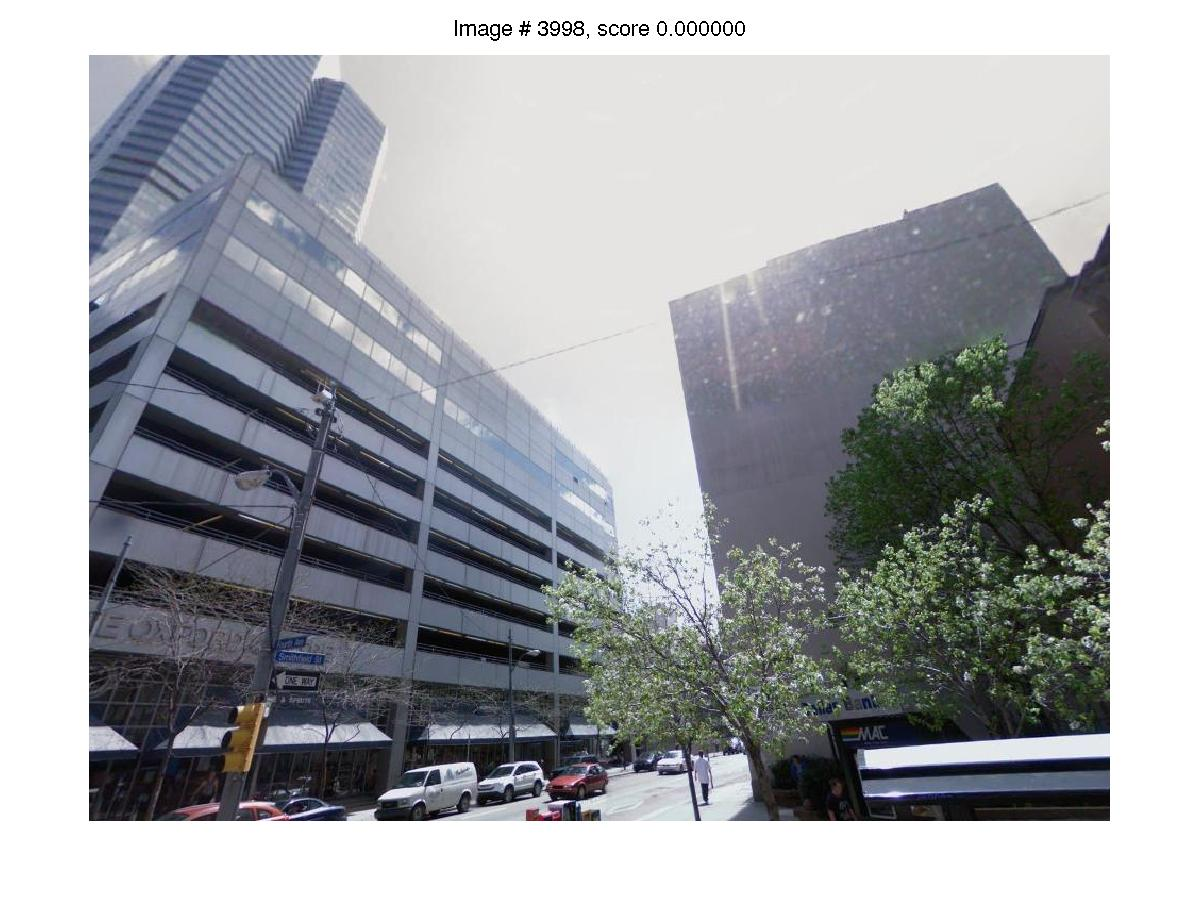
\includegraphics[trim = 35mm 30mm 35mm 30mm, clip=true, height=16mm]{imgs/Pval/exImproved02/improved04.jpg}}
            \end{minipage} 
        \end{minipage}
        \vspace{3mm}
        \\
        % %%%%%%%%%%% Example 2 %%%%%%%%%%%%%%%
        % \begin{minipage}{0.34\linewidth}
        %     \centering
        %     \vspace{0mm}
        %     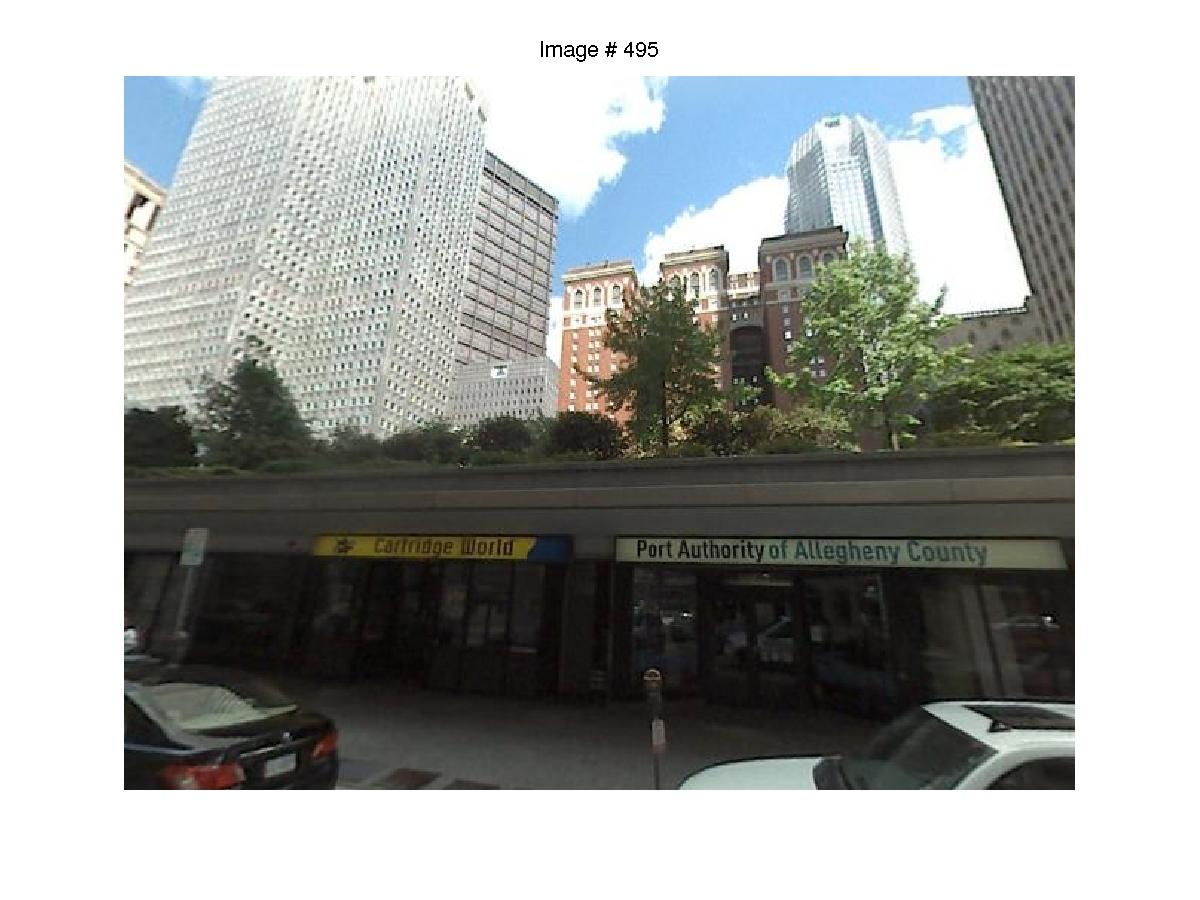
\includegraphics[trim = 45mm 40mm 45mm 30mm, clip=true, height=36mm]{imgs/Pval/exImproved03/query.jpg}
        % \end{minipage}
        % % Retrieved images
        % \begin{minipage}{0.75\linewidth}
        %     % FV e-SVM
        %     \begin{minipage}{\linewidth} 
        %         \colorbox{myGreen}{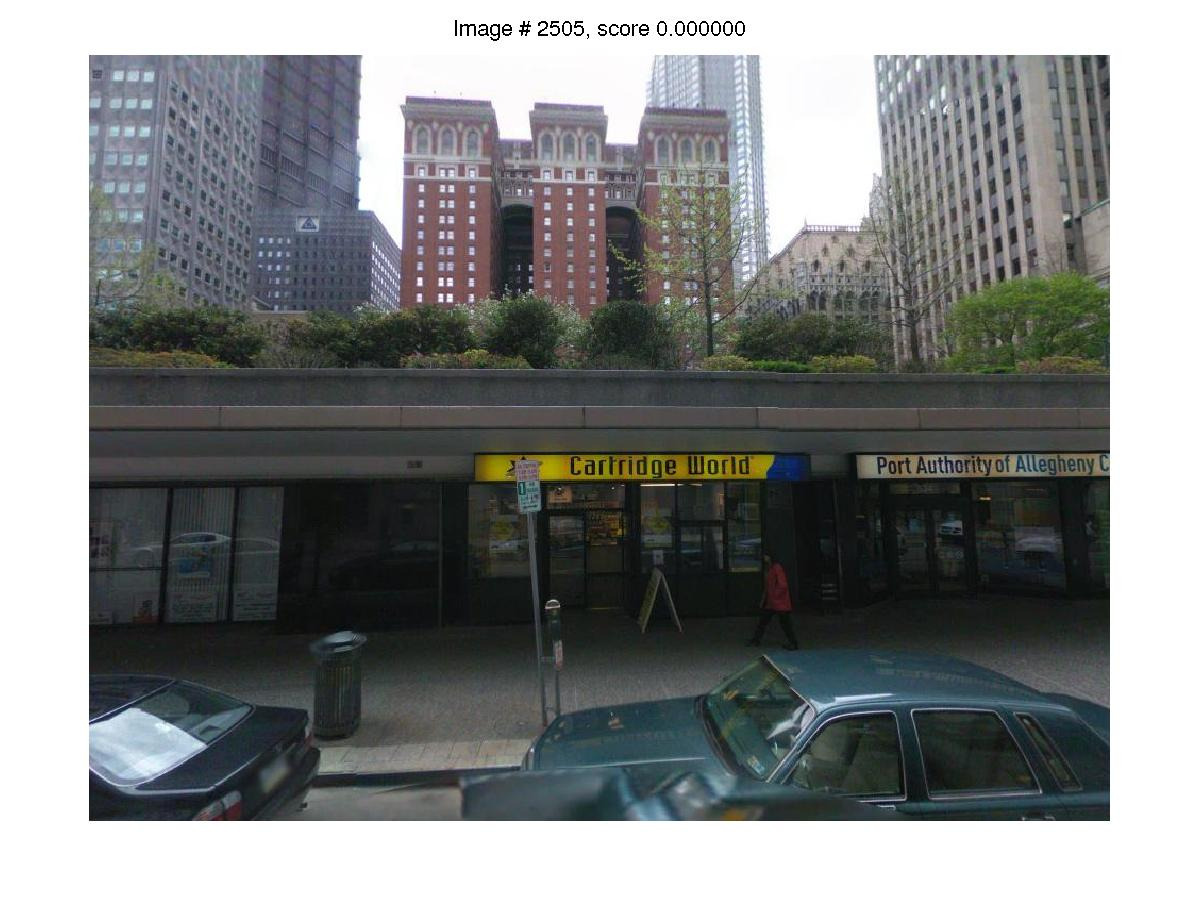
\includegraphics[trim = 35mm 30mm 35mm 30mm, clip=true, height=16mm]{imgs/Pval/exImproved03/improvedPval01.jpg}}
        %         \colorbox{myGreen}{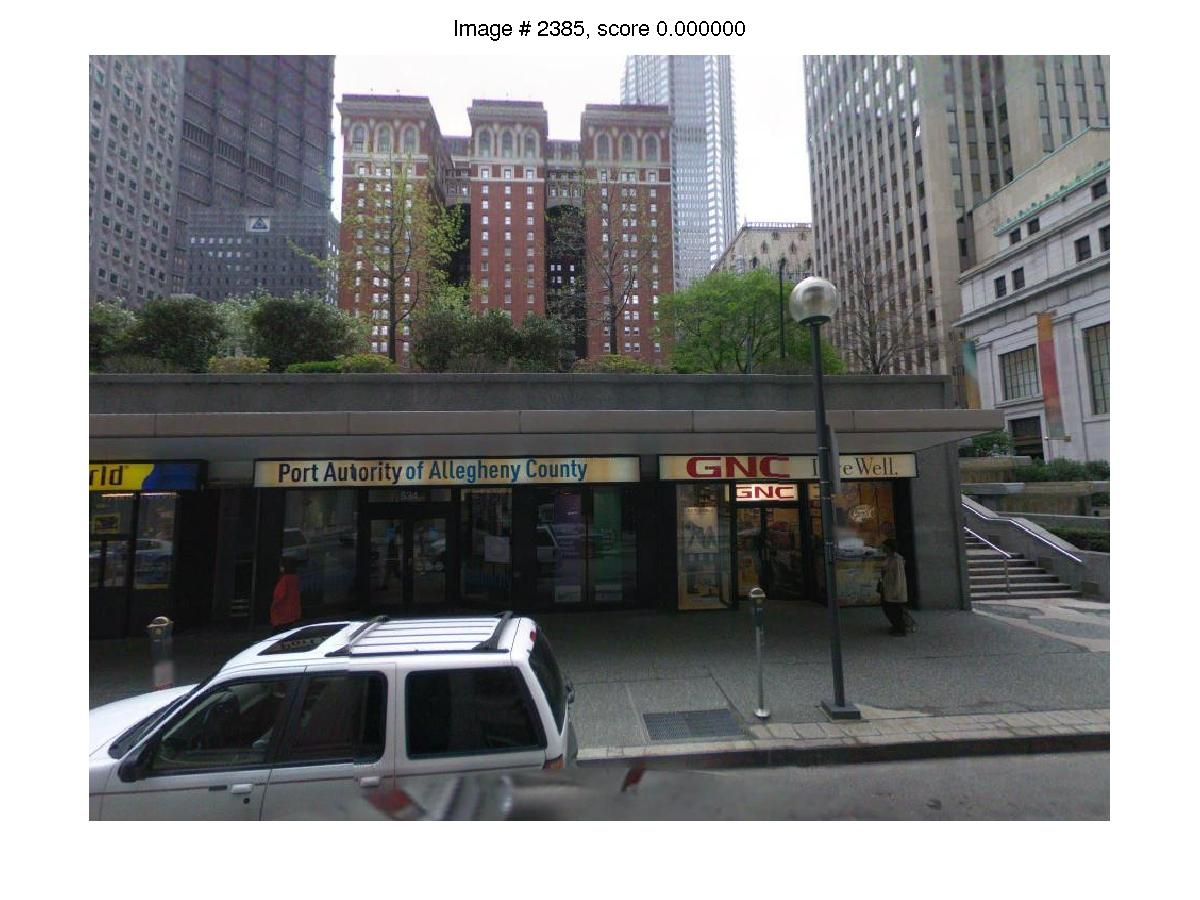
\includegraphics[trim = 35mm 30mm 35mm 30mm, clip=true, height=16mm]{imgs/Pval/exImproved03/improvedPval02.jpg}}
        %         \colorbox{myGreen}{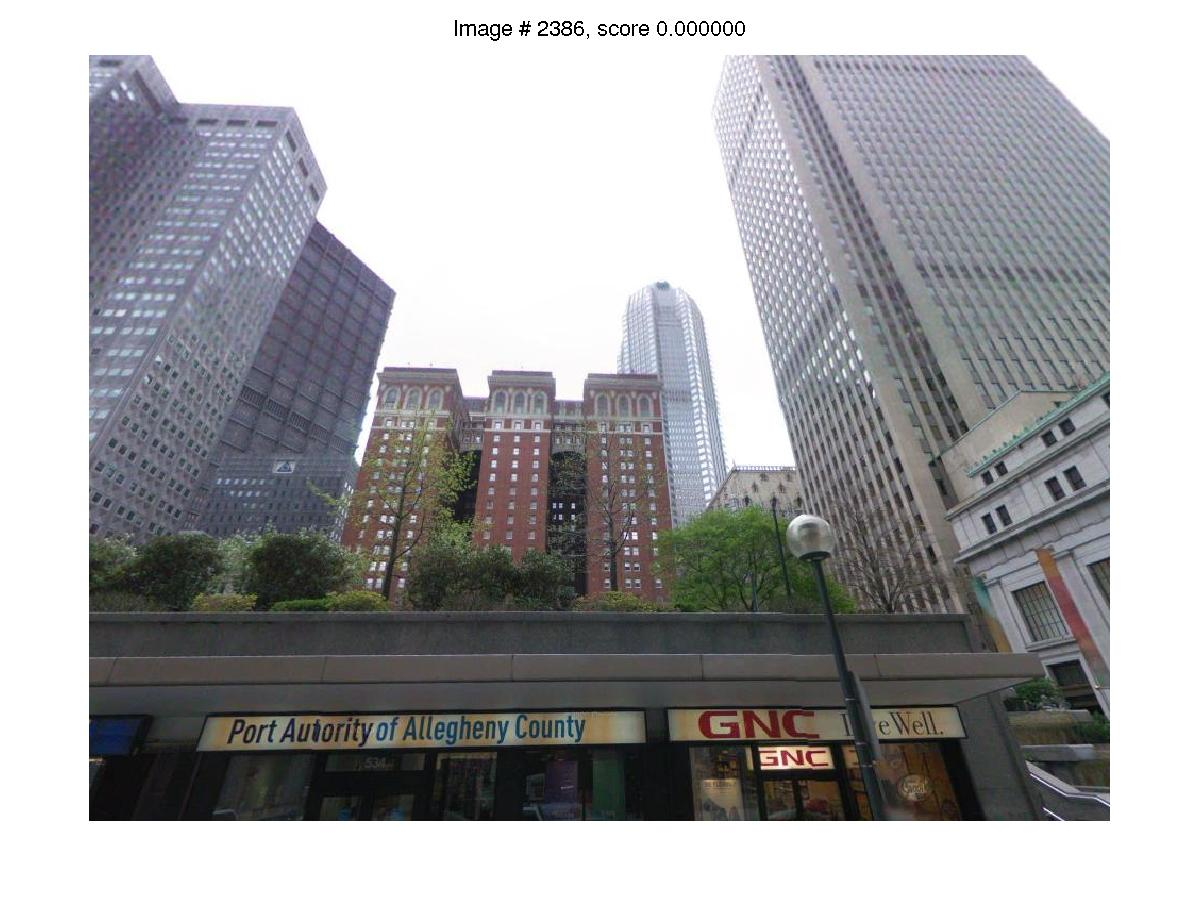
\includegraphics[trim = 35mm 30mm 35mm 30mm, clip=true, height=16mm]{imgs/Pval/exImproved03/improvedPval03.jpg}}
        %         \colorbox{myGreen}{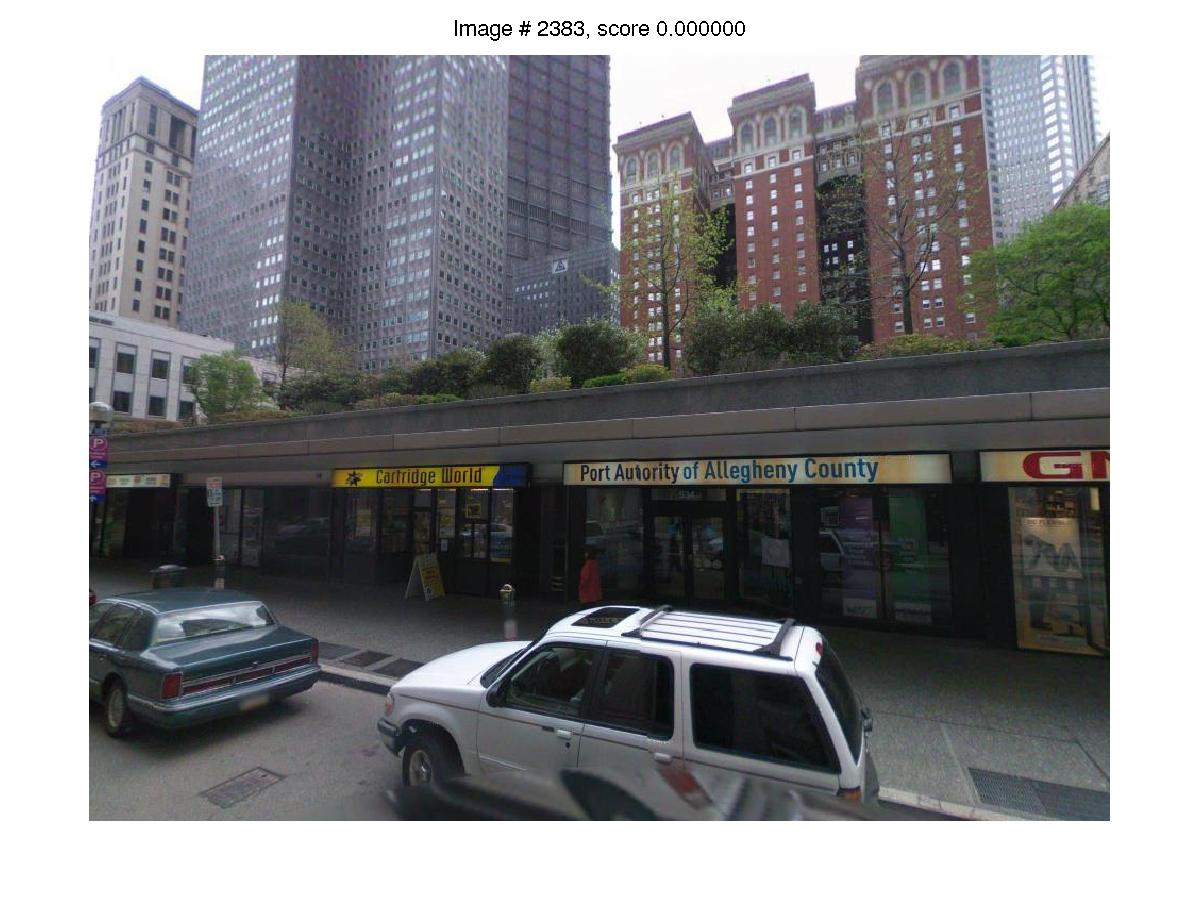
\includegraphics[trim = 35mm 30mm 35mm 30mm, clip=true, height=16mm]{imgs/Pval/exImproved03/improvedPval04.jpg}}
        %     \end{minipage}
        %     \\
        %     \begin{minipage}{\linewidth}
        %         \colorbox{myRed}{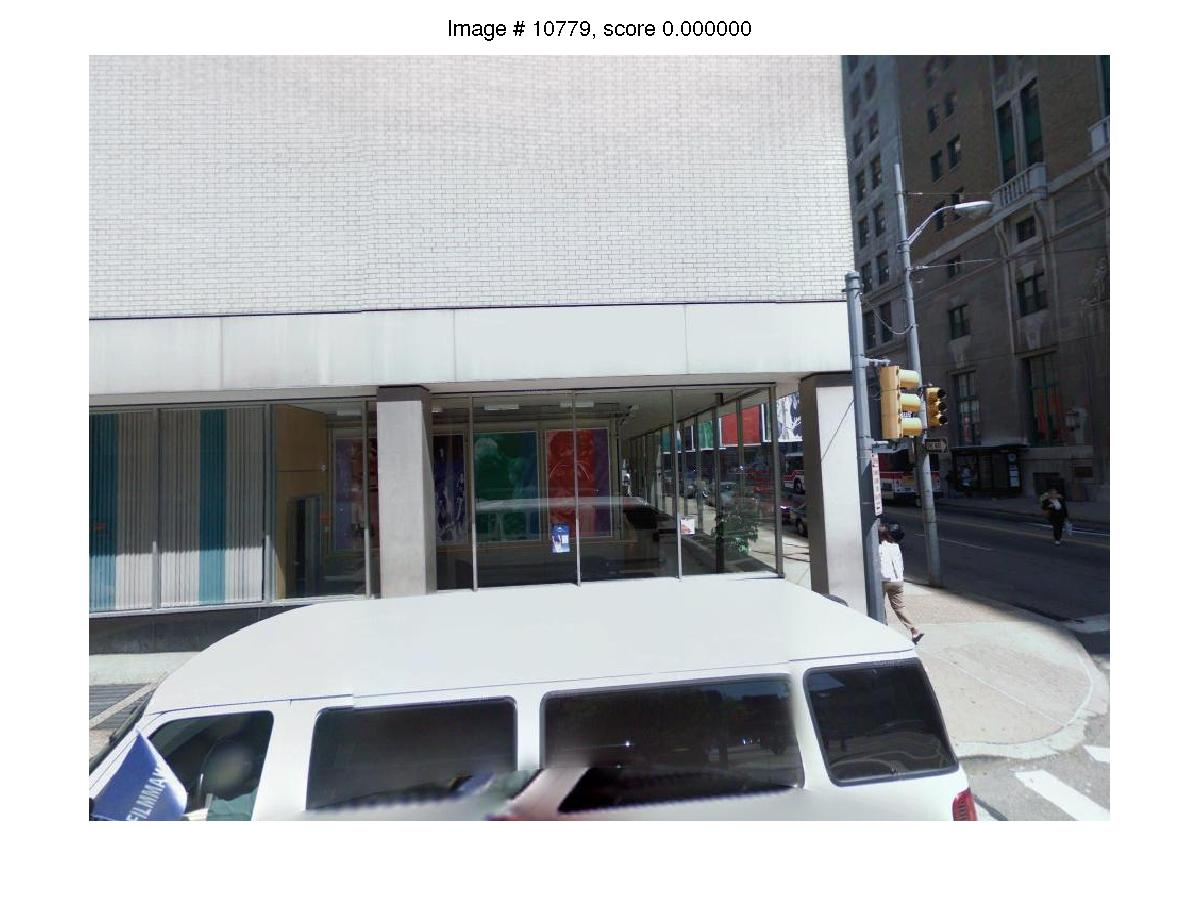
\includegraphics[trim = 35mm 30mm 35mm 30mm, clip=true, height=16mm]{imgs/Pval/exImproved03/improved01.jpg}}
        %         \colorbox{myRed}{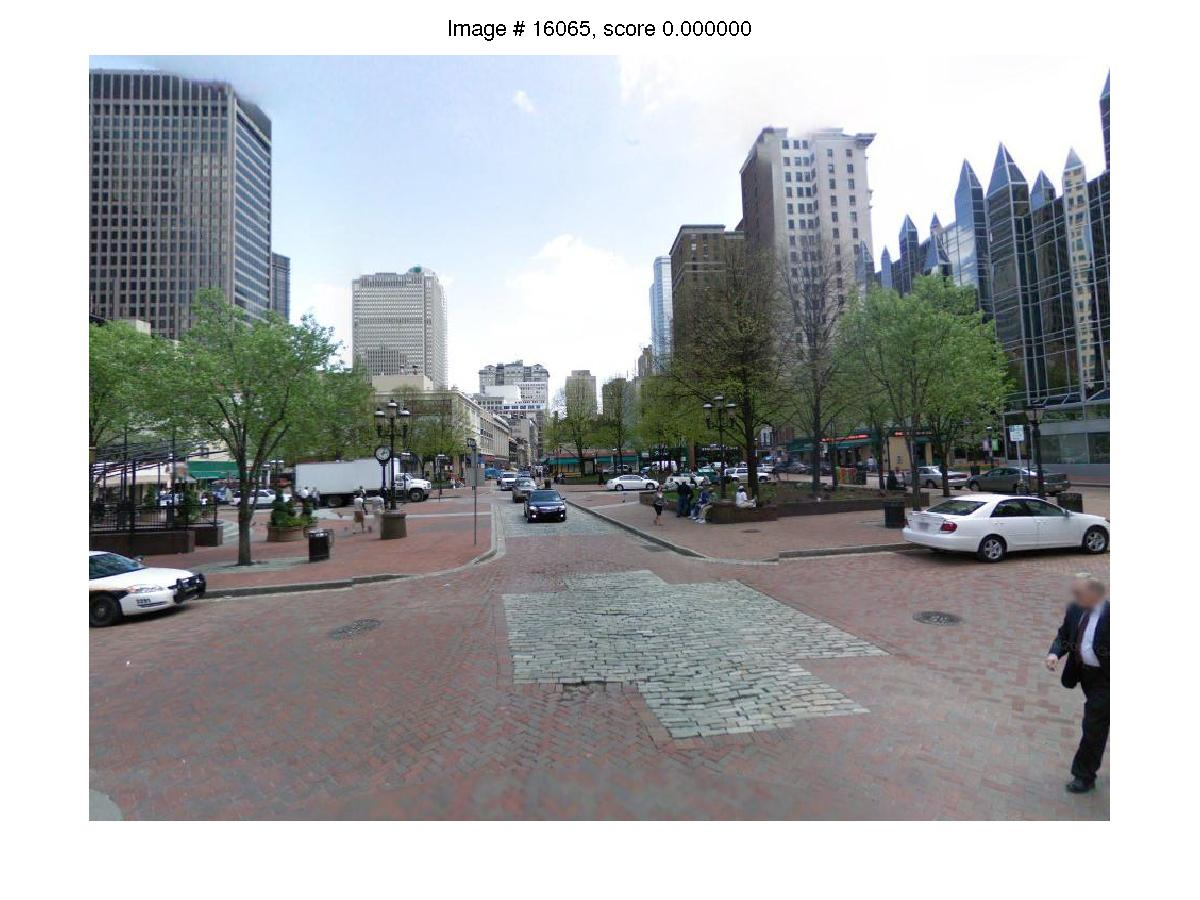
\includegraphics[trim = 35mm 30mm 35mm 30mm, clip=true, height=16mm]{imgs/Pval/exImproved03/improved02.jpg}}
        %         \colorbox{myRed}{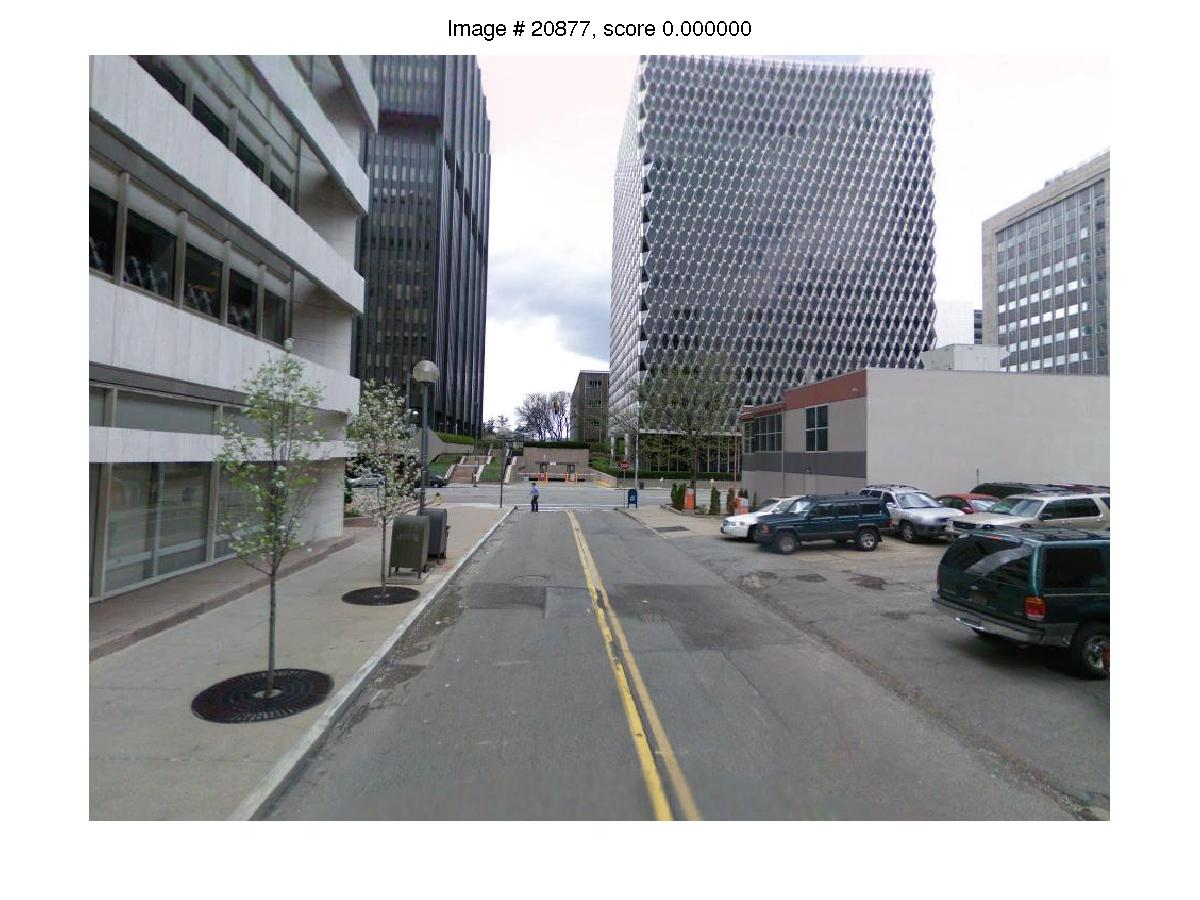
\includegraphics[trim = 35mm 30mm 35mm 30mm, clip=true, height=16mm]{imgs/Pval/exImproved03/improved03.jpg}}
        %         \colorbox{myRed}{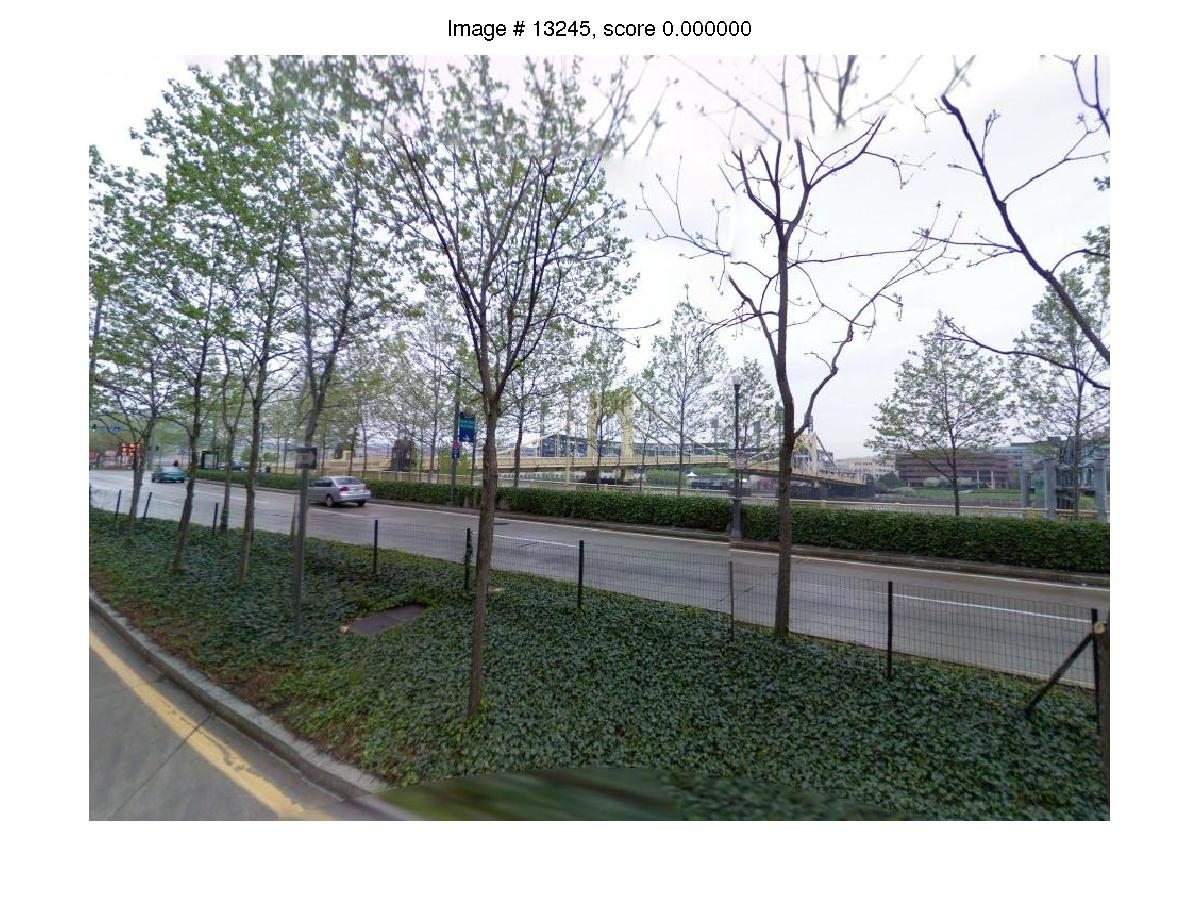
\includegraphics[trim = 35mm 30mm 35mm 30mm, clip=true, height=16mm]{imgs/Pval/exImproved03/improved04.jpg}}
        %     \end{minipage} 
        % \end{minipage}
        % \vspace{3mm}
        % \\
        %%%%%%%%%%% Example 3 %%%%%%%%%%%%%%%
        \begin{minipage}{0.34\linewidth}
            \centering
            \vspace{0mm}
            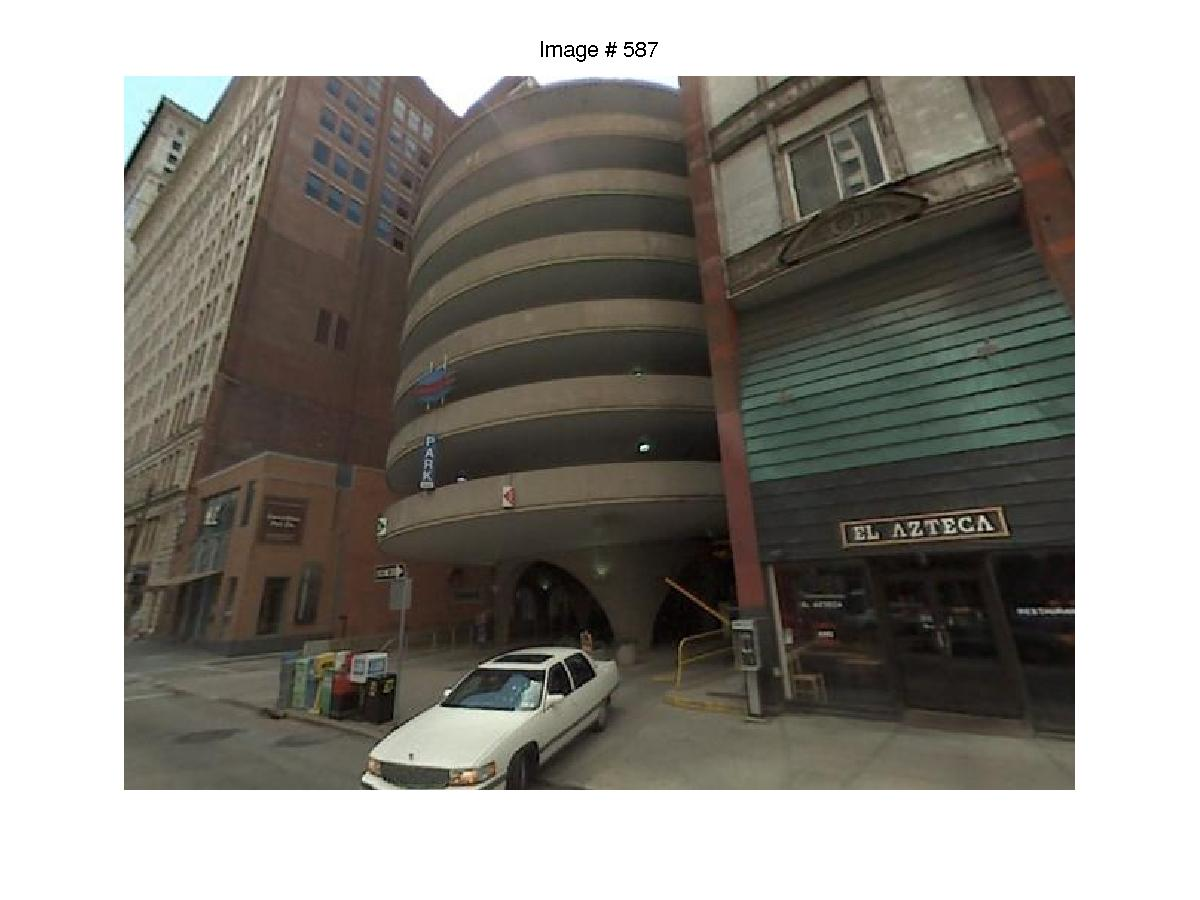
\includegraphics[trim = 45mm 40mm 45mm 30mm, clip=true, height=36mm]{imgs/Pval/exImproved04/query.jpg}
        \end{minipage}
        % Retrieved images
        \begin{minipage}{0.75\linewidth}
            % FV e-SVM
            \begin{minipage}{\linewidth} 
                \colorbox{myGreen}{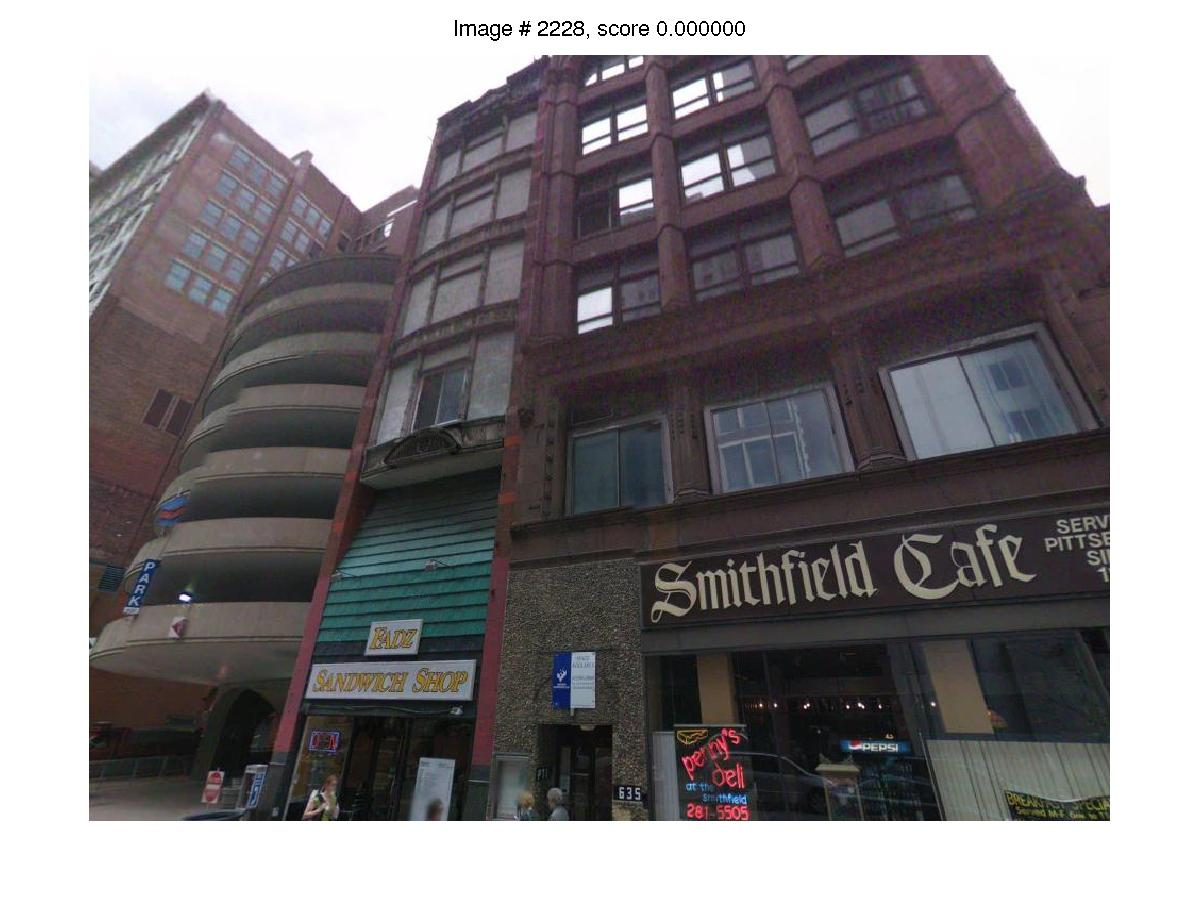
\includegraphics[trim = 35mm 30mm 35mm 30mm, clip=true, height=16mm]{imgs/Pval/exImproved04/improvedPval01.jpg}}
                \colorbox{myGreen}{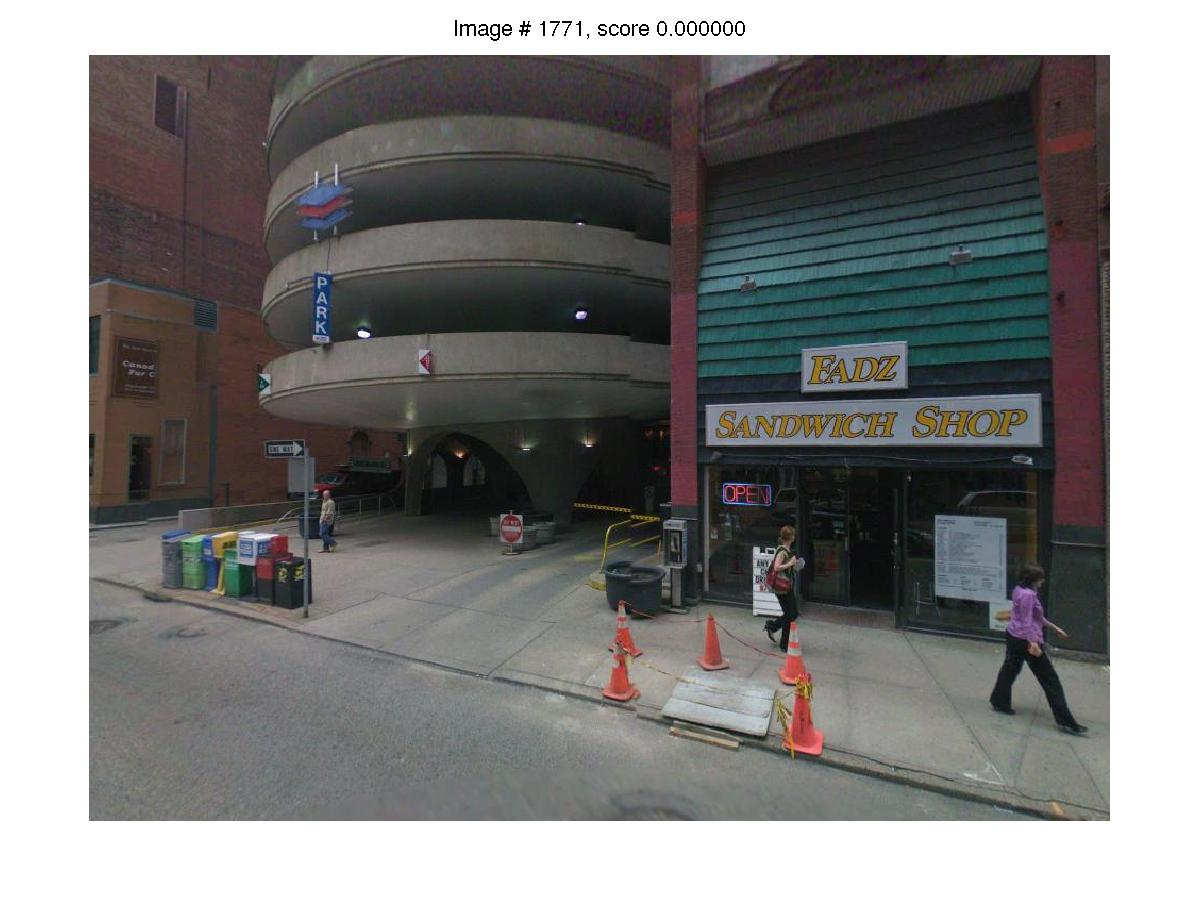
\includegraphics[trim = 35mm 30mm 35mm 30mm, clip=true, height=16mm]{imgs/Pval/exImproved04/improvedPval02.jpg}}
                \colorbox{myGreen}{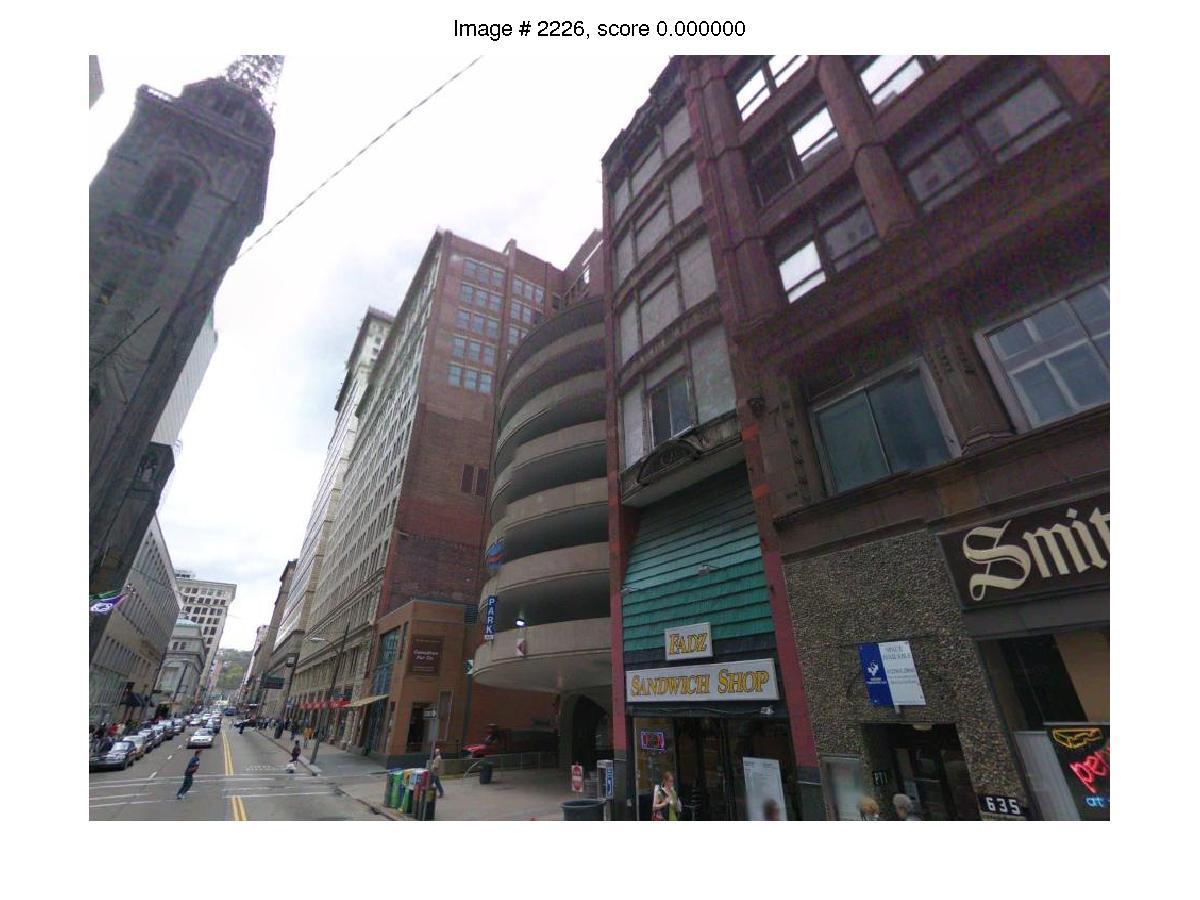
\includegraphics[trim = 35mm 30mm 35mm 30mm, clip=true, height=16mm]{imgs/Pval/exImproved04/improvedPval03.jpg}}
                \colorbox{myGreen}{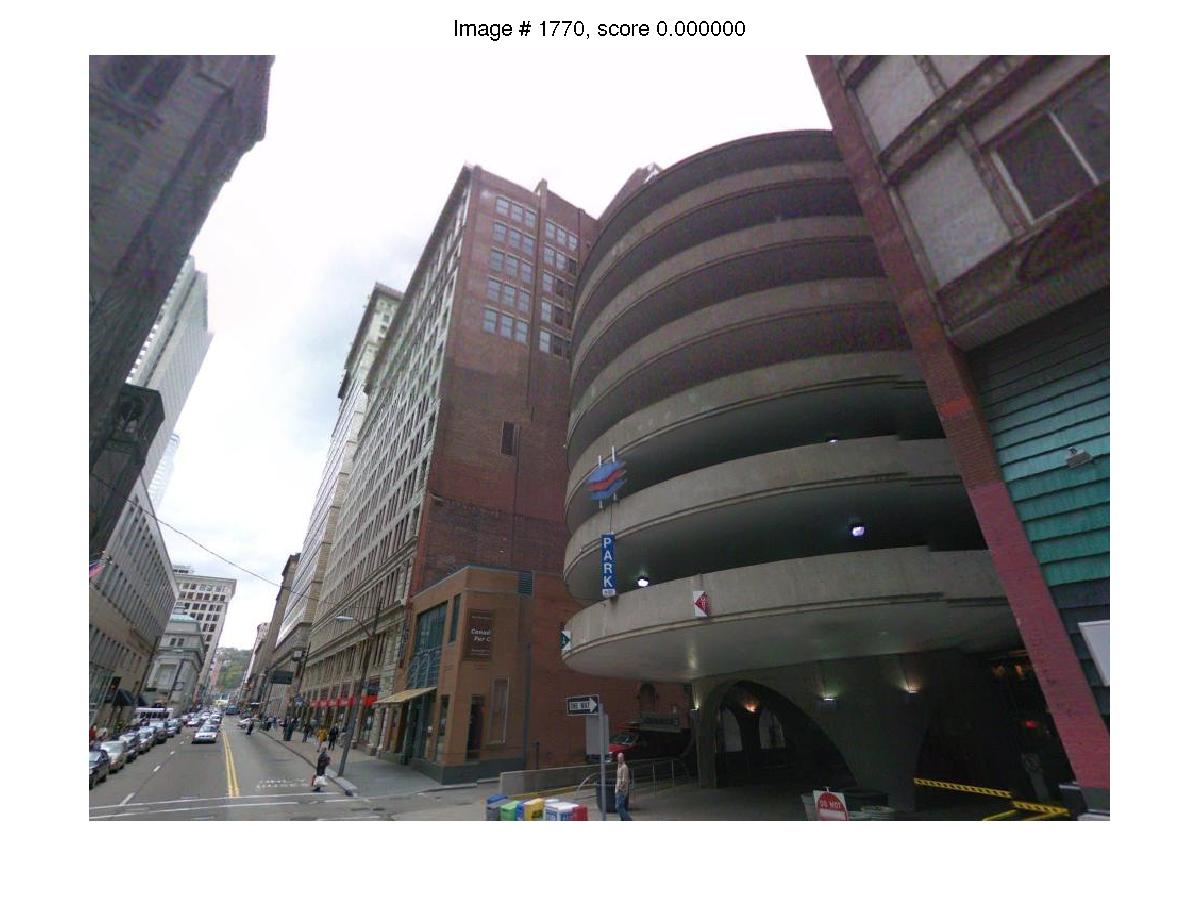
\includegraphics[trim = 35mm 30mm 35mm 30mm, clip=true, height=16mm]{imgs/Pval/exImproved04/improvedPval04.jpg}}
            \end{minipage}
            \\
            \begin{minipage}{\linewidth}
                \colorbox{myRed}{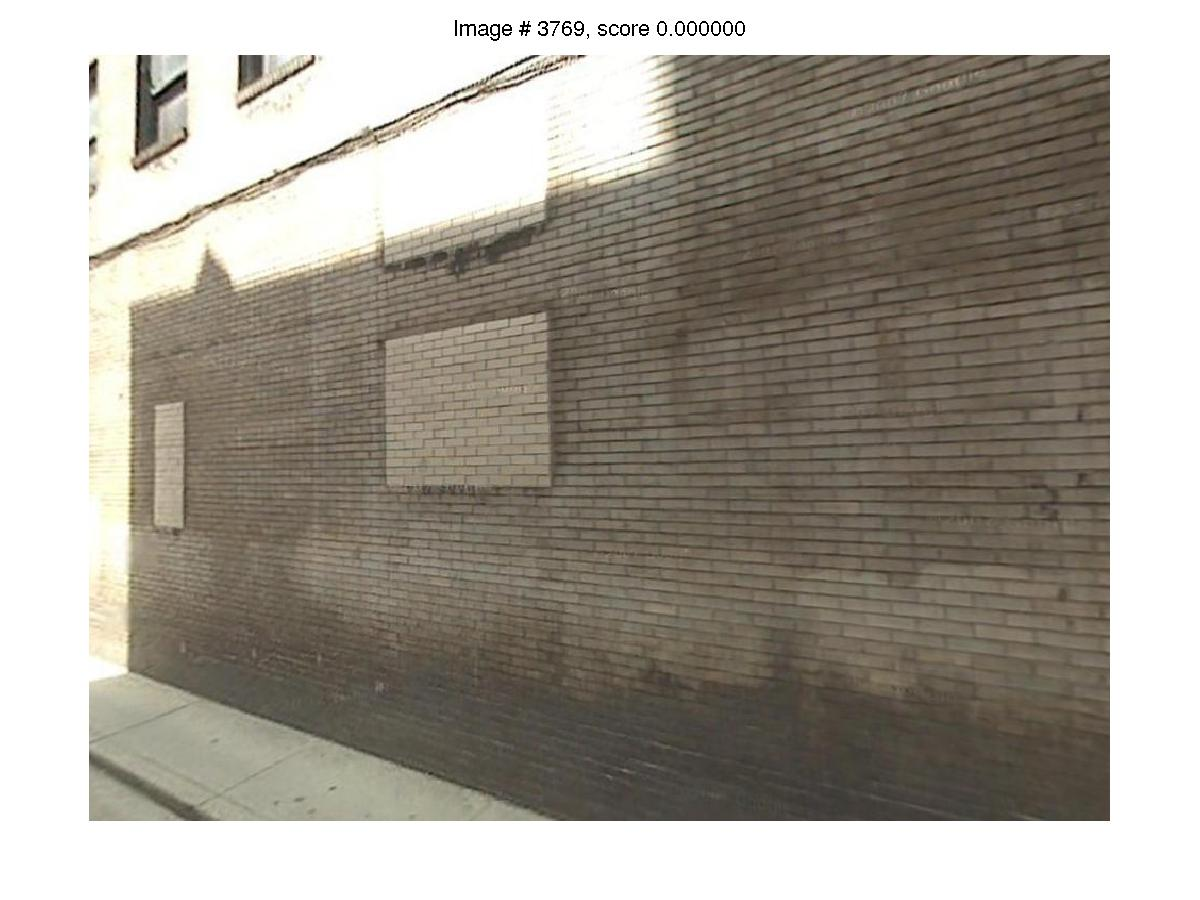
\includegraphics[trim = 35mm 30mm 35mm 30mm, clip=true, height=16mm]{imgs/Pval/exImproved04/improved01.jpg}}
                \colorbox{myRed}{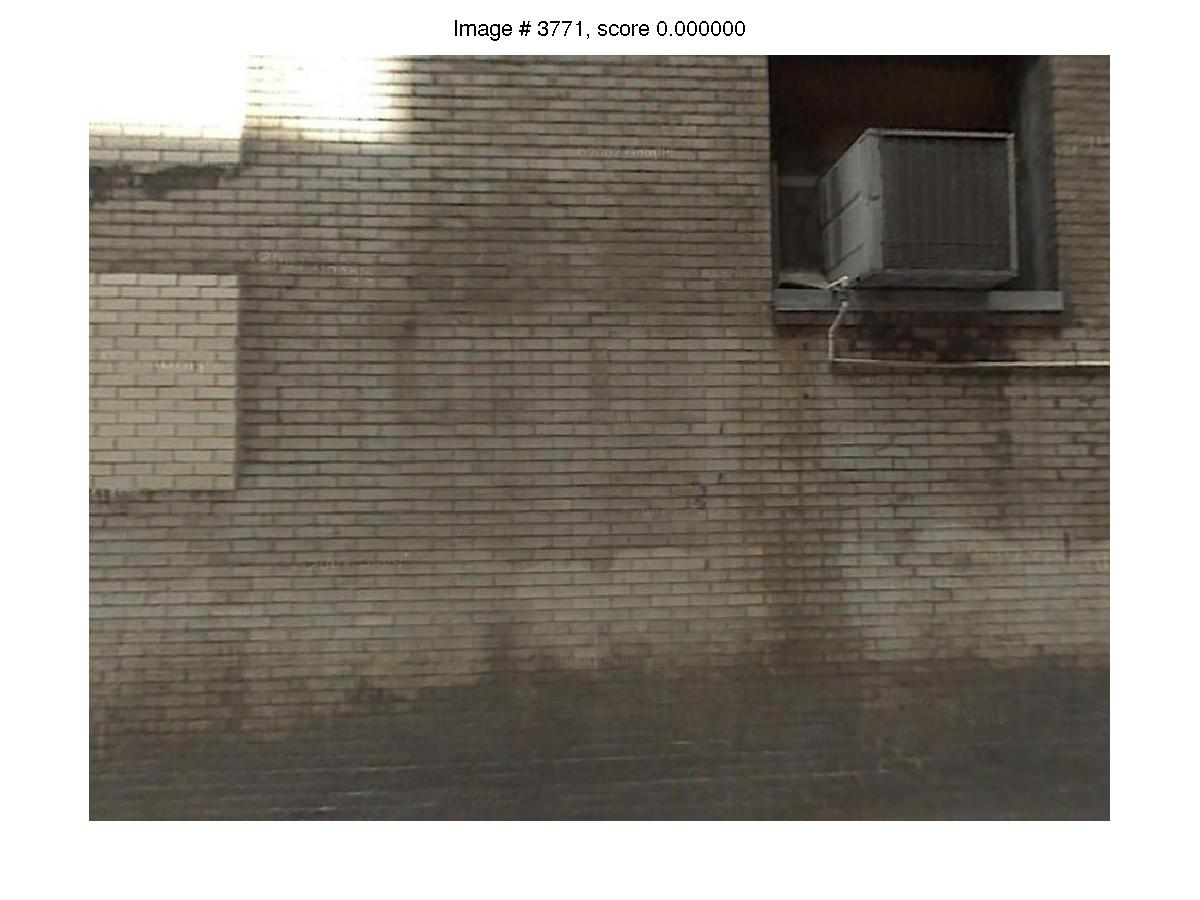
\includegraphics[trim = 35mm 30mm 35mm 30mm, clip=true, height=16mm]{imgs/Pval/exImproved04/improved02.jpg}}
                \colorbox{myRed}{\includegraphics[trim = 35mm 30mm 35mm 30mm, clip=true, height=16mm]{imgs/Pval/exImproved04/improved03.jpg}}
                \colorbox{myRed}{\includegraphics[trim = 35mm 30mm 35mm 30mm, clip=true, height=16mm]{imgs/Pval/exImproved04/improved04.jpg}}
            \end{minipage} 
        \end{minipage}
        \vspace{3mm}
        \\
        %%%%%%%%%%% MIX FAILURE CASES: good examples are Mix09 14 17 16 20
        %%%%%%%%%%% Example 4 %%%%%%%%%%%%%%%
        \begin{minipage}{0.34\linewidth}
            \centering
            \vspace{0mm}
            \includegraphics[trim = 45mm 40mm 45mm 30mm, clip=true, height=36mm]{imgs/Pval/exMix09/query.jpg}
        \end{minipage}
        % Retrieved images
        \begin{minipage}{0.75\linewidth}
            % FV e-SVM
            \begin{minipage}{\linewidth} 
                \colorbox{myGreen}{\includegraphics[trim = 35mm 30mm 35mm 30mm, clip=true, height=16mm]{imgs/Pval/exMix09/mixPval01.jpg}}
                \colorbox{myGreen}{\includegraphics[trim = 35mm 30mm 35mm 30mm, clip=true, height=16mm]{imgs/Pval/exMix09/mixPval02.jpg}}
                \colorbox{myRed}{\includegraphics[trim = 35mm 30mm 35mm 30mm, clip=true, height=16mm]{imgs/Pval/exMix09/mixPval03.jpg}}
                \colorbox{myGreen}{\includegraphics[trim = 35mm 30mm 35mm 30mm, clip=true, height=16mm]{imgs/Pval/exMix09/mixPval04.jpg}}
            \end{minipage}
            \\
            \begin{minipage}{\linewidth}
                \colorbox{myRed}{\includegraphics[trim = 35mm 30mm 35mm 30mm, clip=true, height=16mm]{imgs/Pval/exMix09/mix01.jpg}}
                \colorbox{myGreen}{\includegraphics[trim = 35mm 30mm 35mm 30mm, clip=true, height=16mm]{imgs/Pval/exMix09/mix02.jpg}}
                \colorbox{myRed}{\includegraphics[trim = 35mm 30mm 35mm 30mm, clip=true, height=16mm]{imgs/Pval/exMix09/mix03.jpg}}
                \colorbox{myRed}{\includegraphics[trim = 35mm 30mm 35mm 30mm, clip=true, height=16mm]{imgs/Pval/exMix09/mix04.jpg}}
            \end{minipage} 
        \end{minipage}
        \vspace{3mm}
        \\
        %%%%%%%%%%% Example 5 %%%%%%%%%%%%%%%
        \begin{minipage}{0.34\linewidth}
            \centering
            \vspace{0mm}
            \includegraphics[trim = 45mm 40mm 45mm 30mm, clip=true, height=36mm]{imgs/Pval/exMix19/query.jpg}
        \end{minipage}
        % Retrieved images
        \begin{minipage}{0.75\linewidth}
            % FV e-SVM
            \begin{minipage}{\linewidth} 
                \colorbox{myRed}{\includegraphics[trim = 35mm 30mm 35mm 30mm, clip=true, height=16mm]{imgs/Pval/exMix19/mixPval01.jpg}}
                \colorbox{myGreen}{\includegraphics[trim = 35mm 30mm 35mm 30mm, clip=true, height=16mm]{imgs/Pval/exMix19/mixPval02.jpg}}
                \colorbox{myGreen}{\includegraphics[trim = 35mm 30mm 35mm 30mm, clip=true, height=16mm]{imgs/Pval/exMix19/mixPval03.jpg}}
                \colorbox{myGreen}{\includegraphics[trim = 35mm 30mm 35mm 30mm, clip=true, height=16mm]{imgs/Pval/exMix19/mixPval04.jpg}}
            \end{minipage}
            \\
            \begin{minipage}{\linewidth}
                \colorbox{myRed}{\includegraphics[trim = 35mm 30mm 35mm 30mm, clip=true, height=16mm]{imgs/Pval/exMix19/mix01.jpg}}
                \colorbox{myRed}{\includegraphics[trim = 35mm 30mm 35mm 30mm, clip=true, height=16mm]{imgs/Pval/exMix19/mix02.jpg}}
                \colorbox{myGreen}{\includegraphics[trim = 35mm 30mm 35mm 30mm, clip=true, height=16mm]{imgs/Pval/exMix19/mix03.jpg}}
                \colorbox{myRed}{\includegraphics[trim = 35mm 30mm 35mm 30mm, clip=true, height=16mm]{imgs/Pval/exMix19/mix04.jpg}}
            \end{minipage} 
        \end{minipage}
        %%%%%%%%%%%%%%%%%%%%%%%%%%%%%%%%%%%%%

      \caption{
          \textbf{Examples  of correctly and incorrectly localized queries for the learnt bag-of-visual-words representation.}
          Each example shows a query image (left) together with correct (green) and incorrect (red) matches from the database obtained by learnt bag-of-visual-words representation \emph{p-val} method (top) and the standard bag-of-visual-words baseline (bottom). Note that the proposed method is able to recognize the place depicted in the query image despite changes in viewpoint, illumination and partial occlusion by other objects (trees, lamps) and buildings. Note also that bag-of-visual-words baseline is often confused by repeating patterns on facades and walls. 
      }
      \label{fig:images}
    \end{figure*}



   %%%%%%%%%%%%%%%%%
  \subsection{Fisher vectors}
  \label{sec:fisher_restuls}
  %%%%%%%%%%%%%%%%%
  
      %%% TABLE: Results 25k FV only
    \begin{table}[tbp]
      \begin{centering}
        \begin{table}[t!]
\begin{centering}
	\begin{tabularx}{0.89\linewidth}{|l|c c c c c|}
		\hline 
		\rowcolor{maroon!50}
		Method: & \multicolumn{5}{c|}{25k Pittsburgh} \\
		\hline 
		\hline 
		%%%%%%%%%%%%%%%%%%%%%%%%%%%%%%%%%%%%%%%%%%%%%%%%%%%%%%%%%%%%%%%%%%%%%%%%%%%%
		\rowcolor{maroon!50}
		recall@K [$\%$] & 1 & 2 & 5 & 10 & 20 \\
		\hline
		\rowcolor{maroon!10}
		BOW           & 28.7  & 35.7  & 45.8 & 53.7   & 61.5 \\
        \rowcolor{maroon!10}
		BOW p-val     & 33.0  & 40.3  & 50.2 & 58.7   &  66.4 \\
        \rowcolor{maroon!10}
		BOW w-norm  & 31.8  & 38.7  & 49.7 & 60.2   & 69.4 \\
        \hline
        %%%%%%%%%%%%%%%%%%%%%%%%%%%%%%%%%%%%%%%%%%%%%%%%%%%%%%%%%%%%%%%%%%%%%%%%%%%%
		\rowcolor{maroon!10}
		FV128         & 33.6  & 41.8  & 52.0 & 59.8   & 67.7  \\
		\rowcolor{maroon!10}
		FV128 p-val                 & \textbf{}       & \textbf{}     & \textbf{}     & \textbf{}     & \textbf{}  \\
    \rowcolor{maroon!10}
		\textbf{FV128 w-norm}     & \textbf{38.3}   & \textbf{47.5} & \textbf{57.7} & \textbf{65.8} & \textbf{72.7}  \\
    \hline  
    %%%%%%%%%%%%%%%%%%%%%%%%%%%%%%%%%%%%%%%%%%%%%%%%%%%%%%%%%%%%%%%%%%%%%%%%%%%%%
    \rowcolor{maroon!10}
    FV512         & 44.3 & 51.7   & 61.4  & 68.7   & 75.2  \\
    \rowcolor{maroon!10}
    \textbf{FV512 w-norm}   & \textbf{47.6}  & \textbf{55.4} & \textbf{65.1} & \textbf{72.4} & \textbf{78.8}  \\
    \hline
    %%%%%%%%%%%%%%%%%%%%%%%%%%%%%%%%%%%%%%%%%%%%%%%%%%%%%%%%%%%%%%%%%%%%%%%%%%%%%%
		\rowcolor{maroon!10}
		FV2048        & 46.9  & 54.1  & 63.8  & 70.5    & 76.8 \\
		\rowcolor{maroon!10}
		% FV2048 p-val  & \textbf{} & \textbf{} & \textbf{} & \textbf{} & \textbf{} &
  %       \textbf{} & \textbf{} & \textbf{} & \textbf{} & \textbf{}\\
        \rowcolor{maroon!10}
        \textbf{FV2048 w-norm}  & \textbf{50.2} & \textbf{57.3} & \textbf{67.0} & \textbf{73.8} & \textbf{78.0} \\
        \hline
        %%%%%%%%%%%%%%%%%%%%%%%%%%%%%%%%%%%%%%%%%%%%%%%%%%%%%%%%%%%%%%%%%%%%%%%%%%%%%%%%
  %       \rowcolor{maroon!10}
  %       FV8192        & 46.0  & 52.7 & 62.5 & 69.4 & 76.4 & - & - & - & - &  -   \\
  %       \rowcolor{maroon!10}
  %       \textbf{FV8192 w-norm}  & \textbf{48.4} & \textbf{55.6} & \textbf{65.4} & \textbf{72.6} & \textbf{79.0} & - & - & - & - & -\\
		% \hline
	\end{tabularx}
  \caption{ 
      % The percentage of correctly localized test queries for which the topK ranked database image is within $20$ meters   from the ground truth query position. The proposed method (svmFV) outperforms the baseline methods.
      \textbf{Results on Pittsburgh 25k dataset.} The fraction of correctly recognized queries (recall@K) vs. the number of top $K\in\{1,2,5,10,20\}$ retrieved database images for different Fisher vector dimensions $d\in\{128,512,2048\}$ and BOW for different calibration methods. The learnt Fisher vector descriptors by the  \emph{w-norm} method consistently improve over the raw Fisher vector descriptors across the whole range of $K$ and all dimensions.    
  }

\label{tab:recall01}
\end{centering}
\end{table}

        \caption{ 
          \textbf{Evaluation of the learnt Fisher vector representation on the Pittsburgh 25k \cite{Gronat13} dataset.}
           The table shows the fraction of correctly recognized queries (recall@K) for the different values of $K\in\{1,2,5,10,20\}$ retrieved database images. 
	   The learnt Fisher vector representation (FV \emph{w-norm}) consistently improves over the standard Fisher vector matching baseline (FV) for all dimensions $d\in\{128,512,2048\}$.
        }
        \label{tab:recallFV}
      \end{centering}
    \end{table}

    %%% PLOT: FV recall curves
    \begin{figure}[tbp]
        \centering
        \includegraphics[width=1\linewidth]{imgs/plotPitt25kNoBOW}  
        %\includegraphics[trim=35mm 70mm 40mm 75mm, clip=true, width=\linewidth]{imgs/plotPitt25k}    
        \vspace*{-7mm}
        \caption{
            \textbf{Evaluation of the learnt Fisher vector representation on the Pittsburgh 25k \cite{Gronat13} dataset.} 
            The graph shows the fraction of correctly recognized queries (recall@K, y-axis) vs. the number of top $K$ retrieved database images for the raw Fisher vector baseline (FV) for different dimensions compared to the learnt representation (\emph{w-norm}). Note the consistent improvements over all lengths of shortlist $K$ for all dimensions.
        }
        \label{fig:recall}
    \end{figure}

    Results of the proposed per-location learning method for the Fisher vector image representation for different dimensions $d\in\{128, 512, 2048\}$ 
    are shown in table~\ref{tab:recallFV} and figure~\ref{fig:recall}.
    Similar to bag-of-visual-words, the learnt representation (w-norm) significantly improves the place recognition performance over the baseline Fisher vector (FV) matching without learning. The improvements are consistent across different lengths of shortlist $K$ and for different dimensionality of the Fisher vector representation. 
    We report results only for the w-norm calibration as we found that the p-val calibration did not perform for the learnt Fisher vector classifiers (top 1 recall of 25.3\% compared to baseline performance of 33.6\% for dimension 128). When examining the results, we believe this may be attributed to the fact that Fisher vectors are low dimensional compared to the extremely high-dimensional (d=100,000) bag-of-visual-words representation, which affects the distribution of the classifier scores on the negative test data. 
    Examples of correctly and incorrectly localized queries are shown in figure~\ref{fig:images}. 
%    The query image is show in the left column and the shortlist of the top four retrieved images is shown on the right. For each query, the first row shows images retrieved by the learnt Fisher vector descriptor for dimension $d=128$, while the second row shows images retrieved by raw Fisher vector of the same dimension.
    
        Finally, we test the learnt Fisher vector representation on the larger Pittsburgh 55k dataset. As shown in table~\ref{tab:recallFV55k} the proposed per-location learning method still consistently improves the performance over the raw Fisher vector descriptors across the different descriptor dimensions and lengths of the shortlist. 

\noindent
        Next, we compare the performance of the two learnt representations relative to their memory footprints.  

    %%% FIGURE: Visualization for FV  
    \begin{figure*}[tbp]
      %%%%%%%%%%% Example 1 %%%%%%%%%%%%%%%
\begin{minipage}{1.0\linewidth}
\end{minipage}
% QUERY image
\begin{minipage}{0.34\linewidth}
    \centering
    \vspace{5mm}
    \includegraphics[height=40mm]{imgs/ex1/query.jpg}
\end{minipage}
% Retrieved images
\begin{minipage}{0.75\linewidth}
    % FV e-SVM
    \begin{minipage}{\linewidth} 
        \colorbox{myGreen}{\includegraphics[height=16mm]{imgs/ex1/FVsvm1.jpg}}
        \colorbox{myGreen}{\includegraphics[height=16mm]{imgs/ex1/FVsvm2.jpg}}
        \colorbox{myGreen}{\includegraphics[height=16mm]{imgs/ex1/FVsvm3.jpg}}
        \colorbox{myGreen}{\includegraphics[height=16mm]{imgs/ex1/FVsvm4.jpg}}
    \end{minipage}
    \\
    \begin{minipage}{\linewidth}
        \colorbox{myRed}{\includegraphics[height=16mm]{imgs/ex1/FV1.jpg}}
        \colorbox{myRed}{\includegraphics[height=16mm]{imgs/ex1/FV2.jpg}}
        \colorbox{myRed}{\includegraphics[height=16mm]{imgs/ex1/FV3.jpg}}
        \colorbox{myRed}{\includegraphics[height=16mm]{imgs/ex1/FV4.jpg}}
    \end{minipage} 
\end{minipage}
\\
%%%%%%%%%%% Example 2 %%%%%%%%%%%%%%%
\begin{minipage}{0.34\linewidth}
    \centering
    \vspace{0mm}
    \includegraphics[height=36mm]{imgs/ex2/query.jpg}
\end{minipage}
% Retrieved images
\begin{minipage}{0.75\linewidth}
    % FV e-SVM
    \begin{minipage}{\linewidth} 
        \colorbox{myGreen}{\includegraphics[height=16mm]{imgs/ex2/FVsvm1.jpg}}
        \colorbox{myGreen}{\includegraphics[height=16mm]{imgs/ex2/FVsvm2.jpg}}
        \colorbox{myGreen}{\includegraphics[height=16mm]{imgs/ex2/FVsvm3.jpg}}
        \colorbox{myGreen}{\includegraphics[height=16mm]{imgs/ex2/FVsvm4.jpg}}
    \end{minipage}
    \\
    \begin{minipage}{\linewidth}
        \colorbox{myRed}{\includegraphics[height=16mm]{imgs/ex2/FV1.jpg}}
        \colorbox{myRed}{\includegraphics[height=16mm]{imgs/ex2/FV2.jpg}}
        \colorbox{myRed}{\includegraphics[height=16mm]{imgs/ex2/FV3.jpg}}
        \colorbox{myRed}{\includegraphics[height=16mm]{imgs/ex2/FV4.jpg}}
    \end{minipage} 
\end{minipage}
\vspace{3mm}
\\
%%%%%%%%%%% Example 3 %%%%%%%%%%%%%%%
\begin{minipage}{0.34\linewidth}
    \centering
    \vspace{0mm}
    \includegraphics[height=36mm]{imgs/ex3/query.jpg}
\end{minipage}
% Retrieved images
\begin{minipage}{0.75\linewidth}
    % FV e-SVM
    \begin{minipage}{\linewidth} 
        \colorbox{myGreen}{\includegraphics[height=16mm]{imgs/ex3/FVsvm1.jpg}}
        \colorbox{myRed}{\includegraphics[height=16mm]{imgs/ex3/FVsvm2.jpg}}
        \colorbox{myGreen}{\includegraphics[height=16mm]{imgs/ex3/FVsvm5.jpg}}
        \colorbox{myGreen}{\includegraphics[height=16mm]{imgs/ex3/FVsvm4.jpg}}
    \end{minipage}
    \\
    \begin{minipage}{\linewidth}
        \colorbox{myRed}{\includegraphics[height=16mm]{imgs/ex3/FV1.jpg}}
        \colorbox{myGreen}{\includegraphics[height=16mm]{imgs/ex3/FV2.jpg}}
        \colorbox{myRed}{\includegraphics[height=16mm]{imgs/ex3/FV3.jpg}}
        \colorbox{myRed}{\includegraphics[height=16mm]{imgs/ex3/FV4.jpg}}
    \end{minipage} 
\end{minipage}
\vspace{3mm}
\\
%%%%%%%%%%% Example 4 %%%%%%%%%%%%%%%
\begin{minipage}{0.34\linewidth}
    \centering
    \vspace{0mm}
    \includegraphics[height=36mm]{imgs/ex4/query.jpg}
\end{minipage}
% Retrieved images
\begin{minipage}{0.75\linewidth}
    % FV e-SVM
    \begin{minipage}{\linewidth} 
        \colorbox{myGreen}{\includegraphics[height=16mm]{imgs/ex4/FVsvm1.jpg}}
        \colorbox{myRed}{\includegraphics[height=16mm]{imgs/ex4/FVsvm2.jpg}}
        \colorbox{myGreen}{\includegraphics[height=16mm]{imgs/ex4/FVsvm5.jpg}}
        \colorbox{myGreen}{\includegraphics[height=16mm]{imgs/ex4/FVsvm4.jpg}}
    \end{minipage}
    \\
    \begin{minipage}{\linewidth}
        \colorbox{myRed}{\includegraphics[height=16mm]{imgs/ex4/FV1.jpg}}
        \colorbox{myGreen}{\includegraphics[height=16mm]{imgs/ex4/FV2.jpg}}
        \colorbox{myRed}{\includegraphics[height=16mm]{imgs/ex4/FV3.jpg}}
        \colorbox{myRed}{\includegraphics[height=16mm]{imgs/ex4/FV4.jpg}}
    \end{minipage} 
\end{minipage}
%%%%%%%%%%%%%%%%%%%%%%%%%%%%%%%%%%%%%

            \caption{
          \textbf{Examples of correctly and incorrectly localized queries for the learnt Fisher vector representation.}
          Each example shows a query image (left) together with correct (green) and incorrect (red) matches from the database obtained by the learnt Fisher vector representation \emph{w-norm} method (top) and the standard Fisher vector baseline (bottom) for dimension 128. Note that the proposed method is able to recognize the place depicted in the query image despite changes in viewpoint, illumination and partial occlusion by other objects (trees, lamps) and buildings. 
          Note that the baseline methods often finds images depicting the same buildings but in a distance whereas our learnt representation often finds a closer view better matching the content of the query.  
%          Note also that bag-of-visual-words baseline is often confused by repeating patterns on facades and walls. 
%        \textbf{Examples of improvements and failure cases for \emph{w-norm} method on Fisher vectors.}
%        Each example shows a query image (left) together with correct (green) and incorrect (red) matches from the database obtained by \emph{w-norm} method (top) and the raw Fisher vector descriptor baseline (bottom). For each method we show the top 4 matches from the database using 128-dimensional descriptors.        
%      
}
      \label{fig:images_bow}
    \end{figure*}
    
    %%% TABLE: results on Pittsburgh 55k
    \begin{table}[bh]
      \begin{centering}
        \begin{table}[t!]
\begin{centering}
	\begin{tabularx}{0.89\linewidth}{|l|c c c c c|}
		\hline 
		\rowcolor{maroon!50}
		Method: & \multicolumn{5}{c|}{55k Pittsburgh} \\
		\hline 
		\hline 
		%%%%%%%%%%%%%%%%%%%%%%%%%%%%%%%%%%%%%%%%%%%%%%%%%%%%%%%%%%%%%%%%%%%%%%%%%%%%
		\rowcolor{maroon!50}
		recall@K [$\%$] & 1 & 2 & 5 & 10 & 20\\
		\hline
		\rowcolor{maroon!10}
		BOW       & 8.7 & 11.0 & 17.3 & 22.8 & 25.4  \\
    \hline
    %%%%%%%%%%%%%%%%%%%%%%%%%%%%%%%%%%%%%%%%%%%%%%%%%%%%%%%%%%%%%%%%%%%%%%%%%%%%
		\rowcolor{maroon!10}
		FV128     & 10.9 & 14.1 & 20.2 & 26.4 & 33.2 \\
		\rowcolor{maroon!10}
		\textbf{FV128 w renorm}  & \textbf{13.5}  &  \textbf{17.7}  &  \textbf{25.0}  &  \textbf{31.8}  &  \textbf{39.0} \\
    \hline  
    %%%%%%%%%%%%%%%%%%%%%%%%%%%%%%%%%%%%%%%%%%%%%%%%%%%%%%%%%%%%%%%%%%%%%%%%%%%%%
    \rowcolor{maroon!10}
    FV512   & 17.3 &  21.1 &  28.4 &  34.2 &  40.3 \\      
    \rowcolor{maroon!10}
    % FV512 p-val   & \textbf{}  & \textbf{} & \textbf{} & \textbf{} & \textbf{}  &
    %                          \textbf{} &  \textbf{} &  \textbf{}  & \textbf{} &  \textbf{} \\
    \rowcolor{maroon!10}
    \textbf{FV512 w renorm}  & \textbf{19.8} &  \textbf{25.1} &  \textbf{32.7}  & \textbf{38.7} &  \textbf{46.0} \\
    \hline
    %%%%%%%%%%%%%%%%%%%%%%%%%%%%%%%%%%%%%%%%%%%%%%%%%%%%%%%%%%%%%%%%%%%%%%%%%%%%%%
		\rowcolor{maroon!10}
		FV2048        & 19.2 & 23.5 & 29.9 &  35.2 &  41.9 \\
		\rowcolor{maroon!10}
		% FV2048 p-val  & \textbf{} & \textbf{} & \textbf{} & \textbf{} & \textbf{} &
  %       \textbf{} & \textbf{} & \textbf{} & \textbf{} & \textbf{}\\
        \rowcolor{maroon!10}
        \textbf{FV2048 w renorm}  & \textbf{20.8} & \textbf{25.9} & \textbf{33.1} & \textbf{38.7} & \textbf{45.9} \\
        \hline
        %%%%%%%%%%%%%%%%%%%%%%%%%%%%%%%%%%%%%%%%%%%%%%%%%%%%%%%%%%%%%%%%%%%%%%%%%%%%%%%%
  %       \rowcolor{maroon!10}
  %       FV8192        & 46.0  & 52.7 & 62.5 & 69.4 & 76.4 & - & - & - & - &  -   \\
  %       \rowcolor{maroon!10}
  %       \textbf{FV8192 w renorm}  & \textbf{48.4} & \textbf{55.6} & \textbf{65.4} & \textbf{72.6} & \textbf{79.0} & - & - & - & - & -\\
		% \hline
	\end{tabularx}
	\caption{ \textcolor{myRed}{}
%		The percentage of correctly localized test queries for which the topK ranked database image is within $20$ meters from the ground truth query position. The proposed method (svmFV) outperforms the baseline methods.
The fraction of correctly recognized queries (recall@K) vs. the number of top $K\in\{1,2,5,10,20\}$ retrieved database images for different Fisher vector dimensions $d\in\{128,512,2048\}$. The learnt descriptors by the proposed method (FV w renorm) consistently improve over the raw Fisher vector descriptors across the whole range of $K$ and all dimensions on 55k Pittsburgh image datasets.		
}
\label{tab:recall02}
\end{centering}
\end{table}

                \caption{ 
          \textbf{Evaluation of the learnt Fisher vector representation on the Pittsburgh 55k dataset.}
           The table shows the fraction of correctly recognized queries (recall@K) for the different values of $K\in\{1,2,5,10,20\}$ retrieved database images. 
	   The learnt Fisher vector representation (FV w-norm) consistently improves over the standard Fisher vector matching baseline (FV) for all dimensions $d\in\{128,512,2048\}$.
        }
        \label{tab:recallFV55k}
      \end{centering}
    \end{table}

 
  %%%%%%%%%%%%%%%%
%    \subsection{Memory complexity analysis}
  \subsection{Analysis of recognition accuracy vs. compactness}
  \label{sec:memory_results}
  %%%%%%%%%%%%%%%%
  Here we analyze the recognition accuracy of the learnt representations vs. their compactness measured by their memory footprint on the Pittsburgh 25k image dataset.
  Ideally, we wish to learn a more compact representation, that still improves the recognition accuracy. However, usually there is a trade-off between the discriminative power of the representation and its size, where having a more compact representation reduces the recognition accuracy~\cite{Jegou12}. We observe a similar behavior but our learnt representation results in a higher recognition accuracy for a given size, or alternatively, significantly reduces the size of the representation for a given accuracy.   
   The results are summarized in figure~\ref{fig:memory}.
%    Figure~\ref{fig:memory} compares the performance of the proposed per-location learning method for the two different image representations  compared to their memory requirements. 
     The figure shows the recognition performance (y-axis) for the different dimensionality of the Fisher vector representation, which corresponds to different memory footprints (x-axis). For example, for $d=128$ the memory footprint is about 24~MB, whereas for $d=2048$ the memory footprint is about 384~MB. Note that the x-axis is in log-scale. The bag-of-visual-words representation has a fixed dimensionality (and fixed memory footprint) and hence each bag-of-visual-words method is shown only as a single point on the graph.  For Fisher vectors, the results demonstrate that for a given level of accuracy (y-axis) the proposed method learns a more compact (lower-dimensional) representation (x-axis). For example, our learnt 128-dimensional descriptor (memory footprint of 24 MB) achieves a similar accuracy (around 65\%) as the 256-dimensional raw Fisher descriptor (memory footprint of 51MB). This corresponds to 50\% memory savings for the same level of recognition performance. Note that similar to~\cite{Jegou12}, we observe decrease in performance at high-dimensions for both the FV baseline and our method. The results also demonstrate the benefits of using the compact FV descriptors compared to the bag-of-visual-words baseline achieving significantly better recognition accuracy for a similar memory footprint.
    
    %%% FIGURE: Memory efficiency
    \begin{figure}[t!]
        \centering
        \includegraphics[width=1.1\linewidth]{imgs/FVmemory02}    
        \caption{
            \textbf{The recognition performance vs. the memory requirements for the Pittsburgh 25k dataset.} 
            The fraction of correctly localized queries at the top 10 retrieved images (y-axis) vs. the memory footprint (x-axis) for the different representations. For Fisher vectors, the learnt descriptor (FV \emph{w-renorm}) clearly outperforms the raw Fisher vector descriptor (FV) for all dimensions corresponding to different memory footprints (x-axis). 
            Learnt per-location representations for the bag-of-visual-words model (BOW p-val and BOW w-norm) also improve performance over the raw bag-of-visual-words (BOW). However, the Fisher vectors provide much better recognition performance for the same memory footprint.  
        }
        \label{fig:memory}
    \end{figure}


%%%%%%%%%%%%%%%%%%%%%
\section{Conclusions}
%%%%%%%%%%%%%%%%%%%%%
We have shown that place recognition can be cast as a classification problem and have used geotags as a readily-available supervision to
train an ensemble of classifiers, one for each location in the database. As only few positive examples are available for each
location, we have developed two procedures to calibrate the output of each classifier without the need for additional positive training
data. We have shown that learning per-location representations improves the place recognition performance over the raw bag-of-visual-words and
Fisher vector matching baselines. The developed calibration methods are not specific to place recognition and can be useful for other
per-exemplar classification tasks, where only a small number of positive examples are available~\cite{Malisiewicz11}.



\begin{acknowledgements}
   This work was supported by the MSR-INRIA laboratory, the EIT-ICT labs, Google and the ERC project LEAP.
   {
   %\small
   \noindent
   Supported by the Intelligence Advanced Research Projects Activity (IARPA) via Air Force Research Laboratory. The U.S. Government is authorized to reproduce and distribute reprints for governmental purposes notwithstanding any copyright annotation thereon. Disclaimer:  The views and conclusions contained herein are those of the authors and should not be interpreted as necessarily representing the official policies or endorsements, either expressed or implied, of IARPA, AFRL or the U.S. Government.
   }
\end{acknowledgements}



\bibliographystyle{spmpsci}      % mathematics and physical sciences

{\footnotesize
\bibliography{shortstrings,vggroup,cvww_template,mybib}
}

\end{document}
% end of file template.tex

